%--------------------------------------------------------------------------------------------------
% ips-phd-thesis-eng-apa.tex v1.3 (see the end of the file for modification
% history)
% To be used with ipsthesis.cls v1.3
% 
% A template for creating a PhD thesis in English using the APA 6th edition
% reference formatting
% with several accompanying files.  
% By Tea Tušar <tea.tusar@ijs.si>
%
% IMPORTANT NOTE: Biber must be used as the backhand for processing
% bibliographies, not bibtex!
%
% To compile this template, you need to run the following sequence of commands:
% 1. pdflatex  ips-phd-thesis-eng-apa
% 2. biber     ips-phd-thesis-eng-apa
% 3. makeindex ips-phd-thesis-eng-apa (optional, if you want an index)
% 4. pdflatex  ips-phd-thesis-eng-apa 
% 5. pdflatex  ips-phd-thesis-eng-apa
%-------------------------------------------------------------------------------

\documentclass[phd,eng,apa]{ipsthesis}
%
%-------------------------------------------------------------------------------
%  
% PREAMBULE
%-------------------------------------------------------------------------------
%
% Files with bibliographies 
\addbibresource{Moje-2017 - PhD citations.bib}
%\bibilography{Moje-2017 - PhD citations.bib}
%
% Define here all other packages and commands you need for your thesis, for 
% example:
\usepackage{color}
\usepackage{soul} %\hl command
\usepackage{longtable}
\usepackage{todonotes}
\usepackage{tikz} %\checkmark
\usepackage{listings} % for XML formatting
\usepackage{float} % for suppressing floating of tables/images
\usepackage{adjustbox} % For resizing tables
%For landscape related work table
\usepackage{pdflscape}
\usepackage{amsmath} % For nicer multi-line math
\usepackage{multirow} % For combining rows in the table
\usepackage{makecell} % For multi-row cells in the table

\DeclareLanguageMapping{american}{american-apa}
\DeclareLanguageMapping{slovene}{slovenian-apa}
%-------------------------------------------------------------------------------
%  
% DOCUMENT
%-------------------------------------------------------------------------------
\begin{document}
%-------------------------------------------------------------------------------
%
% FRONT MATTER
%-------------------------------------------------------------------------------
%
\frontmatter
%
\selectlanguage{american}
\pagestyle{fancy}

% Title pages
%--------------------------------------------------------------------------------------------------
% 
% INPUT FOR THE TITLE PAGES
%--------------------------------------------------------------------------------------------------
% 
% Author
\author{Luka Bradesko}         
%
% Title in English (use \protect\\ instead of \\ to create a line break)
\titleEnglish{Knowledge Acquisition through Natural Language Conversation and Crowdsourcing}
%
% Title in Slovene (use \protect\\ instead of \\ to create a line break)
\titleSlovene{Pridobivanje Strukturiranega Znanja skozi Pogovor ter s Pomocjo Mnozicenjai}
%
% Supervisor (title and name, affiliation)
\supervisorOne{Doc.\ Dunja Mladenic}{Jozef Stefan Institute, Ljubljana, Slovenia}
%
% Co-supervisor (title and name, affiliation), optional
%\supervisorTwo{Prof.\ Name Surname2}{Institution2, Place, Country}
%
% Co-supervisor (title and name, affiliation), optional
%\supervisorThree{Prof.\ Name Surname3}{Institution3, Place, Country}
%
% Evaluation board chairman (title and name, affiliation)
\evaluationBoardChairman{Dr.\ Michael Witbrock}{IBM, New York, New York}
%
% Evaluation board member #1 (title and name, affiliation)
\evaluationBoardMemberOne{Prof.\ Erjavec}{Jozef Stefan Institute, Ljubljana, Slovenia}
%
% Evaluation board member #2 (title and name, affiliation)
\evaluationBoardMemberTwo{Prof.\ Savnik}{Univerza v Novi Gorici, Nova Gorica, Slovenia}
% 
% Date
\thesismonth{April}
\thesisyear{2017}
%
\maketitle 

% Dedication (optional)
%--------------------------------------------------------------------------------------------------
% 
% INPUT FOR THE DEDICATION
%--------------------------------------------------------------------------------------------------
\dedication{To Vanessa}
\makededication


% Acknowledgments
%-------------------------------------------------------------------------------
% 
\chapter*{Acknowledgments}
\pdfbookmark[0]{Acknowledgments}{Acknowledgments}
%-------------------------------------------------------------------------------
I would like to express great appreciation to my PhD supervisor Prof. Dunja 
Mladenić for her support, guidance and advice throughout my studies. 
I would like to thank my co-autors, collaborators and
my colleagues from Jožef Stefan Institute for many valuable discussions, 
insights and suggestions. 
I would also like to thank the members of my doctoral committe, 
Michael Witbrock, Tomaž Erjavec and Iztok Savnik for their valuable comments and
remarks. 
Special thanks thanks go to Michael Witbrock, Janez Starc and Dane Sulič for
multiple years of help with the design and development of Curious Cat 
implementation. I thank to all of our 728 users who contributed 
to the experiment of the KA system, and Dr. Dave Schneider in particular and 
Cycorp management and members of the Cycorp technical staff (including Chris 
Deaton and Dr. David Baxter) more generally for licensing, for their kind 
assistance with APIs, KR advice and other assistance as we constructed and 
tested Curious Cat.
Additionally I would like to thank Marko Grobelnik and colleagues from
Artificial Intelligence Laboratory (Jožef Stefan Institute) for providing a 
good work and research environment, enabling me to focus on the research and
implementation required to finish this thesis. Similar thanks goes to AI team
at Bloomberg L.P., for encouraging me and allowing me to abstain from my work
duties while focusing on the thesis.

Finally I wish to thank Vanessa, my parents Agata and Bernard and my brothers
Marko and Valter for their support and encouragement.

\rule{0.5\textwidth}{.4pt}

This work was supported and partially financed by European Commission under
LARKC (The Large Knowledge Collider: a platform for large scale integrated
reasoning and Web-search, FP7-215535), MOBIS (Personalized Mobility Services 
for energy efficiency and security through advanced Artificial Intelligence 
techniques, FP7-318452), ENVISION (EmpoweriNg European SME business model 
Innovation ,ICT-2009-249120), OPTIMUM (Multi-source Big Data Fusion Driven 
Proactivity for Intelligent Mobility, H2020-MG-636160) and personally by 
Dr. Michael Witbrock.

 
% English abstract
%-------------------------------------------------------------------------------
% 
\chapter*{Abstract}
\pdfbookmark[0]{Abstract}{Abstract}
%-------------------------------------------------------------------------------

Knowledge Acquisition is an important part of Artificial Intelligence. Having high-quality structured knowledge helps to advance other research activities that depend on a rich understanding of the world around us. Due to a lack of reliable automation strategies this problem has been mostly attacked through hand-annotation and structuring by human experts. In recent years, there have been attempts to scale the manual approach through crowd-sourcing.

Although numerous systems and methods for crowd-sourced knowledge acquisition have been developed to solve the problem of manpower, the issues of high cost, task specification, targeting, consistency, and eventual quality of acquired knowledge, seem to persist.

The thesis addresses these issues by formalising and implementing an approach to scalable human-driven knowledge acquisition that significantly reduces the costs involved, and increases the quality of acquired knowledge. Through a novel set of tools, natural language user interaction, and a rich background knowledge base, our approach uses contextual clues to pick the right users at the right time: leveraging existing knowledge to check the consistency of user-provided answers. Newly acquired knowledge is incorporated into the knowledge base, creating a virtuous cycle whereby the knowledge acquisition process and the acquired knowledge are constantly improving through time. The proposed approach can be incorporated into natural language Human-Computer Interaction (HCI) interfaces to add high quality, cost-effective knowledge acquisition capabilities to almost any system with a distributed user base.

We propose a concrete implementation of the system, which has been tested over multiple years with thousands of users, yielding very promising results. During the test run, we collected over 57,978 answers, resulting in 386,980 new assertions. Evaluation shows the extracted knowledge to be true and useful 95\% of the time. Furthermore, using context to pro-actively drive knowledge acquisition increased engagement and effectiveness (the number of new assertions/day/user) by 175\% over the baseline.

% Slovene abstract, switch to slovene
\selectlanguage{slovene}
%-------------------------------------------------------------------------------
% 
\chapter*{Povzetek}
\pdfbookmark[0]{Povzetek}{Povzetek}
%-------------------------------------------------------------------------------

Povzetek v slovenščini naj ne bo daljši od ene strani. 
\hl{Translate from Englsh}

\selectlanguage{american}

% Contents
\maketoc
% List of figures (required if the thesis contains figures)
\makelof
% List of tables (required if the thesis contains tables)
\makelot
% List of algorithms (required if the thesis contains algorithms)
\makeloa
% Abbreviations (optional)
%--------------------------------------------------------------------------------
% 
\chapter{Abbreviations}
%-------------------------------------------------------------------------------
%
% A command that adjusts the of vertical positioning in the abbreviations and 
% symbols chapters
\chapteradjust
% Correct the width of columns (23pt and 377pt) to fit your needs 
% (they should sum up to 400pt).
% Use \cr instead of \\ to break lines.
\begin{longtable}{@{}p{40pt}@{\hspace{13pt} \dots \hspace{5pt}}p{360pt}@{}}

AI & Artificial Intelligence \cr
CC & Curious Cat (a name of the knowledge acquisition application and platform 
that is a side result of this thesis) \cr
CSK & Common Sense Knowledge \cr
CYC & An AI system (Inference Engine and Ontology), developed by Cycorp Inc. \cr
CycKB & Cyc Knowledge Base (Ontology part of Cyc system) \cr
CycL & Cyc Lanugage \cr
FCM & Firebase Cloud Messaging\cr
GUI & Graphical User Interface \cr
GWAP & Games With A Purpose \cr
HCI & Human-Computer Interaction \cr
HMI & Human to Machine Interaction \cr
JSI	& Jožef Stefan Institute \cr
KA & Knowledge Acquisition \cr
KB & Knowledge Base \cr
KE & Knowledge Entry \cr
KR & Knowledge Representation \cr
KU & Kyoto University\cr
LSA & Latent Semantic Analysis \cr
MHI & Machine to Human Interaction \cr
MIT & Massachusetts Institute of Technology \cr
MMHHI & Machine Mediated Human to Human Interaction \cr
Mt & Microtheory \cr
Mts & Microtheories \cr
MPI & Max Planck Institute \cr
MSR & Microsoft Research \cr
NL & Natural Language\cr
NLP & Natural Language Processing \cr
NP & Noun Phrase\cr 
NTU & National Taiwan University \cr
NUS & National University of Singapore \cr
OIE & Open Information Extraction\cr
PMI & Point-wise Mutual Information\cr
POI & Point of Interest\cr
POS & Part of Speech \cr
POS:X & Abbreviations for Part of Speech tags used by POS parsers \cr
POS:CC & Coordinating conjunction \cr
POS:CD & Cardinal Number \cr
POS:DT & Determiner \cr
POS:EX & Existential there \cr
POS:FW & Foreign Word \cr
POS:IN & Preposition or subordinating conjunction \cr
POS:JJ & Adjective \cr
POS:JJR & Adjective, comparative \cr
POS:JJS & Adjective, superlative \cr
POS:LS & List item marker \cr
POS:MD & Modal \cr
POS:NN & Noun, singular or mass\cr
POS:NNS & Noun, plural \cr
POS:NNP & Proper noun, singular \cr
POS:NNPS & Proper noun, plural \cr
POS:PDT & Predeterminer \cr
POS:POS & Possessive ending \cr
POS:PRP & Personal pronoun \cr
POS:PRP\$ & Possessive pronoun \cr
POS:RB & Adverb \cr
POS:RBR & Adverb, comparative \cr
POS:RBS & Adverb, superlative \cr
POS:RP & Particle \cr
POS:SYM & Symbol \cr
POS:TO & to \cr
POS:UH & Interjection \cr
POS:VB & Verb, base form \cr
POS:VBD & Verb, past tense \cr
POS:VBG & Verb, gerund or present participle \cr
POS:VBN & Verb, past participle \cr
POS:VBP & Verb, non-3rd person singular present \cr
POS:VBZ & Verb, 3rd person singular present \cr
POS:WDT & Wh-determiner \cr
POS:WP & Wh-pronoun \cr
POS:WP\$ & Possessive wh-pronoun \cr
POS:WRB & Wh-adverb \cr
PTT & Taiwanese Bulletin Board System \cr
SKSI & Semantic Knowledge Source Integration \cr
SPD & Staypoint Detection \cr
TUW & The University of Waikato, New Zealand \cr
UL & University of Leipzig \cr
UoM & University of Mannheim \cr
UoR & University of Rochester \cr
UW & University of Washington \cr
\end{longtable}

% Symbols (optional)
%-------------------------------------------------------------------------------
% 
\chapter{Symbols}
\label{chapter:symbols}
%-------------------------------------------------------------------------------
%
% A command that adjusts the vertical positioning in the abbreviations and 
% symbols chapters
\chapteradjust
% Correct the width of columns (10pt and 390pt) to fit your needs (they 
% should sum up to 400pt).
% Use \cr instead of \\ to break lines.
\begin{longtable}{@{}p{17pt}@{\hspace{2pt} \dots \hspace{5pt}}p{383pt}@{}}

$\in$ & Element of. Stating $x \in S$ means that $x$ is an element of the 
set $S$. \cr

$\land$ & logical conjunction (and). The statement $A \land B$ is true if both
$A$ and $B$ are true, otherwise it is false.  \cr

$\forall$ & Universal Quantifier (for all). One of the quantifiers used to be
able to convert atomic formulas into propositions. For example, 
$\forall x \in S:P(x)$  means that the propositional function $P(x)$ is true
for every $x$ in the set $S$. Or shorter. $\forall x:P(x)$, means this is true
in the universal set. Given yet another example, non propositional atomic
formula $x > 5$ which is neither true or false, can be converted into true/false
proposition by adding a quantifier: $\forall x:x>5$.\cr

$\exists$ & Existential Quantifier (there exists). One of the quantifiers, 
that can be used to convert atomic formulas into propositions. For example,
$\exists x \in S:P(x)$ means that there exists at least one $x$ in the set $S$,
for which the propositional function $P(x)$ is true. Or shorter, 
$\exists x:P(x)$ means that there exists at least one $x$ in the universal set,
for which the porpositionalfunction is true. Given yet another, non 
propositional atomic formula $x > 5$ is neither true or false. But when 
converted to proposition by adding a quantifier it becomes either true or false 
in the given set: $\exists x:x>4$.\cr

$\implies$ & \emph{Material implication}, also known as 
\emph{Material conditional} or simlply \emph{implication} is a logical 
connective that is used to form the statements like $p \implies f$, which can
be read as "if $p$ is true, then also $q$ is true". If $p$ is true and $q$ is
false, then the whole statement $p \implies q$ is false. \cr
\end{longtable}

% Glossary (optional)
%-------------------------------------------------------------------------------
% 
\chapter{Glossary}
%-------------------------------------------------------------------------------
\emph{Antecedent (predicate logic)} is a first half of the hypotetical 
proposition. It is a $p$ part of the implies statement (see symbol $\implies$ in
Chapter Symbols for explanation. In an implication $p \implies q$, $p$ is an
antecedent.\\

\emph{Arity (predicate logic)} is a property of predicate that defines the 
number of parameters or operands that predicate can operate with. For example,
if a predicate $P$ has \emph{arity} of 2, valid statements using this predicate
can only be the ones with exactly 2 operands ($P(x,y), P(a,b),...$). Statement
$P(x)$ is in this case not a valid statement, since it uses the predicate with
only one parameter.\\

\emph{AST (Abstract Syntax Tree)} is an abstract representation of Wikipedia 
page as parsed from DBPedia parser. Something like DOM tree for Wikipedia 
instead for pure HTML\\

\emph{Atomic Formula} (predicate logic). If the predicate $P$ has arity $n$,
then $P$ followed by $n$ constants and variables is an atomic formula. Examples:
$P(a), P(x), P(x,y) D(a,x)$.\\

\emph{Consequent (predicate logic)} is a second half of the hypotetical 
proposition. It is a $q$ part of the implies statement (see symbol $\implies$ in
Chapter Symbols for explanation. In an implication $p \implies q$, $q$ is a
consequent or apodosis.\\

\emph{Constant} (predicate logic) is besides \emph{variables}, 
\emph{predicates}, and \emph{quantifiers} one of the atomic parts of the 
\emph{predicate logic} sentences. For example, in a sentence $P(a,x)$, $a$ 
serves as a constant. Constants are usually marked with the letters from the
beginning of the alphabet. In this thesis, also predicate is a constant and
all constants are written either with letters or their $Names$.\\

\emph{Existential Quantifier ($\exists$)}. For explanation see the symbol
$\exists$ in the chapter Symbols.\\

\emph {First order logic} can also be called \emph{Predicate logic}. See this
term for more refined definition\\

\emph{Material implication ($\implies$)}. For explanation, see $\implies$ in the
Chapter Symbols.\\

\emph{OIE (Open Information Extraction} is a paradigm introduced by Oren Etizoni
in his TextRunner system. The main idea of this paradigm is that the knowledge 
acquisition system is not pre-determined to extract some specific facts, 
patterns, etc, but is open-ended, extracting large set of relational tuples 
without any human input.\\

\emph{PMI (Pointwise Mutual Information} is a measure which captures 
co-occurence relationsip between terms in a big corpus.\\

\emph{predicate} is a a term used in predicate logic, representing a verb
template that desribes properties of objects, or relationships between multiple
objects.\\

\emph{Predicate logic}, called also \emph{First order logic} is a formal system
that uses quantification over variables. This makes this logic more expressive
than the \emph{Propositional logic}. In some limited sense, 
\emph{Predicate logic} could be defined as \emph{Propositional logic} with 
quantifiers.\\

\emph{proposition}. This term is often synonim for a logical \emph{statement},
but can also mean more abstract meaning that two different statements with the
same meaning represent. In \emph{Propositional logic}, a proposition is the
smalles syntactic unit. On the other hand, in \emph{Predicate logic}, 
statements/sentences are broken into \emph{constatants, variables, predicates}
and \emph{quantifiers}.\\

\emph{Propositional function}, is an atomic function in from the 
\emph{Predicate logic} which is open ended (missing quantifiers) and thus
cannot count as proposition. For example, $P(x)$ is a propositional function,
while $\forall x P(x)$ is a proposition.\\

\emph{Propositional logic}, also known as \emph{sentential} or 
\emph{statement logic}, is the branch of logic that operates with entire
propositions/statements/sentences to form more complicated 
propositions/statements/sentences, and also logical relationships and properties
derived from combining  or altering this statements.\\

\emph{Quantifier} (logical). Quantifiers in \emph{Predicate logic} convert
propositional functions (open ended) into proper propositions which can be true
or false. For example, $P(x)$ is a propositional function, which can get
converted into proper proposition using one of the quantifiers: 
$\forall x P(x)$. For more info look for the terms \emph{Universal Quantifiier}
and \emph{Extistential Quantifier}.\\

\emph{Sentential logic}. See the term \emph{Propositional logic}.\\

\emph{SKSI (Semantic Knowledge Source Integration)} is a \emph{Cyc} sub-system
for external knowledge integration.\\

\emph{Statement logic}. Synonim for \emph{Propositional logic}. For description
see the glossary for this term.\\

\emph{Upper Ontology} (also top-level, foundation or core ontology) is the part
of ontology (or knowledge base), which defines the core objects that serve as a
main knowledge building blocks to construct the full knowledge base.\\

\emph{Universal Quantifier ($\forall$)}. For explanation check the symbol 
$\forall$ in the chapter Symbols. \\


%-------------------------------------------------------------------------------
% MAIN MATTER
%-------------------------------------------------------------------------------
\mainmatter

% Introduction
%-------------------------------------------------------------------------------
% 
\chapter{Introduction}
%-------------------------------------------------------------------------------
An intelligent being or machine solving any kind of a problem needs knowledge to which it can apply its intelligence while coming up with an appropriate solution. This is especially true for the knowledge-driven AI systems which constitute a significant fraction of general AI research. For these applications, getting and formalizing the right amount of knowledge is crucial. This knowledge is acquired by some sort of Knowledge Acquisition (KA) process, which can be manual, automatic or semi-automatic. Knowledge acquisition, using an appropriate representation and subsequent knowledge maintenance are two of the fundamental and as-yet unsolved challenges of AI. Knowledge is still expensive to retrieve and to maintain. This is becoming increasingly obvious, with the rise of chat-bots and other conversational agents and AI assistants. The most developed of these (Siri, Cortana, Google Now, Alexa), are backed by huge financial support from their producing companies, and the lesser-known ones still result from 7 or more person-years of effort by individuals
\todo:{\hl{Finish}}

Knowledge acquisition and subsequent knowledge maintenance, are two of the fundamental and as-yet not-completely-solved challenges of Artificial Intelligence (AI).

\hl{We propose and implement novel approach to automated knowledge acquisition using the user context obtained from a mobile device and knowledge based conversational crowdsourcing. The resulting system named Curious Cat has a multi objective goal, where KA is the primary goal, while having an intelligent assistant and a conversational agent as secondary goals. The aim is to perform KA effortlessly and accurately while having a conversation about concepts which have some connection to the user, allowing the system (or the user) to follow the links in the conversation to other connected topics. We also allow to lead the conversation off topic and to other domains for a while and possibly gather additional, unexpected knowledge. For illustration see the example conversation sketch in Table I, where topic changes from a specific restaurant to a type of dish. In this example case, the conversation is started by the system when user stays at the same location for 5 minutes.}

\section{Scientific Contributions}
This section gives an overview of scientific and other contributions of this thesis to the knowledge acquisition approaches.

\subsection{Novel Approach Towards Knowledge Acquisition}
Traditionally KA (knowledge acquisition) approach focuses on one type of acquisition process, which can be either Labor, Interaction, Mining or Reasoning\parencite{Zang2013}. In this thesis we propose a novel, previously untried approach that intervenes all aforementioned types with current user context and crowdsourcing into a coherent, collaborative and autonomous KA system. It uses existing knowledge and user context, to automatically deduce and detect  missing or unconfirmed knowledge(reasoning) and uses this info to generate crowdsourcing tasks for the right audience at the right time(labor). These tasks are presented to users in natural language (NL) as part of the contextual conversation (interaction) and the answers parsed (mining) and placed into the KB after consistency checks(reasoning). The approach contribution can be summed up as a) definition of the framework for autonomous and collaborative knowledge acquisition with the help of contextual knowledge (\hl{chapter X}), and b) demonstrate and evaluate the contributions of contextual knowledge and approach in general \hl{chapter X}.

\subsection{Knowledge Acquisition Platform Implementation as Technical Contribution }
Implementation of the KA framework as a working real-world prototype which shows the feasibility of the approach and a way to connect many independent and complex sub-systems. Sensor data, natural language, inference engine, huge pre-existing knowledge base (Cyc)\hl{CycRef}, textual patterns and crowdsourcing mechanisms are connected and interlinked into a coherent interactive application (\hl{Chapter X}).

\subsection{A Shift From NL Patterns to Logical Knowledge Representation in Conversational Agents}
Besides the main contributions presented above, one aspect of the approach introduces a shift in the way how conversational agents are being developed. Normally the approach is to use textual patterns and corresponding textual responses, sometimes based on some variables, and thus encode the rules fro conversation. As a consequence of natural language interaction, the proposed KA framework is in some sense a conversational agent which is driven by the knowledge and inference rules and uses patterns only for conversion from NL to logic. This shows promise as an alternative approach to building non scripted conversational engines (\hl{Chapter X}).

\section{Thesis structure}
The rest of the thesis is structured in to chapters covering specific topics. \hl{Chapter X} introduces\todo{...Finish}

% If needed, the thesis can consist of parts (not encouraged)
%\part{First Part of the Thesis}

%-------------------------------------------------------------------------------
\chapter{Background and Problem Definition}
\label{chapter:background}
This chapter describes the challenges and components that Knowledge Acquisition 
system such is presented in this work (\emph{Curious Cat}) have to address and 
bring together into a working workflow in order to be a coherent KA system able 
to satisfy the goals of general (common) Knowledge Acquisition. 

\emph{Curious Cat} is a KA system making use of existing knowledge, 
logical inference, crowd-sourcing and mobile context, to trigger natural language
questions at user-appropriate moments and then incorporate the answers consistently
into the existing KB. To successfully do this, there are many inter connected
steps addressing a broad range of as yet not completely solved problems from
multiple fields of artificial intelligence, machine learning, natural language
processing and human computer interaction. Additionally to that, given
that the approach uses crowd-sourcing, there is an additional complexity
of technical implementation and scalability. 

For more structured explanation of the approach and challenges involved, this
section is grouped into sub-sections describing main challenges. Each section
then references our approach to it (implementation) and also related works that
gives overview of similar approaches.

\emph{Curiois Cat} is knowledge driven, meaning that knowledge is connecting
all of the components, including the user interaction, and storing of the
results into the KB (section \ref{section:bg:knowledge}). Its user context is 
obtained through a mobile sensor mining in a real world application that 
monitors the user’s activity and location through mobile GPS and accelerometer 
sensors. This raw data is then corrected, clustered, classified and enriched 
before inserted into the KB as knowledge (section \ref{section:bg:context}.
The newly asserted context can trigger forward chaining operation of the 
inference engine (section \ref{section:bg:knowledge}) which can results in
logical representation of a new question (section \ref{section:bg:ka}) or a 
statement that the system intends to show to the user. The aforementioned  
logical formula is then converted to natural language (sections 
\ref{section:bg:nlp}) and presented to the user through a mobile app. 
When the user answers, his NL answer is converted back to logic 
(section \ref{section:bg:nlp}), checked by the inference engine agains the 
existing knowledge for consistency, and inserted as new peace of knowledge into 
the KB (section \ref{section:bg:ka}). After iteraction like that, the
system determines whether to continue the conversational path with the user or
 not. Newly acquired knowledge is then used to check with other users for
validity (section \ref{section:bg:crowdsourcing}) and is then used by the 
inference to produce new questions/comments/suggestions (section 
\ref{section:bg:ka}).

\section{Knowledge Representation, Engineering and Inference}
\label{section:bg:knowledge}
dada

\section{Context (Information) Extraction}
\label{section:bg:context}
dada

\section{Knowledge Acquisition}
\label{section:bg:ka}
dada

\section{Natural Language Processing}
\label{section:bg:nlp}
dada

\section{Crowdsourcing}
\label{section:bg:crowdsourcing}
dada

%
%-------------------------------------------------------------------------------
\chapter{Related Work}
\label{chapter:related}
%------------------------------------------------------------------------------
In this chapter we will give an overview of approaches and related works on
broader knowledge acquisition research field, information extraction, 
crowdsourcing and geo-spatial context mining. 

Knowledge Acquisition has been addressed from different perspectives by many 
researchers in Artificial Intelligence over decades, starting already in 1970 
as a sub-discipline of AI research, and since then resulting in a big number of 
types and implementations of approaches and technologies/algorithms. The 
difficulty of acquiring and maintaining the knowledge was soon noticed and was 
Goined as \emph{Knowledge Acquisition Bottleneck} in 
1977\parencite{Feigenbaum1977}. In more recent survey of KA approaches 
\parencite{Zang2013}, authors categorize all of the KA approaches into four main
groups, regarding the source of the data and the way knowledge is acquired:
\begin{itemize}
	\item \emph{Labour Acquisition.} This approach uses human minds as the 
    knowledge source. This usually involves human (expert) ontologists manually 
    entering and encoding the knowledge.
	\item \emph{Interaction Acquisition.} As in Labour Acquisition, the source 
    of the knowledge is coming from humans, but in this case the KA is wrapped 
    in a facilitated interaction with the system, and is sometimes implicit 
    rather than explicit.
	\item \emph{Reasoning Acquisition.} In this approach, new knowledge is 
    automaticaGly inferred from the existing knowledge using logical rules and 
    machine inference.
	\item \emph{Mining Acquisition.} In this approach, the knowledge is 
    extracted from some large textual corpus or corpora.
\end{itemize}

We believe this categorization most accurately reflects the current state of 
machine (computer) based knowledge acquisition, and we decided to use the same 
classification when structuring our related work, focusing more on closely 
related approaches and extending where necessary. According to this 
classification, our work presented in this thesis, fits into a hybrid approach 
combining all four groups, with main focus on interaction and reasoning. We 
address the problem by combining the labour and interaction acquisition (users 
answering questions as part of NL interaction aimed at some higher level goal, 
such as helping the user with various tasks), adding unique features of using 
user context and existing knowledge in combination with reasoning to produce a 
practically unlimited number of potential interaction acquisition tasks, going 
into the field of crowd-sourcing by sending these generated tasks to many users 
simultaneously.

\todo{Fix this, reference to chapters instead to specifici works.} 
Previous works that can compare with our solution is divided into the systems 
that exploit existing knowledge (generated anew during acquisition or 
pre-existing from before in other sources) \parencite{Singh2002a,Witbrock2003,
Forbus2007,Kvo2010,Sharma2010,Mitchel2015}, reasoning \parencite{Witbrock2003,
Speer2007,Speer2008,Kuo2010}, crowdsourcing \parencite{Singh2002,Speer2009, 
Kuo2010, Pedro2012a, Pedro2013}, acquisition through interaction 
\parencite{Speer2009,Pedro2012,Pedro2013}, acquisition through labour(\hl{add, 
probably rather refer to subsections}) \parencite{} and natural language 
conversation\parencite{Pedro2012, Speer2007,Speer2009, Witbrock2003,Kuo2010}.

\hl{Test referencing table} (see \tablename~\ref{tab:related}).

\begin{landscape}
	\begin{table}[htb]
	\caption{Structured overview of related KA systems}
	\label{tab:related}
	\centering
	\begin{adjustbox}{width=1.4\textwidth}
	\begin{tabular}{lclcccccc}
		\hline
		System & Parent & Reference & Category & Source & Representation & Prior K. &  Crowds. & Context \\
		\hline
		Cyc project (Cycorp) & / & \parencite{Lenat1995} & Labour & K. Exp. & CycL & / & / & / \\
		ThoughtTrasure(Signiform) & / & \parencite{Mueller2003} & Labour & K. Exp. & LAGS & / & / & / \\
		HowNet (Keen.) & / & \parencite{Dong2010} & Labour & K. Exp. & KDML & / & / & / \\
		OMCS/ConceptNet (MIT) & / & \parencite{Singh2002a} & Labour & Public & ConceptNet & / & \checkmark & / \\
		GAC/Mindpixel(McKinstry) & / & \parencite{McKinstry2008} & Labour & Public & MindPixel & / & \checkmark & / \\
	    SKSI (Cycorp) & Cyc & \parencite{Masters2007} & Labour/Integration & K. Exp. &  Structured & \checkmark & / & / \\
		KRAKEN (Cycorp) & Cyc & \parencite{Panton2002a} & Interaction & D. Exp & CycL & \checkmark & / & / \\
		UIA (Cycorp) & Cyc & \parencite{Witbrock2003UIA} & Interaction & D. Exp & CycL & \checkmark & / & / \\
		Factivore (Cycorp) & Cyc & \parencite{Witbrock2005} & Interaction & D. Exp & CycL & \checkmark & / & / \\
		Predicate Populator (Cycorp) & Cyc & \parencite{Witbrock2005} & Interaction & D. Exp & CycL & \checkmark & / & / \\
		CURE (Cycorp) & Cyc & \parencite{Witbrock2010} & Interaction & D. Exp & CycL & \checkmark & / & / \\
		OMCommons (MIT) & OMCS & \parencite{Speer2007} & Interaction & Public & ConceptNet & \checkmark & \checkmark & / \\
		Freebase (Metaweb/Google) & / & \parencite{Bollacker2008} & Interaction & Public & RDF & / & / & / \\
		20 Questions (MIT) & OMCS & \parencite{Speer2009} & Game & Public & ConceptNet & / & / & / \\
		Verbosity (CMU) &   & \parencite{VonAhn2006a}  & Game & Public & /  & /  & \checkmark  & /  \\
		Rapport (NTU) & ConceptNet &  \parencite{Kuo2009}  & Game & Public  & ConceptNet  & /  & \checkmark  & /  \\
		Virtual Pet (NTU) & ConceptNet  &  \parencite{Kuo2009}  & Game &  Public & ConceptNet  & /  & \checkmark  & /  \\
		GOKC (NTU) & ConceptNet  & \parencite{Kuo2010}  & Game & Public  & ConceptNet  & \checkmark  & \checkmark  & /  \\
		Collabio (MS) & /  & \parencite{Bernstein2010}  & Game & Public  & /  & /  & \checkmark  & /  \\
		AIML (Alice foundation) & /  & \parencite{Wallace2003}  & Chatbot & /  & AIML  & /  & /  & /  \\
		Chatscript (Brilligunderstanding) & /  & \parencite{Wilcox2011}  & Chatbot & /  & ChatScript  & /  & /  & /  \\
		CyN (Daxtron Labs) & Cyc+AIML  & \parencite{Wilcox2011}  & Chatbot & /  & AIML+Cyc  & \checkmark  & /  & /  \\
	    PCW (Cycorp) & Cyc  & \parencite{Matuszek2004}  & Mining & Web Search  & AIML+Cyc  & \checkmark  & /  & /  \\
 		Learning Reader (NU) & Cyc & \parencite{Forbus2007} & Mining & Web & CycL & \checkmark & / & / \\
		NELL (CMU) & / & \parencite{Mitchell2015} & Mining & Web & Predicate l. & \checkmark & \checkmark & / \\ 
		KnowItAll(UW) & / & \parencite{Etzioni2004} & Mining & Web Search & text & / & / & / \\
		Probase (MSR) & / & \parencite{Wu2012}  & Mining & Web & Propriatery & / & / & / \\
        TextRunner (UW) & KnowItAll & \parencite{Soderland2007} & Mining & Web & text & / & / & / \\
		ReVerb (UW) & TextRunner & \parencite{Fader2011} & Mining & Web & text & / & / & / \\
		R2A2 (UW) & ReVerb & \parencite{Etzioni2011} & Mining & Web & text & / & / & / \\
		ConceptMiner (MIT) & ConceptNet & \parencite{Eslick2006} &Mining & Web Search & ConceptNet & \checkmark & / & / \\ 
		DBPedia (UL\&UoM) & Wikipedia & \parencite{Lehmann2015} & Mining & Wikipedia &  RDF & / &\checkmark & / \\
		YAGO (MPI) & Wikipedia & \parencite{Suchanek2008} & Mining & Wikipedia &  RDF & \checkmark & / & / \\
		Cyc+Wiki (TUW) & Cyc/Wikipedia & \parencite{Medelyan2008} & Mining & Wikipedia &  CycL & / &\checkmark & / \\
		KNEXT (MPI) & \ & \parencite{Schubert2002} & Mining & Penn Treebank &  / & / & / & / \\
	    P. Populator+FOIL (Cyc) & Predicate Populator & \parencite{Witbrock2005} & Reasoning & Induction &  CycL & \checkmark & / & / \\
	    PIP (NU) & Cyc & \parencite{Sharma2010} & Reasoning & Induction &  CycL & \checkmark & / & / \\
	    AnalogySpace (MIT) & OMCS & \parencite{Speer2008} & Reasoning & Analogy &  ConceptNet & \checkmark & / & / \\
		\hline
	\end{tabular}
	\end{adjustbox}
\end{table}
\end{landscape}

\section{Labour Acquisition}
\label{section:LabourAcquisition}
This category consists of KA approaches which rely on explicit human work to 
collect the knowledge. A number of expert (or also untrained) ontologists or 
knowledge engineers is employed to codify the knowledge by hand into the given 
knowledge representation (formal language). Labour acquisition is the most 
expensive acquisition type, but it gives a high quality knowledge. It is often a
crucial initial step in other KA types as well, since it can help to have some 
pre-existing knowledge to be able to check the consistency of the newly acquired
knowledge. Labour Acquisition is often present in other KA types, even if not 
explicitly mentioned, since it is implicitly done when defining internal 
workings and structures of other KA processes. While we checked other well 
known systems that are result of Labour Acquisition, Cyc (mentioned below) is 
the most comprehensive of them and was picked as a starting point and main 
background knowledge and implementation base for this work.

\subsection{Cyc}
\label{section:relatedCyc}
 The most famous and also most comprehensive and expensive 
knowledge acquired this way, is Cyc KB, which is part of Cyc AI system 
\parencite{Lenat1995}. It started in 1984 as a research project, with a premise 
that in order to be able to think like humans do, the computer needs to have 
knowledge about the world and the language like humans do, and there is no other
way than to teach them, one concept at a time, by hand. Since 1994, the project 
continued through Cycorp Inc. company, which is still continuing the effort. 
Through the years Cyc Inc. employed computer scientists, knowledge engineers, 
philosophers, ontologists, linguists and domain experts, to codify the knowledge
in the formal higher order logic language CycL \parencite{Matuszek2006a}. As of 
2006 \parencite{Matuszek2006}, the effort of making Cyc was 900 non-crowdsourced 
human years which resulted in 7 million assertions connecting 500,000 terms and 
17,000 predicates/relations \parencite{Zang2013}, structured into consistent 
sub-theories (Microtheories) and connected to the Cyc Inference engine and 
Natural Language generation. Since the implemtentation of our approach is based
on Cyc, we give a more detailed description of the KB and its connected systems
in \autoref{section:Cyc} on page \pageref{section:Cyc}. Cyc Project is still 
work in progress and continues to live and expand through various research and
commercial projects.

\subsection{ThoughtTreasure} Approximately at the same time(1994) as Cyc Inc. 
company was formed, Eric Mueller started to work on a similar system, which was
inspired by Cyc and is similar in having a combination of common sense knowledge
concepts connected to their natural language presentations. The main 
differentiator from Cyc is, that it tries to use simpler representation compared
to first-order logic as is used in Cyc. Additionally, some parts of 
\emph{ThoughtTreasure} knowledge can be presented also with finite automata, 
grids and scripts\parencite{Mueller1999,Mueller2003}. In 2003 the knowledge of
this system consisted of 25,000 concepts and 50,000 assertions. ThoughtTreasure 
was not so successfull as Cyc and ceased all developments in 2000 and was 
open-sourced on Github in 2015. \hl{link as footnote}.

\subsection{HowNet} started in 1999 and is an on-line common-sense knowledge base 
unveiling inter-conceptual relationships and inter-attribute relationships of 
concepts as connoting in lexicons of the Chinese and their English equivalents. 
As of 2010 it had 115,278 concepts annotated with Chinese representation, 
121,262 concepts with English representation, and 662,877 knowledge base records
including other concepts and attributes \parencite{Dong2010}. HowNet knowledge 
is stored in the form of concept relationships and attribute relationships and 
is formally structured in KDML (Knowledge Database Mark-up Language), consisting
of concepts (called semens in KDML) and their semantic roles.
 
\subsection{Open Mind Common Sense (OMCS)} is a crowdsourcing knowledge acquisition 
project that started in 1999 at the MIT Media Lab\parencite{Singh2002a}. 
Together with initial seed and example knowledge, the system was put online with
a knowledge entry interface, so the entry was crowd-sourced and anyone 
interested could enter and codify the knowledge. OMCS supported collecting 
knowledge in multiple languages. It's main difference from the systems described
above (Cyc, HowNet, ThoughtTreasure) is, that it used deliberate crowdsourcing
and that it's knowledge base and representation is not strictly formal logic, 
but rather inter-connected pieces of natural language statements. As of 2013 
\parencite{Zang2013}, OMCS produced second biggest KB after Cyc, consisting of 
English (1,040,067 statements), Chinese (356,277), Portuguese (233,514), 
Korean (14,955), Japanese (14,546), Dutch (5,066), etc. Initial collection was
done by specifying 25 human activities, where each activity got it's own user 
interface for free form natural language entry and also pre-defined patterns 
like "A hammer is for \underline{\hspace{1.5cm}}", where participants can enter
the knowledge. Although OMCS started to build KB from scratch it shares a 
similarity to our CC system in a sense that it is using crowd-sourcing and also
natural language patterns with empty slots to fill in missing parts. OMCS was
later used in many other KA approaches as a prior knowledge, similar way as we 
use Cyc. After a few versions, OMCS was taken from public access and merged with
multiple KBs and KA approaches into an ConceptNet 
KB\footnote{http://conceptnet.io/} \parencite{Speer2016}, which is now (in 2017)
part of Linked Open Data (LOD) and maintained as open-source project.

\subsection{GAC/MindPixel}
Generic Artificial Consciousness was a bold try to make a general AI based on
the premise that human thinking can be simulated with answering binary yes/no
questions or decisions\parencite{McKinstry2018}, where humans have a natural 
bias toward yes answers. With this in mind, McKinstry founded GAC (later renamed
to MindPixel), where internet crowd would answer yes/no questions for shares
in the company which would commercially exploit the GAC AI. Initially, one such
answer which contributed to GAC knowledge base was called MindPixel, but after
a while this became name for the whole system. With this idea, McKinstry's
MindPixel was one of the first crowd-sourced efforts for collaborative KB
building. While MindPixel shut down after McKinsey stopped working on it,
it inspired \emph{OMCS, later OpenMind} and started the crowdsourcing and
crowd based cross validation of the facts. Besides the \emph{OMCS}, a similar
YES/NO crowdsourcing system lives under the name \emph{Weegy}
\footnote{http://www.weegy.com}.

\subsection{Semantic Knowledge Source Integration (SKSI)}
No matter how big the underlying knowledge base is, there will always be some
missing knowledge, that exists somewhere else. While with knowledge acquisition
it is possible to add these missing peaces, sometimes it makes more sense to
keep this knowledge externally and only link it properly so it can be used.
This is especially true for fast changing data such as stock values, weather
forecast information, real-time measurements of traffic/ production line, etc.
In such cases it is beneficial if one can link and address this data in the 
same way as it would have been included in the original KB. This is the goal
of \emph{SKS}\parencite{Masters2007}
In order to connect the external source, a "wapper" knowledge needs to be
defined in \emph{Cyc} KB, which describes which concepts and instances external
source represents, and how to access them (http request, SQL Query, etc.).

In \emph{SKS} system, this "wrapper" knowledge is asserted as normal \emph{CycL}
assertions using special predicates and concepts. The descriptions are 
structured into three layers, where first (access layer) describes 
how to access the data (ie. how to connect, send queries and retrieve the 
content). Then the second (physical schema layer), describes how the data is
structured inside the original source. The third layer (logical schema) 
describes in \emph{CycL}, how  the data connects to \emph{CycKB}. Example
of the logical layer is semantics on how specific columns translate into the KB.
For example, table \emph{Securities}, column \emph{Name}, translates into
instance of Cyc concept \emph{\#\$Equity-Security} with the 
\emph{\#\$nameString} linked to the value of the table cell.
With this approach, it is possible to seamlessly link the existing KB with
external sources, and use \emph{Cyc} inference engine and querying mechanisms
on externally connected data without even noticing it's external.


\section{Interaction Acquisition}
Similarly as with Labour KA, interaction Acquisition gets the knowledge from 
human minds, but in this case the acquisition is an intended side effect, while
users are interacting with the software as part of some other activity/task, or
as part of a motivation scheme, such as knowledge acquisition games. Besides 
games, the interaction could be some other user interface for solving specific
tasks, or a Natural Language Conversation. This type of acquisition is most 
strongly correlated with the approach described in this thesis, since Curious 
Cat uses points (gaming), to motivate users and it interacts with user in NL, 
while discussing various topics (concepts). It uses the conversation to set up
the context and acquire (remember) user's responses and places them properly in
to the KB. Sometimes the acquired knowledge is paraphrased and presented back to
user to show the 'understanding', which was first tried in OSMC (
\autoref{section:LabourAcquisition}, \parencite{Singh2002b}), but there only in
non-conversational way as part of the input forms.
 
\subsection{Interactive User Interfaces}
Interactive user interfaces are the most common representation of interaction 
acquisition, where the user interface is constructed in a way to help user enter
the data and thus make the acquisition much faster and cheaper. Historically, 
these systems were developed to help the labour acquisition systems, or on top
of them, after parent systems reached some sort of maturity and initial 
knowledge stability. This is the reason why all of these systems rely or are 
build on top of labour acquisition (\autoref{section:LabourAcquisition}) or 
mining acquisition (\autoref{section:MiningAcquisition}) systems.

\subsubsection{KRAKEN} system was a knowledge entry tool which allows domain experts to
make meaningful additions to CYC knowledge base, without the training in the 
areas of artificial intelligence, ontology development, or knowledge
representation\parencite{Panton2002a}. It was developed as part of DARPA's
Rapid Knowledge Formation (RKF) project in 2000. As its goal was to allow
knowledge entry to non-trained experts, it started to use natural language 
entry and is as this, a first pre-cursor to Curious Cat system and a seed idea
for it. It consists of creators, selectors, modifiers of Cyc KB building blocks,
tools for consistency checks and tools for using existing knowledge to infer new
things to ask. This tool, together with it's derived solutions was later 
re-written and integrated into Cyc as CURE system (see below). While KRAKEN and
later CURE already used Natural Language generation and parsing, and started 
with the idea of natural language dialogue for doing the KA, the interaction, it
was missing user context (user's had to select or search the concept of 
interest), and also crowdsourcing aspects. Kraken was also missing rules for
explicit question asking. The questions were all related to the selected concept
and given as a list of natural language forms.

\subsubsection{User Interaction Agenda (UIA)} was a web  based user interface for KRAKEN
KA tool\parencite{Panton2002a,Witbrock2003UIA}. It worked inside a browser and 
it worked as responsive web-app (in 2001) by automatically triggering refresh 
functionality of the browser. It consisted of a menu of tools that is organized
according to the recommended steps of the KE process, text entry box (query, 
answer, statement), center screen for the main interaction with the current 
tool, and a summary with a set of colored steps needed to complete current 
interaction. Similarly as KRAKEN itself, this interface was later improved
and integrated into main Cyc system as part of CURE tool. 

\subsubsection{Factivore} 
This application was a Java Applet user interface for an extended KRAKEN system,
meant for quick facts entering \parencite{Witbrock2005}. On the back-end it used
the same mechanisms and logical templates, while in the front-end it only
allowed facts entering, as opposed to UIA, which also allowed rules (which
ended up as not being useful).

\subsubsection{Predicate Populator} 
\emph{Predicete Populator} is a similar tool as \emph{Factivore}, which instead
of only collecting instances, allows to add general knowledge about classes. For
example, instead of describing facts for a specific restaurant, it can collect
general knowledge that is true for all restaurants \parencite{Witbrock2005}. The
context of the KA in this case, is given by class concept, a predicate and a 
web-site which is parsed into CycL concepts. These are then filtered out if they
do not match argument constraints of the predicate and then shown to user for 
selection. As part of the validation, this tool had some problems with correctly
acquired knowledge. One of the proposed solutions (never implemented), was to
start using volunteers to vote about the correctness. This is already a 
pre-cursor idea for crowd-sourced voting mechanisms that we used in Curious Cat.

\subsubsection{Freebase} 
\emph{Freebase} started in 2007\parencite{Bollacker2008} and was a large (mostly
instance based) crowd-sourced graph database for structured general human 
knowledge. Initially it was acquired from multiple public sources, mostly 
Wikipedia. The initial seed was then constantly updated and corrected by the 
community. On the user interface side, Freebase provides an AJAX/Web based 
UI for humans and an HTTP/JSON based API for software access. For finding
knowledge and also software based editing, it uses Metaweb Query Language 
(MQL). A company behind freebase was bought by Google in 2010 and incorporated
into a Google Knowledge Graph. In 2016 Freebase was incorporated into the 
Wikidata platform and shut down by Google and is no longer maintained.

\subsubsection{OMCommons (Open Mind Commons)} 
This system is an interactive interface to OMCS which
can respond with a feedback to user answers and maintain dialogue 
\parencite{Speer2007}. This is similar approach as we do with Curious Cat and
shows understanding of the knowledge users enter. The mechanisms behind is
by using inference engine to make analogical inferences based on the existing 
knowledge and new entry. Then it generates some relevant questions and asks 
user to confirm them. For example, as given from the original paper, 
\emph{OMCommons} asks: "A bicycle would be found on the street. Is this common 
sense?". This is then displayed to the user with the justification for the 
question: "A bicycle is similar to a car. I have been told that a car would 
be found on the street". Users then click on "Yes/No" buttons to confirm or
reject the inferred statement. The interactive interface also allows its users 
to refine the knowledge entered by other users and see the ratings. Users can 
also explore what new inferences are result of their new contributions.

\subsection{Games}
Games are a specific sub-section of interaction acquisition, where the actual
acquisition is hidden or transformed into much more enjoyable process, 
maximizing the entertainment of the users. This type of KA was first 
officially introduced by Luis von Ahn in 2006 \parencite{VonAhn2006,
VonAhn2008} under the name 'Games with Purpose' paradigm.

\subsubsection{20Q (20 Questions)} 
This is a game with intentional knowledge acquisition task
which focuses to the most salient properties of concepts. The game itself is
a standard 20 questions game which aims to make one player figure out the 
concept of discussion by asking yes/no questions and then infer from the 
answers what the concept could be. The only difference is that the player which
is asking is a computer based on OMCS knowledge base. It generates questions in
NL, and according to what a player answers, it attempts to guess the concept.
To decide what questions to ask, it uses statistical classification methods
\parencite{Speer2009}, to discover the most informative attributes of concepts
in OMCS KB. After the user answers all the questions, including whether the
detected concept was right or not, the concept and the answers will be assigned
to proper cluster and thus the characteristics of the object are learned.

\subsubsection{Verbosity}. 
Similarly as Q20 above, Verbosity is a spoken game for two 
persons randomly selected online. It was inspired by Taboo board 
game\parencite{TabooGame} which required players to state common sense facts
without mentioning the secret concept. While having similar game-play as 
aforementioned board game, Verbositywas developed with the intent to collect
common sense knowledge \parencite{VonAhn2006a}. One player (narrator), gets
a secret word concept and needs to give hints about the word to the other 
player (guesser), who must figure out the word that is described the hints.
The hints take the form of sentence templates with blanks to be filled in. 
For example, if the word is "CAR", the narrator could say "it has wheels."
In the experiments, a total of 267 people played the game and collected
7,871 facts. While these facts were mostly a good quality and it was proven
that the game can be used successfully, these facts were natural language 
snippets and were not incorporated into any kind of structure or formal KB. 

\subsubsection{Rapport} 
This is a KA game based on Chinese OMCS questions, but implemented as a 
Facebook game to make use of the social connections inside social network. 
The Game helps users to make new friends or enhance connections with their 
existing social network by asking and answering questions and matching the 
answers to other users\parencite{Kuo2009}. This game aims to enhance the 
experience and community engagement and thus functionality of aforementioned 
\emph{Verbosity} game, by employing simultaneous  interaction between all the 
players versus only 1 to 1 interaction between 2 community members. For 
evaluation, the answers where multiple users answered the same were considered 
valid. This game had a similarity with Curious Cat in a sense that it employed
the voting mechanism for the same answers, and the repetitive questioning of
the same question to multiple users. Authors found out that the agreement 
between same answers of the repetitive question and voting is 80\% or more 
after at least 2 repetitions of the same question. In 6 months, \emph{Rapport}
collected 14,001 unique statements from 1,700 users. Normalized, this is
8.2 answers per user.

\subsubsection{Virtual Pet} 
This is a similar game as \emph{Rapport} in a sense that it
uses \emph{OMCS} patterns, is in Chinese and is developed by the same authors
\parencite{Kuo2009}. Instead of Facebook platform, \emph{Virtual Pet} uses
PTT (Taiwanese bulleting board system in Chinese language). Instead of direct
interaction between the users themselves, users interact with virtual pet and
can ask it questions and answer it's questions. In the back-end, the questions
the pet asks, are actually questions from other users. This game in 6 months 
collected 511,734 unique pieces of knowledge from 6,899 users. Normalized this
is 74,1 answers per user. While this game attracted much more answers than 
\emph{Rapport}, the quality of the answers was slightly lower. Authors
argue that the reasons behind both is, that users didn't interact directly,
but through the virtual pet, so they were less careful whether answers are
correct or not.

\subsubsection{Goal Oriented Knowledge Collection (GOKC)}. 
This game builds on the
findings and approach of \emph{Virtual Pet} KA game. The main improvement
is to try and actually make use of the new knowledge inside a given domain
(picked by the initial seed questions), to infer new questions. With this
the authors tried to fix a drawback of \emph{Virtual Pet}, that through
time, the questions and answers become saturated, and the number of new
questions and answers falls exponentially through time, with respect
to the number of already collected knowledge peaces.
This approach is also aligned with the CC approach, which uses existing+
context and new knowledge, to drive the questions. First part of the \emph{GOKC}
paper describes analysis of the knowledge collected by \emph{Virutal Pet} game. 
The second part is a description and evaluation of  GOKC KA approach, where 
authors did 1 week experiment to show that the approach works. During that 
week the system inferred created 755 new questions, out of which, 12 were
reported as bad. Out of these questions 10,572 answers were collected where
9,734 were voted as good. This results in the 92,07\% precision. Compared
to the game without question expansion (\emph{Virtual Pet}), which has
precision of 80.58\%, this is an improvement.

\subsubsection{Collabio (Collbaorative Biography)}. 
This is also a Facebook based game, with the intention to
collect user's tags. While the gathered knowledge is more a set of person's 
tags than knowledge, it served as an inspiration to \emph{Rapport} and 
\emph{Virtual Pet}. During the experiment, \emph{Collabio} users tagged
3,800 persons with accurate tags with information that cannot be found 
otherwise\parencite{Bernstein2009, Bernstein2010}.

\subsection{Interactive Natural Language Conversation}
Natural Language Knowledge Acquisition methods are special case of Interaction 
Acquisition systems. While almost all of the approaches already described above
(under Interactive User Interfaces and Games subsections) use natural language 
to some extent, the language processing used is based on relatively small amount
of textual patterns, or statements which are not necessary connected into a 
conversation. Common denominator of these systems is that they intentionally try
to acquire knowledge and then use natural language statements to do this. As a 
side effect and as motivation for users, sometimes consequent questions and 
answers give a feeling of conversation. On the other side chat-bots, start with
the intention to maintain an interesting conversation with the users, and have 
to do knowledge acquisition only to remember facts and parts of the past 
conversations to be able to be smart enough, so users do not lose interest.
Starting with Eliza\parencite{Weizenbaum1966}, these systems evolved, mostly 
directed by Turning Tests\parencite{Turing?}, implemented as Loebner 
competitions, trying to pass it\footnote{http://www.loebner.net}. Through the 
measure of these tests\parencite{Bradesko2012}, among a few propriatery 
chat-bots, two technologies evolved (\emph{AIML, ChatScript}) to be general 
enough and can be used for conversational engine (chat-bot) construction and 
also NL knowledge acquisition.

\subsection{AIML(Artificial Intelligence Mark-up Language}\label{section:aiml}
AIML is an XML based 
scripting language. It allows developers of chat-bots, to construct a pre-
defined natural language patterns and their responses. These definitions are 
then fed into an AIML engine, which can match user inputs with the patterns and 
figure out what response to write. AIMLs syntax consists mostly of input rules 
(categories) with appropriate output. The pattern must cover the entire input 
and is case insensitive. It is possible to use a wildcard (*) which binds to 
one or more words. The simplest example of AIML pattern with appropriate 
response is presented in \tablename~\ref{tab:aiml_example}. This pattern 
detects user's questions like "Do you have something on the menu?" and responds 
with "We have everything on the menu."

\begin{table}[htb]
\caption{AIML Example}
\label{tab:aiml_example}
\centering
\begin{tabular}{l}
\hline
\lstset{language=XML,breaklines=true}
\begin{lstlisting}
<Category> 
   <pattern> Do you have * on the menu </pattern> 
   <template>
      We have everything on the menu.
   </template> 
</Category>
\end{lstlisting}  \\
\hline
\end{tabular}
\end{table}

AIML allows recursive calls to its own patterns, which allows for some really 
complicated
and powerful patterns, covering many examples of input. Regarding the knowledge 
acquisition,
AIML has an option to store parts of the textual patterns as variables and thus 
store 
information for later. 

\begin{table}[htb]
	\caption{AIML example of saving info to variables}
	\label{tab:aiml_ka1}
	\centering
	\begin{tabular}{l}
		\hline
		\lstset{language=XML,breaklines=true}
		\begin{lstlisting}
<category>
   <pattern>I just ate *</pattern>
   <template>
      Nice choice! <set name = "food"> <star/></set>
   </template>  
</category>  
<category>
   <pattern>I am hungry</pattern>
   <template>
      Eat another <get name = "food"/>?
   </template>  
</category> 
		\end{lstlisting}  \\
		\hline
	\end{tabular}
\end{table}

The AIML example on \tablename~\ref{tab:aiml_ka1} can remember keywords
following "I just ate" pattern, like "I just ate pizza". If user at some point 
later says "I am hungry", the bot is able to respond with "Eat another pizza". 
In a combination with "<that>" tag, which matches previous computer's response, 
AIML can be used to construct specific knowledge acquisition questions 
(\tablename~\ref{tab:aiml_ka2}).  The given example is using AIML 1.0, which
was later improved with AIML2.0\parencite{Wallace2013} which introduced the
\emph{<Learn>} tag, but mechanism stayed mostly the same.

\begin{table}[htb]
	\caption{AIML Example of remembering answers on specific questions}
	\label{tab:aiml_ka2}
	\centering
	\begin{tabular}{l}
		\hline
		\lstset{language=XML,breaklines=true}
		\begin{lstlisting}
<category>
   <pattern>*</pattern>
   <that>What did you order</that>
   <template> 
      Was it good? <set name = "menuItem"><star/></set>
   </template>  
</category>  
		\end{lstlisting}  \\
		\hline
	\end{tabular}
\end{table}

While AIML language with appropriate engine can remember specific facts, the
mechanism is purely keyword based and cannot really count as structured knowledge. Additionally, since it only remembers direct facts, it would be
really hard to construct an acquisition of all types of food for example.
AIML based chatbots were winning Loebner's competitions in the years from 2000
to 2004, but were later outcompeted by Chatscript based bots and propriatery 
solutions.

\subsection {ChatScript}\label{section:chatscript}
ChatScript is an NLP expert system consisting of textual patterns 
rules. It was designed by Bruce Wilcox \parencite{Wilcox2011} and besides
patterns it has mechanisms for defining concepts, triple store for facts, 
own inference engine POS tagger and parser. From the measure of how close the system is to pass the Turing Test as measured by Loebner's competitions, \emph{ChatScript} surpassed \emph{AIML},
and is its successor, since both systems are open sourced. It was designed 
purposely to be simpler to use and have more powerful tools for NLP and knowledge acquisition which is integral part chatbot systems. A simple example
from AIML (\tablename~\ref{tab:aiml_example}) can be re-written in much shorter form as ChatScript rule (\tablename~\ref{tab:chatscript_example}).

\begin{table}[htb]
	\caption{Simple ChatScript example}
	\label{tab:chatscript_example}
	\centering
	\begin{tabular}{l}
		\hline
		\lstset{breaklines=true}
		\begin{lstlisting}
?: (do you have * on the menu) We have everything on the menu.
		\end{lstlisting}  \\
		\hline
	\end{tabular}
\end{table}

Similarly the example from \tablename~\ref{tab:aiml_ka1} can be writen as:
\begin{table}[htb]
	\caption{Simple ka (remembering) example}
	\label{tab:chatscript_ka1}
	\centering
	\begin{tabular}{l}
		\hline
		\lstset{breaklines=true}
		\begin{lstlisting}
s: (I just ate _*) Nice choice!
s: (I am hungry) East another _0?
		\end{lstlisting}  \\
		\hline
	\end{tabular}
\end{table}

Similarly, example from \tablename~\ref{tab:aiml_ka2} in ChatScript looks like:

\begin{table}[H]
	\caption{Simple ChatScript question/answer/remember example}
	\label{tab:chatscript_ka2}
	\centering
	\begin{tabular}{l}
		\hline
		\lstset{breaklines=true}
		\begin{lstlisting}
t: What did you order?
	a: (_*) \$menuItem=_0 Was it good?
		\end{lstlisting}  \\
		\hline
	\end{tabular}
\end{table}

While the above examples repeats the functionality of AIML, ChatScript is more 
powerful and can remember facts in the shape of (subject verb object) and act on
them. This is done with using \emph{\^createfact} and \emph{\^findfact} 
functions.


\subsection {CyN} 
\label{section:rw_CyN}
CyN is an AIML interpreter implementation with additional functionality
to be able to access Cyc inference engine and KB for both, storing the knowledge 
and also for querying\parencite{Coursey2004}. This was done by introduction of new AIML tags:
\begin{itemize}
	\item \emph{<cycterm>} Translates an English word/phrase into a Cyc symbol.
	\item \emph{<cycsystem>} Executes a CycL statement and returns the result.
	\item \emph{<cycrandom>} Executes a CycL query and returns one response at random.
	\item \emph{<cycassert>} Asserts a CycL statement.
	\item \emph{<cycretract>} Retracts a CycL statement.
	\item \emph{<cyccondition>} Controls the flow execution in a category template.
	\item \emph{<guard>} Processes a template only if the CycL expression is true
\end{itemize} 

\section{Mining Acquisition}
\label{section:MiningAcquisition}
This category of KA systems try to make use of big text corpus-es 
available online or otherwise on some digital media. Because the core idea of 
writing is to share information, there is a lot of knowledge in the texts that 
can be extracted and converted into a structured knowledge that can later be used 
by computers. Due to wast size and availability of the data on the internet,
mining is most often done on the web resources. Since most of the data format
from these corpuses is text, these techniques are particularly strong in the
using various NLP techniques, which are often combined with existing knowledge
to correct mistakes and check consistency.

\subsection{Populating Cyc from the Web (PCW)}
\label{section:rw_PCW}
Since whole idea of Cyc system is to gain enough knowledge through manual work,
to be able to learn on itself after some point, the Cyc team is looking int into 
other means of knowledge acquisition which can automatize or speed-up the KA process.
One of the approaches is by mining facts from the Internet by issuing appropriate
search engine queries\parencite{Matuszek2004}.

Because Cyc KB is really big, the first step of this approach is to select appropriate
part of the kb (concepts and related queries) which are in the interest of the system.
For initial experiments  a set of 134 binary predicates was selected. These predicates
were then used to scan the KB and find the missing knowledge, which was converted to 
CycL queries. 
These queries were then converted to NL and queried on a web search engine. The results
are then converted back to CycL through NL to logic engine of Cyc. After the conversion
these are converted back to NL and re-searched on the web, to check whether the results
still hold, and then as the last step, the results are checked for consistency 
(whether they can be asserted into Cyc). From the initial 134 predicates, the system
generated 348 queries, 4290 searches. It found 1016 facts, out of which 4 were rejectec
due to inconsistency, 566 rejected by search engine (not same results), 384 were 
already known to Cyc, and finally 61 new consistent facts were detected as valid.
After human review, the findings were that only 32 facts were actually correct.

\subsection{Learning Reader}
\label{section:rw_LR}
Learning Reader\parencite{Forbus2007} is a prototype knowledge mining system
that combines NLP, large KB (CycKB) and analogical inference into an automated 
knowledge extraction system that works on simplified language texts. The system
uses Direct Memory Access Parsing (DMAP\parencite{Martin1986}) to parse text
and convert it into CycL concepts which are then checked by the inference engine
whether they can form correct CycL statements. The prototype consisted of
30,000 NDAP patterns (a quick approximation would be to imagine CyN patterns-
chapter \ref{section:rw_CyN}). After parsing and syntax checks, found CycL 
sentences were checked by the inference within CycKB, whether knowledge is new
or not. Only new logical statements were then asserted. Additional feature of
this prototype system is that it includes question answering mechanism, which 
can be used by evaluators to check what the system learned. This same mechanism
is also used to try to generate new facts (elaborate) and also questions based
on newly acquired knowledge. The experiment on 62 written stories improved the
recall from 10\% to 37\% and kept the accuracy as 99.7\% compared to original 
100\%. By using additional inference and conjecture based inference, the recall
raised to 60\% while accuracy dropped to 90.8\%.

\subsection{Never Ending Language Learner (NELL)}
\label{section:rw_NELL}
NELL\parencite{Mitchell2015} is a text mining KA system running 24/7 with the
goal to extract knowledge, use this knowledge to improve itself and extract
more knowledge. NELL was started in January 2010 and as of 2015 acuired
80 million confidence weighted new beliefs. NELL consists of many different
learning tasks (for different types of knowledge), where each task also consist
of the performance metrics, so the system can asses itself and check if the 
learning task itself is also improving through time. In 2015 it consisted of
2500 learning tasks. Some of learning task examples:
\begin{itemize}
	\item Category Classification
	\item Relation Classification
	\item Entity Resolution
	\item Inference Rules among belief triples
\end{itemize}
After learning tasks, there is a \emph{Coupling Constraings} component, which
combines results of learning tasks. The potentially useful knowledge gets
asserted into the KB as candidates, where the assertions are checked by knowledge
integrator module which integrates the assertions into the KB, or rejects them.

After some initail initial KB had been gathered, the CMU text-mining knowledge 
NELL also started to apply a crowdsourcing approach\parencite{Pedro2012a},
using natural language questions to validate its KB. In a similar
fashion as Curious Cat, NELL can use newly acquired knowledge, to 
formulate new representations and learning tasks. There is, however, a 
distinct difference between the approaches of NELL and Curious Cat. 
NELL uses information extraction to populate its KB from the web, 
then sends the acquired knowledge to Yahoo Answers, or some other Q/A site, 
where the knowledge can be confirmed or rejected. 
By contrast, Curious Cat formulates its questions directly to users 
(and these questions can have many forms, not just facts to validate), 
and only then sends the new knowledge to other users for validation. 
Additionally, Curious Cat is able to use context to target specific users who 
have a very high chance of being able to answer a question.

\subsection{KnowItAll}
\label{section:rw_KnowItAll}
KnowItAll\parencite{Etzioni2004} is a domain independent web fact extraction 
system that s specific search engine queries to find new instances of specific
classes. It starts it extraction with a small seed of class names and NL patterns
like "NP1 such as NP2". The classes and patterns are then used to find instances,
new classes and also new extraction phrases by analyzing the results of the 
web search engines. For example, Googling: "Cities such as *", will return 
a lot of statements with instances of cities. After these cities are extracted,
the names can be used for furhter Googling and by analyzing the phrases in which
these cities appear, new patterns can be found, and so on. As part of the
experiment, KnowItAll ran for 5 days and extracted over 50,000 instances of
cities, states, countries, actors and films.
To asses the correctnes of the extractions, the system can fill-in the instances
into the various patterns and check the hit-count returned by the search engine./
This then compares by the hit-count of the instance itself and uses this to
asses the probability of the instance really belonging to the detected class.
For example: comparing the hit-count of "Ljubljana", "Cities such as Ljubljana"
and "Planets such us Ljubljana", the system can figure out that Ljubljana is
most likely indeed an instance of the class city.

KnowItAll was the first of the systems that inspired an \emph{Open Information
Extraction (Open IE)} paradigm\parencite{Etzioni2011} which resulted in many 
other IE systems such us TextRunner, ReVerb and R2A2. The main ide of this
paradigm is to avoid hand labeled examples and domain specific verbs and nouns
when approaching textual patterns which can lead to open (without specifying the
targets) knowledge extraction on a web scale.

\subsection{Probase}
\label{section:rw_Probase}
Probase is a probabilistic taxonomy of concepts and instances consisting of
2.7 million of concepts extracted from 1.68 billion of web pages
\parencite{Wu2012}. The main difference between Probase and other KBs is that
Probase is probabilistic as opposed of "black and white" KB. On the other hand,
even if it has much more concepts, it is sparse in the knowledge, since it only
uses isA relation (taxonomy). Probase was compared to other taxonomies such as
WordNet, YAGO and Freebase in the sense of recall and precition of isA 
relations. Probase was found to be most comprehensive (biggest recall), while
losing at precision measure against YAGO (92.8\% vs 95\%). 

Probase was later renamed as \emph{Microsoft Concept Graph}, and has accessible
API\footnote{https://concept.research.microsoft.com} which in 2017 consists of
5,401,933 concepts, 12,551,613 instances and 87,603,947 isA relations. 

\subsection {TextRunner}
\label{section:rw_TextRunner}
TextRunner is a successor of KnowItAll system \parencite{Soderland2007} and is
the first to introduce Open Information Extraction (OIE) paradigm, which's main
idea is that it is open-ended and can extract information autonomously without
any human intervention which would fix the system to some specific domain or set
of concepts/relations.
\emph{TextRunner} was ran through over 9 million of web pages, and compared to
\emph{KnowItAll} reduced the error rate for 33\% on comparable set of 
extractions. Throughout the experiments, \emph{TextRunner} collected 11mio
of high probability tuples and 1 mio concrete facts. \emph{TextRunner} consists
of three components.

\emph{Self-Supervised Learner} is a component started first which takes a small
corpus of documents as an input and then outputs a classifier that can detect
candidate extractions and classify them as trustworthy or not.

\emph{Single-Pass Extractor} is a component that makes a single pass through
the full corpus and extracts tuples for all possible relations. These tuples
are then sent to the classifier trained before, which then marks them as
trustworthy or not. Only trustworthy tuples are retained.

\emph{Redundancy-Based Assesor} is the last step which assigns a probability to
each retained tuple, based on the probabilistic model or redundancy
\parencite{Downey2005}.

\subsection{ReVerb}
\label{section:rw_ReVerb}
With  the experiments done with \emph{TextRunner} and \emph{WAE}, it became
obvious that OIE systems have a lot of noise and inconistencies in the results.
For this reason two syntactical and lexical constraints were introduced in
\emph{ReVerb} OIE system\parencite{Fader2011}. This helps with removing
the incoherent extractions such as "recalled began" which was extracted from
sentence "They recalled that Nungesser began his career as precint leader", or
uninformative extractions like "Faust, made a deal" extracted from "Faust
made a deal with the devil".\parencite{Fader2011}.
When started, \emph{ReVerb} first identifies relation phrases that match the
constraints, then if finds approriate pair of appropriate noun phrase rguments
for each identified phrase. The resulting extractions are then given a 
confidence score using logistic regression classifier.

\subsection{R2A2}
\label{section:rw_R2A2}
R2A2 is another improvement in OIE paradigm, since previous systems assumed that
relation arguments are only simple noun phrases. Analysis of \emph{ReVerb}
errors showed that 65\% of errors is on the arguments side (the relation was ok).
To fix this, \emph{R2A2} system goes somehow into the direction of kb based
KA sytems like Curious Cat with argument constraings.\parencite{Etzioni2011}. 
The difference is that 
\emph{R2A2} is not using hard logic and inference, but rather statistical
classifier to detects class constraints (bounds) of the arguments. Compared to
\emph{ReVerb}, \emph{R2A2} has much higher precision and recall.

\subsection{ConceptMiner}
\label{section:rw_ConceptMiner}
\emph{ConceptMiner} is a KA system built by Ian Scott Eslick as part of his
master thesis\parencite{Eslick2006}, with the main hipothesis that the seed
knowledge collected from vounteers can be then used to bootstrap automatic 
knowledge acquisition. \emph{ConceptMiner} specifically focuses on binary
semantic relationships such as cause, effect, intent and time. The system relies
on the prior volunteer knowledge from \emph{ConceptNet} and tests its 
hipothesis with experimental extractions of knowledge aroun three semantic
relations: desire, effect and capability.

As a first step, the systemn uses knowledge around predicates \emph{DesireOf},
\emph{EffectOf} and \emph{CapableOf} from \emph{ConceptNet}, to construct 
web-search queries. The results of these are then used to derive general
patterns for aforementioned relations. For example an existing knowledge
\emph{(DesireOf "dog" "attention")}, when converted to search engine query:
"dog * bark", results in  patterns like:
\begin{itemize}
	\item "My/PRP\$ dog/NN loves/VBZ attention/NN ./."
	\item "Horseback/NN riding /VBG dog /NN attracts/VBZ attention/NN."
\end{itemize}

While not all of the patterns are of the same quality, with the sheer number of
repetitions, it is possible to extract more probable ones. This then results
in general patterns such as \emph{<X>/NN loves/VBZ <Y>/NN}. These can be then
used to issue a lot of search queries with various combinations of wors, to 
extract instances of 'who desires what'. These potential instances then go
into the last step (filtering). As part of this step, \emph{ConceptMiner} 
removes badly formed statements, concepts not included in \emph{ConceptNet} KB,
and concepts with low PMI score (see abbreviations and glossary).

\subsection{DBPedia}
\label{section_rw:dbpedia}
\emph{DBPedia} is crowd-sourced RDF KB, extracted from Wikipedia pages and made
publicly available\parencite{Lehmann2015}. As of 2017 the English DBPedia contains 4.58 million 
knowledge pieces, out of which 4.22 million in a consistent ontology, 
including 1,445,000 persons, 735,000 places, 411,000 creative works
(123,000 music albums, 87,000 films and 19,000 video games), 
241,000 organizations (58,000 companies, 49,000 educational institutions), 
251,000 species and 6,000 diseases\footnote{http://wiki.dbpedia.org/about}.
\emph{DBPedia} is also localized into 125 languages, so all-together it 
consists of 38.3 million knowledge pieces. It is also linked to YAGO categories.

Acquisition mechanism is automatic and consists of the following steps:
\begin{itemize}
\item Wikipedia pages are downloaded from dumps or through API and parsed into
an Abstract Syntax Tree (AST)
\item  AST is forwarded to various extractor modules. For example, extractor
module can find labels, coordinates, etc. Each of the extractor modules can
convert it's part of AST into RDF triples.
\item The collection of RDF statements as returned from the extractors is 
written into an RDF sink, supporting various format such as NTriples, etc.
\end{itemize}

\subsection{YAGO (Yet Another Great Ontology)}
\label{section_rw:YAGO}
\emph{YAGO} is an ontology built automatically from \emph{WordNet} and 
\emph{Wikipedia}\parencite{Suchanek2008}. Latest version \emph{YAGO3} is built
from multiple languages and as of 2015 consist of 4,595,906 entities, 
8,936,324 facts, 15,611,709 taxonimy facts and 1,398,837 labels
\parencite{Mahdisoltani2015}.
The facts were extracted from Wikipedia category system and info boxes, using
a combination of rule-based and heuristic methods, and then enriched with 
hierarchy (taxonomic) relations taken from WordNet. Since building
YAGO is automatized, each next run of the script can use existing knowledge
for type and consistency checking. This kind of type checking helps YAGO to
maintain its precision at 95\%\parencite{Suchanek2008}.

\subsection{KNEXT}
\label{section_rw:KNEXT}
With the premise that there is a lot of general knowledge available in texts,
which lays beneath explicit assertional content, Schubert build \emph{KNEXT} KA
system\parencite{Schubert2002} which extracts \emph{general "possibilistic"
propositions} from text. The main difference towards other KA mining systems is
that before combining meanings from a phrase, the meanings are abstracted
(generalized) and simplified. For example, abstraction of "a long, dak corridor"
yields "a corridor". Or "a small office at the end of a long dark corridor" 
yields "an office". This kind of abstraction, together with weakening of 
relations into a possibilistic form, starts to represent presumptios about the
world. 
The extraction follows five steps:
\begin{itemize}
    \item Pre-process and POS tag the input
    \item Apply a set of ordered patterns to the POS tree recursively
    \item For each successfully matched subtree, abstract the interpretations
          using semantic rule patterns
    \item Collect the phrases expected to hold general "possibilistic" 
        propositions
    \item Formulate the propositiions and output these together with simple
        English representations.
\end{itemize}
From an example input statement "Blanche knew something must be causing 
Stanley's new, strange behavior but she never once connected it with Kitti 
Walker.", the output looks like this:

\lstset{breaklines=true}
\begin{lstlisting}
A female-individual may know a preposition 
(:Q DET FEMALE-INDIVIDUAL) KNOW[V] (:Q DET PROPOS) 
something may cause a behavior
(:F K SOMETHING[N]) CAUSE[V] (:Q THE BEHAVIOR[N])
a male-individual may have a behavior
(:Q DET MALE-INDIVIDUAL) HAVE[V] (:Q DET BEHAVIOR[N])
a behavior can be new
(:Q DET BEHAVIOR[N]) NEW[A])
a behavior can be strange
(:Q DET BEHAVIOR[N]) STRANGE[A])
a female-individual may connect a thing-reffered-to with a female-individual
(:Q DET FEMALE-INDIVIDUAL) CONNECT[V] 
(:Q DET THING-REFERRED-TO) 
(:P WITH[P] (:Q DET FEMALE-INDIVIDUAL)))
\end{lstlisting}

The authors position their system as an addition to systems like \emph{Cyc}, and
conducted their KA experiments on Treebank corpora resulting in around 60\% of
propositions marked as "reasonable general claims"\parencite{Schubert2003}. 

\section{Reasoning Acquisition}
Compared to other types of KA, \emph{Reasoning Acquisition} in its essence,
doesn't need any external data-sources, but it uses existing knowledge and
machine inference to automatically infer additional facts from the existing
knowledge. While deductive reasoning can come with new facts from the premises 
and rules, the reasoning that has a chance to produce higher value (non obvious)
findings is inductive and analogical resasoning. Analogical reasoning can find
new facts of some concept based on properties of similar concepts. On the other
side, infuctive reasoning can find find new probable rules based on current 
observations of the KB.

\subsection {Cyc Predicate Populator + FOIL}
With the initial experiments conducted from Labour Rule Acquisition done as part
of \emph{Factivore} and \emph{Predicate Populator}\parencite{Witbrock2005}, it 
was found that getting inference rules from crowdsourcing and untrained
human labour is ineffective and slow. For this reason, inductive logic 
inference mechanism based on FOIL (First Order Inductive Learner) approach
\parencite{Quinlan1995} was added to the systen. Experiments were conducted on
a set of 10 predicates from the KB, which generated 300 new rules. Of these
rules, 7.5\% were found to be correct and 35\% correct with minor editing to
make them well formed (assertible to Cyc). This way, rule acquisition was speed
up for quite a lot, since previous experiments showed that human experts produce
rules with the rate around three per hour, while with FOIL, they can review
and double check for correctnes around twenty rules per hour.

\subsection {Plausible Inference Patterns (PIP)}

\label{section:rw_PIP}
The main idea of \emph{PIP} system is to learn new plausible inference rules 
(patterns of plausible reasoning) by combining existing knowledge and 
reinforcement learning and thus improve the system's question answering
abilities\parencite{Sharma2010}. It is based on \emph{Cyc} knowledge base,
especially its predicate hierarchy represented by \emph{\#\$genlPred} predicate, 
and \emph{PredicateType} which represents second order collection of predicates 
that can be grouped together by some common features. For example
\emph{(\#\$genlPreds \#\$holds \#\$touches)}, means that each time something is 
holding something else, it is also touching it. The system scans the KB for rules 
containing predicates and tries to generate \emph{PIPs} out of them, meaning
that it tries to replace the predicates in the rules with the appropriate
\emph{PredicateType} which is linked to prior predicate. If there are more
than 5 ways to generate the same PIP (from various predicate instances), then
this new rule is accepted as "valid". Example of such PIP is:
\begin{gather*}
(\#\$familyRelationsSlot(?x,?y) \land \#\$familyRelationSlot(?y,?z)) \\
\implies \\ 
\#\$personalAssociationPredicate(?y,?z)
\end{gather*}

where \emph{\#\$familyRelationsSlot} and \emph{\#\$personalAssociationPredicate}
are instances of \emph{\#\$PredicateType} and thus collections of other 
predicates, and \emph{?x,?y,?z} are variables representing other concepts
\parencite{sharma2010}. This PIP or inference rule, tells the special inference
algorithm that two predicates of type \emph{\#\$familyRelationsSlot} cand
imply \emph{\#\$personalAssociationPredicate}, whent a proper combination
of antecedent bindings on \emph{?x,?y, ?z} is can be proved. Part of the 
\emph{PIP} system is also an inference algorithm (FPEQ), which can make use of 
the above rule and come up with the possible solutions. As the first step, it 
constructs a graph connected to the concepts used in the Q/A query. Then, the
algorithm searches for the assertions in the graph matching a set of existing
PIP inference rules. As the last steps, it returns the maches (i.e. filled-in
PIPs with specific predicates and concepts) which can answer the query.
As an additional step, authors introduuced reinforcement learning, where a small
amount of user feedback (+1 or -1 voting) for final answers, can improve the
PIP selection and also the level of generalizations when generating PIPs.
Overall, the experiments showed that the approach increased Q/A recall for 
quite a lot (120\% improvement), while minimally reduced the precision (94\% of
the baseline)\parencite{Zang2013}.

\subsection{AnalogySpace}
This system is meant to work over big, but unexact knowledge bases 
(such as OMCS), where the need it to be able to make rough conclusions based
on similarities, as opposed on hard and absolute logical facts. 
\emph{AnalogySpace} does just that, by performing analogical closure by
dimensionality reduction of semantic network (KB graph)\parencite{Speer2008}. 
This system tried to represent a new synthesis between a standard symbolic 
reasoning and statistical methods. For this, a similar technique to Latent
Semantic Analysis (LSA) is being used, where strong assertions are used as
opposed to weak semantics of word co-occurences in the document. In the 
LSA matrix, on one axis are concepts from \emph{OMCS}, and on the other
axis a features of these concepts, which yelds a sparse matrix of very
high dimension. Then Singular Value Decomposition (SVD) is used on the matrix
to reduce the dimensionality. This results in \emph{principal components},
which represent the most important aspects of the knowledge. Then semantic
similarity can be determined using linear operations over the resulting vectors.
In a sense, this dimensionality reduction is acting as a generalization process
for the kb. This way it is easier to calculate similarities between resulting
concept vectors and can thus make generalizations based on these similarities,
even if original concept didn't have some of the exact assertions that would
enable inference engine to use it in the inference process and thus come with
good answer. 
Results of experminents have shown that more than 70\% of the resulting 
assertions were marked as true by human validators.

\subsection{Cyc Wiki}
Given that Wikipedia contains a lot of knowledge which is not structured in 
a way to be useful for inference engines directly, it makes sense to either try
to structure it (as was done with \emph{YAGO}), or link it with some existing
ontology such as \emph{CycKB}, which was done as part of this research task
\parencite{Medelyan2008}.
Authors first filtered out of pootential pool of Cyc concepts all non-common 
sense concepts, which ended with 83,897 of them. Then these concepts were
string matched with Wikipedia concept names based on their name directly,
or based on \emph{\#\$nameString} predicate. For example, Cyc concept
\emph{\#\$Virgo-Constellation} would be mathced to Wikipeadia page 
\emph{Virgo (Constellation)}. After this step, the mappings that have 1 to 1
relationship with Wikipedia pages and do not point to Wiki disambiguation pages,
are considered properly aligned. But the mappings that have more than 1 
Wikipedia result then go into the disambiguation phase. With this approach,
authors were able to get the precision of 96.2\% and recall 64.0\% when no 
disambiguation was needed, and precision 93\% and recall 86.3\% with the 
disambiguation part.


\section{Acquistion of Geospatial Context}
This sub section covers the works and approaches that can relate to our 
context mining/acquisition implementation. While the approaches themselves are
more from the data-mining domain, as opposed to knowledge acquisition, in
\emph{Curious Cat}, the results are converted in the knowledge and asserted 
directly as a contextual knowledge about the users. For this reason, this
related work is in its own subsection. In the \tablename~\ref{tab:related}, the 
approaches here are not listed, since they don't count as a knowledge
acquisition, but more a custom data-mining solutions which support our
proposed KA approach.

\subsection{Extracting Places from Traces of Locations}
\label{section:SPD1}
This algorithm (we refer to it as SPD1 - Staypoint Detection), is one of the 
first papers/approaches that started to mine the raw GPS data
into more user friendly notion of location - place.\parencite{Kang2005} The main
idea of the algorithm is to be able to cluster the raw GPS locations into the
particular places (home, work, specific restaurant, etc.) that user visited. 
This is achieved with a combination of radius($D_t$) and time-based ($T_t$) 
clustering tresholds, where a cluster is a set of GPS coordinates that are 
within radius ($dist(loc_1) - dist(loc_n) < D_t$) during a time which is longer 
than a threshold ($time(loc_n)-time(loc_1) > T_t$). With this approach, it is
possible to cluster locations based on how long one stays within a region, 
wihtout knowing the number of clusters in front (as is necessary with more
standard clustering approaches). The core of the algorithm has a benefit
to be really simple and can be easily ran on the phone.

The algorithm pseudocode is shown below (algorithm \ref{alg:spd1}), where $CL$ 
represents currently 
detecting cluster (staypoint), $VP$ is detected cluster (staypoint or Visit 
Point) and $plocs$ is temporal locations to be discarded or added to cluster
later. Regarding the thresholds, $T_t$ is Time threshold, $T_d$ is distance 
treshold.

\begin{algorithm}[htb]
\caption{Staypoint Detection Algorithm 1 (SPD1)}
\label{alg:spd1}

\vspace{5pt}
\KwData{raw GPS coordinates}
\KwResult{cluster representing one staypoint}
\vspace{5pt}
\eIf{distance(CL, loc) < $D_t$}{
    add loc to CL\;
    clear plocs\;
}
{
    \eIf{plocs.length > 1}{
        \If{duration(cl) > $T_t$}{
            add CL to VP\;
        }
        clear CL\;
        add plocs.end to CL\;
        clear plocs\;
        \eIf{distance(CL,loc) < $D_t$}{
            add loc to CL\;
            clear plocs\;
        }{
            add loc to plocs\;
        }
    }{
        add loc to plocs\;
    }
}
\end{algorithm}

While the above alogorithm robustly detects stay-points, it completely ignores
paths between. Additional weak-point is that it doesn't hadndle well when more
than one GPS coordinate wrongly jumps due to GPS accuracy. This was fixed by
the improved algorithm we developed as part of \emph{Curious Cat} system, and
simultanously, the GPS accuracy part as well by the algorithm described 
below (\autoref{section:SPD2}).

\subsection{Discovery of Personal Semantic Places based on Trajectory Data 
Mining}
\label{section:SPD2}
This work\parencite{Lv2016}(SPD2), builds on top of the first \emph{SPD} algoritm 
described in \autoref{section:SPD1}. It improves the stay-point detection and 
incorporates it into the broader system which is able to map particular visits 
into the exact places (points of interest - POIs) and then additionally able to 
predict next locations of tracked users. With this functionality (especially 
mapping to exact points of interest), this approach shares a lot of similarities
with the context mining approach that is employed within the \emph{Curious Cat} 
system. 
The main improvement of this algorithm, is that it takes into the account the
discontinuous characteristics of phone GPS signal (it gets lost inside buildings,
its accuracy drops under the trees). This is done by introducing a second
$T_{dt}$ threshold, which is must be higher than $T_d$, and sets a tolerated
distance between two consequent stay-points to be merged on the fly. 
Additionally, these thresholds are not fixed, but dynamically calculated based
on the distribution of distances between raw GPS points. 

The simplified algorithm (removed unnecessary if/else statements) is shown 
below (algorithm \ref{alg:spd2}), where $CL$
represents currently detecting cluster (staypoint), $PC$ is previous cluster and
$VP$ is detected cluster (staypoint or Visit Point). Regarding the thresholds,
$T_t$ is Time threshold, $T_d$ is distance treshold and $T_{dt}$ is tolerated
distance threshold for later merging.

\begin{algorithm}[htb]
\caption{Staypoint Detection Algorithm 2 (SPD2)}
\label{alg:spd2}

\vspace{5pt}
\KwData{raw GPS coordinates}
\KwResult{cluster representing one staypoint}
\vspace{5pt}
\uIf{distance(CL, loc) < $T_d$}{
    add loc to CL\;
}
\uElseIf{duration(CL)>$T_t$}{
    append CL to VP\;
    CL = 0, PC = 0\;
}
\uElseIf{interval(CL, PC) > $T_t$ {\bf and} distance(CL,PC)< $T_dt$}{
    CL = combine (CL, PC)\;
    append CL to VP\;
    PC = 0\;
}
\Else{
    PC=CL\;
    CL=0\;
}
\end{algorithm}

Similarly as \emph{SPD1}, also \emph{SPD2} has a prblem of ignoring the GPS 
coordinates that are part of paths (or moves) between stay-points.

\subsection{Applying Commonsense Reasoning to Place Identification}
\label{section:MarcoMamei}
Clustering raw sensor data into locations, paths, activities and travel modes
is often not enough. Besides knowing the location, time of arrival and duration
of stay, contextual knowledge benefits from the information about the type of
place and name, or even the exact ID from some database, where additional 
information can be looked up. This is part of the \emph{CuriousCat} system, 
which was inspired by and is based on the related work of Marco 
Mamei\parencite{Mamei2010}.
In this work, the author shows how \emph{Cyc} knowledge base can be used to
improve automatic place identification. The approach is using probabilistic
ranking the list of candidates (retrieved from \emph{Foursquare} in consideration
of the common sense likelihood, which is based on the user profile, features of
the day (exact time, noon, afternoon, morning, midday,...), previous visits
and type of probable place. The approach was validated and given that the
GPS accuracy of N95 phones (used in the experiment) is worse than that of phones
in 2017, it achieved the accuracy of 75\% for business type of places.

%
-------------------------------------------------------------------------------
% 
\chapter{Knowledge Acquisition Approach}
%-------------------------------------------------------------------------------

This chapter defines the terms, formal structure and steps that form our 
proposed KA approach. First it introduces the general architecture and 
interaction loop that defines the sequence of interactions and steps
involved in the process(\autoref{section:Architecture}). In the second part, it
formalizes the upper ontology and logical constructs required for the KA 
approach (\autoref{section:kb}). After that, each of the crucial steps is 
described in more detail through examples and additions to the core logical 
structure defined earlier.

To make it easier to explain, formalize and understand the proposed approach 
for automated knowledge acquisition with prior knowledge, user context and 
conversational crowdsourcing, we will guide the explanations and formalizations
through an example KA conversation depicted in tables \ref{tab:conversation1}
and \ref{tab:conversation2}.

\begin{table}[h!]
\centering
\caption{Minimal example of Curious Cat and user interaction.}
\label{tab:conversation1}
\begin{tabular}{|c|l|l|}
	\hline
	\multirow{2}{2em}{Step num.} & \multicolumn{2}{c|}{Interaction}\\\cline{2-3}
	& \multicolumn{1}{c|}{Curious Cat} & User1 \\
	\hline
	1 & \makecell[l]{Where are we? \\Are we at Joe's Pizza restaurant?} & Yes.\\
    \hline
	2 & \makecell[l]{We've never been here before.\\ What kind of place this is?} & Restaurant.\\
    \hline
    3 & Does Joe's Pizza have Wi-Fi? & Yes. \\
    \hline
    4 & Is it fast enough to make Skype calls? & I don't know.\\
    \hline
    5 & What's on the menu in Joe's Pizza? & Pizzas.\\
	\hline
    \multicolumn{3}{|c|}{...Some time passes while the user eats...}\\
	\hline
	6 & What did you order? & A car. \\
	\hline
	7 & \makecell[l]{I've never heard of food called 'car' before. \\ Are you sure it's a type of food?} & No. \\
	\hline
	8 & What did you order then? & Pizza Deluxe \\
	\hline
	9 & \makecell[l]{I've never heard of 'Pizza Deluxe' before.\\What kind of thing is it?} & Pizza. \\
	\hline 
\end{tabular}
\end{table}

When the system is convesing with the user, it uses all the knowledge gathered 
in prior conversations, other user's conversations and also this conversation, 
and is able to use it to further generate new comments and related questions. 
This is evident in the interaction step number 4 in \autoref{tab:conversation1}. 
At the same time, or later, when some other user is in a similar context, 
the knowledge can be double checked with another user, as shown in 
\autoref{tab:conversation2}. Based on the votes (confirmations or rejections) 
from the crowd (other users), the system can decide whether to believe the new 
knowledge in general, or only when it interacts with this particular user.
This is explained in more detail in section \hl{ref}.

\begin{table}[h!]
\centering
\caption{Minimal example of Truth checking interaction with the help of 
	crowdsourcing.}
\label{tab:conversation2}
\begin{tabular}{|c|l|l|}
	\hline
	\multirow{2}{2em}{Step num.} & \multicolumn{2}{c|}{Interaction}\\\cline{2-3}
	& \multicolumn{1}{c|}{Curious Cat} & User2 \\
	\hline
	1 & \makecell[l]{Where are we? \\Are we at Joe's Pizza restaurant?} & Yes.\\
    \hline
	2 & \makecell[l]{We've never been here before.\\ What kind of place this is?} & Restaurant.\\
    \hline
\end{tabular}
\end{table}

The resulting implementation (described at the end in 
\autoref{chapter:implementation}) of the described approach, named Curious Cat 
has a multi objective goal, KA is the primary goal, while having an intelligent 
assistant and a conversational agent are secondary goals. The aim is to perform
knowledge acquisition effortlessly and accurately as a side effect, while having
a conversation about concepts which have some connection to the user.
At the same time, the approach allows the system (or the user) to follow the 
links in the conversation to other connected topics, covering and collecting
more knowledge. For illustration see the example conversation sketch in 
]hl{Table I}, where the topic changes from a specific restaurant to a type of 
dish.

\section{Architecture}
\label{section:Architecture}
The proposed KA system consists of multiple interconnected technologies and 
functionalities which we grouped into logical modules according to
the problems they are solving (as also defined in \autoref{chapter:background}). 
This was done in order to minimize the complexity, improve the maintenance 
costs and allowing switching the implementations of separate sub-modules. 
Additionally such logical grouping increases the explainability and general
understanding of the system.

\begin{figure}[htb]
	\centering
		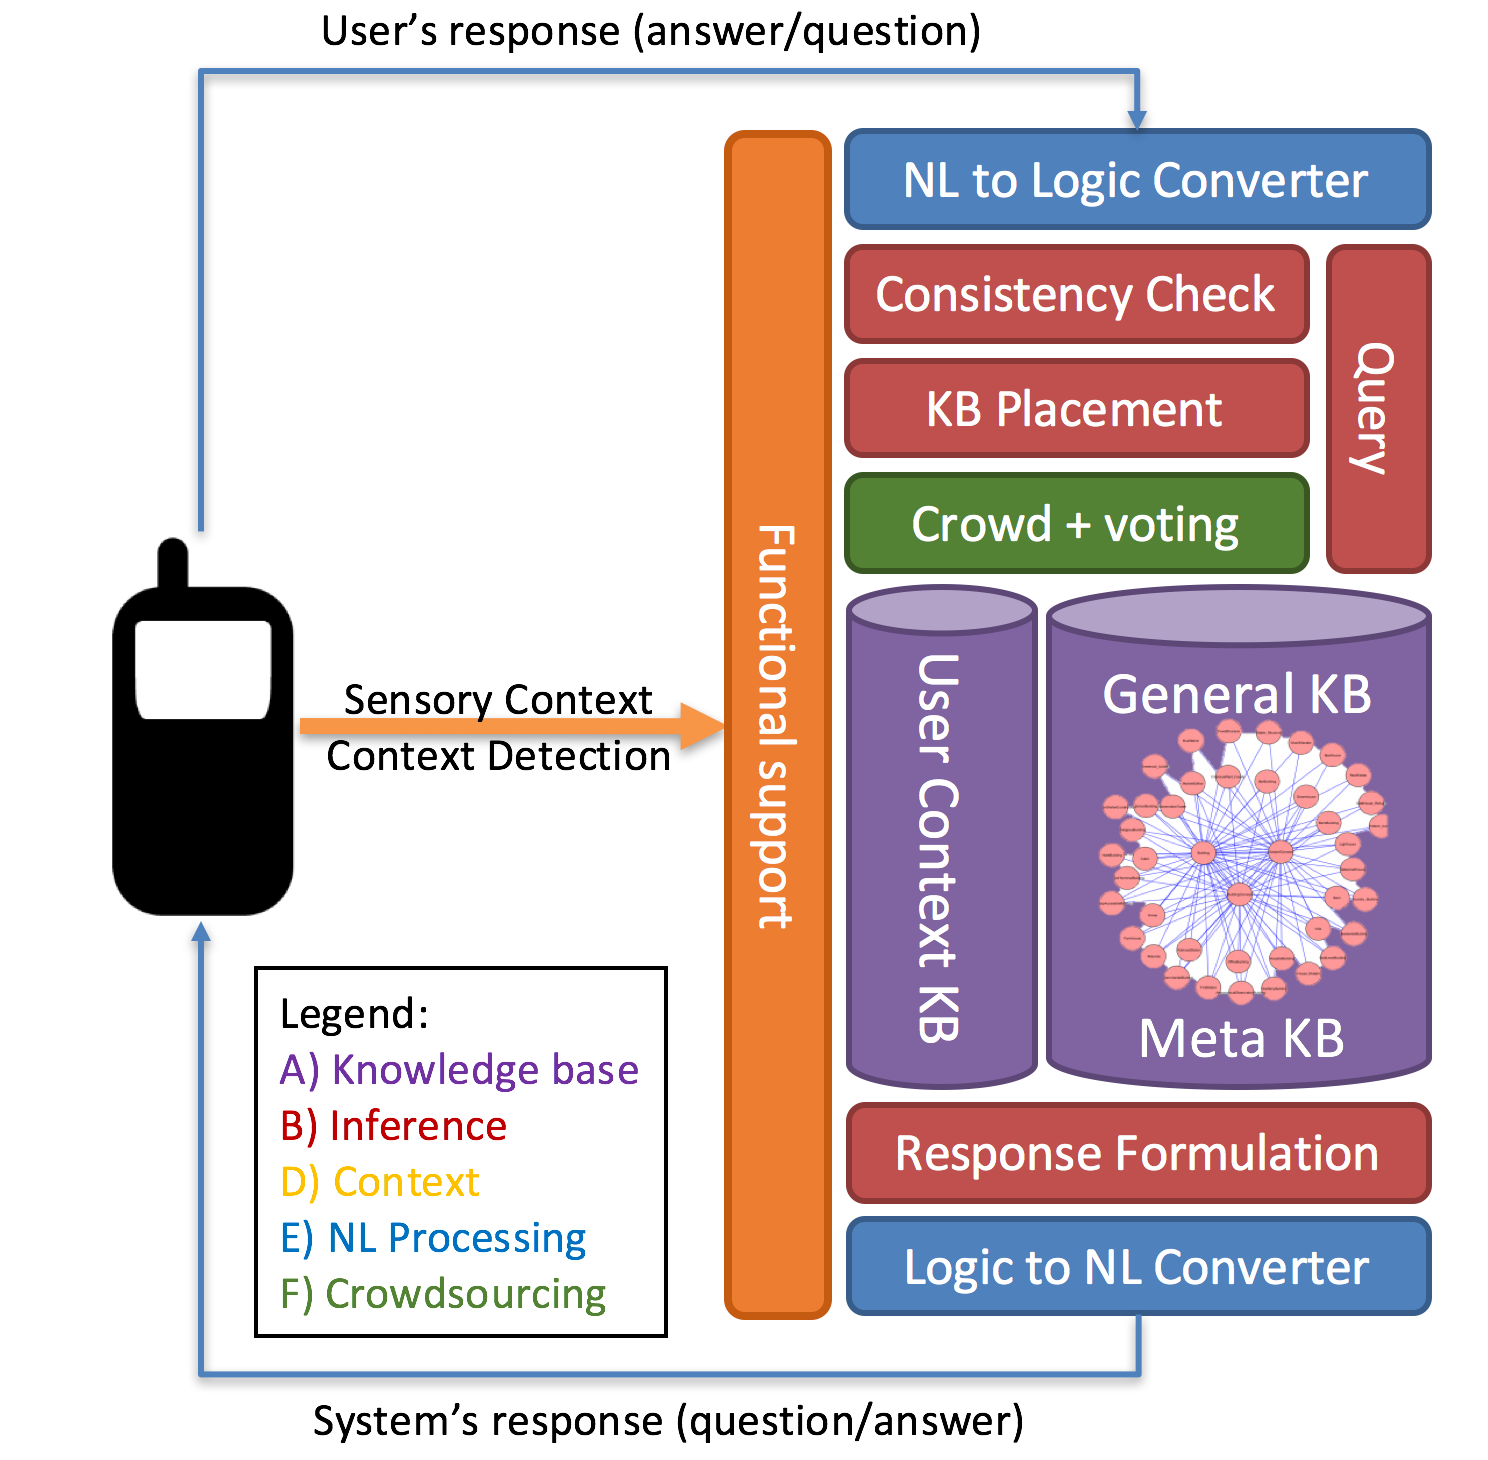
\includegraphics[width=0.9\textwidth]{figures/architecture.png}
	\caption{General Architecture of the KA system, with an interaction loop
			 presented as arrows.}
	\label{fig:Architecture}
\end{figure}

On \autoref{fig:Architecture} these modules are represented with the boxes,
and their functionality groups are presented with the colors (see the figure
legend). Arrows represent the interaction and workflow order and initiation 
(the interaction is initiated/triggered from the origin of the arrow).

We can see that the central core of the
system is the knowledge base (modules marked in purple and letter A). The 
knowledge base consists of \emph{Upper Ontology} gluing everything together, 
\emph{Common Sense Knowledge} to be able to "understand" user's world and check
the answers for consistency, \emph{Meta Knowledge} for enabling inference about 
its internal structures, \emph{User Context KB} to hold current user context and 
\emph{Knowledge Acquisition Rules} to drive the KA process from within the KB, 
using logical inference. 

Next to the KB, is an \emph{Inference Engine} that performs inference over 
the knowledge from the KB. Its modules are represented with the red color 
and letter B. The inference engine needs to be general enough to be able to
perform over full KB, and should be capable of meta-reasoning (over the 
meta-knowledge and KA knowledge in the KB) about the KB's internal knowledge
structures. In cases when the inference engine have some missing functionalities,
some of these tasks can be supplemented by the \emph{Procdeural Support} 
module. In the proposed system, inference engine handles almost all of the 
core KA operations, which can be separated into the following modules:
\begin{itemize}
   \item \emph{Consistency Checking} module which can asses the user's answers
   and check whether they fit within the current KB knowledge.
   \item \emph{KB Placement} module which decides where into the subtree of the
   KB the answer should be placed.
   \item \emph{Querying} module, which employs the inference engine to answer
   questions that are coming from the user through NL to Logic converter.
   \item \emph{Response Formulation} module, which employs the KA meta-knowledge
   and do inference about what to say/ask next. Results of this module are then
   forwarded to the Logic to NL converter and then to the user.
\end{itemize}

Tightly integrated with the knowledge base and inference engine is a 
\emph{Crowdsourcing Module}, which monitors crowd (multipl user's) answers and 
is able to remove (or move to different contexts) the knowledge from the KB, 
based on its consistency among multiple users. If some piece of knowledge inside
the KB is questionable, the module marks it as such and then \emph{Response
Formulation} module checks with other users whether it's true or not and should
maybe be removed or only kept in the one user's part of the KB. This module is 
represented in Green color and letter F.

At the entry and exit point of the system workflow, there are NLP processing  
modules which can convert logic into the natural language and vice versa. These
modules are used for natural language communication with the users. Tese two
modules are represented in Blue and letter E.

On the side of the Figure, there is a procedural module (depicted with Orange
color and letter D), which is a normal software module (in our implementations
written in procedural programming language), which glues everything together.
It contains a web-server, authentication functionalities, machine
learning capabilities, connections to external services and context mining
and other functions that are hard to implement using just logic and inference.
This module is taking care of the interactions between submodules. 

All of the modules are triggered either through the contextual triggers 
(also internal, like when timer detects the specific hour or time of day), or
by the users. When the context changes, it causes the system to use inference
engine to figure out what to do. Usually, as a consequence it results in a 
multiple options like questions or comments. Then it picks one and sends a 
request to the user. This triggering is represented with the arrows, where the 
blue arrows represent natural language interaction, and the orange one
represents structured or procedural interaction, when the procedural module
classifies or detects any useful change in the sensor data sent into the system
py the part running on the mobile phone.

\subsection{Interaction Loop}
\label{section:interaction}
As briefly already mentioned above, besides architecture, 
\autoref{fig:Architecture} also indicates a system/user interaction loop 
represented by arrows. Orange arrow (pointing 
directly from the phone towards the system) represents the automatic interaction
or triggers that the phone (client) is sending to the system all the time. This
provides one part of the user context. After the precedural part analyses
the data (as described in \hl{ref to SPD}) and enter findings into the KB as 
context, this often triggers the system to come up with a new question, or 
context related info. Example of such a trigger is, when user changes a location
and the system figures out the name and type of the new place. On the other 
side, Blue arrows represent the Natural Language interaction which can happen
as a result of automatic context (Orange arrow), or some other reason causing new 
knowledge appearing in the KB. New knowledge can appear as a consequence of
answering a question from the same user, or some other user. This shows, how the
actual knowledge (even if entered automatically through procedural component) is
controlling the interaction, and explains how the system is initialized and how
its main pro-activity driver is implemented. Examples of such initialization
of the interaction is presented in \hl{Script 1 and Script2}. Additionally, the 
user can trigger a conversation at any point in time either by continuing the 
previous conversation or simply starting a new one. 

\begin{figure}[htb]
	\centering
		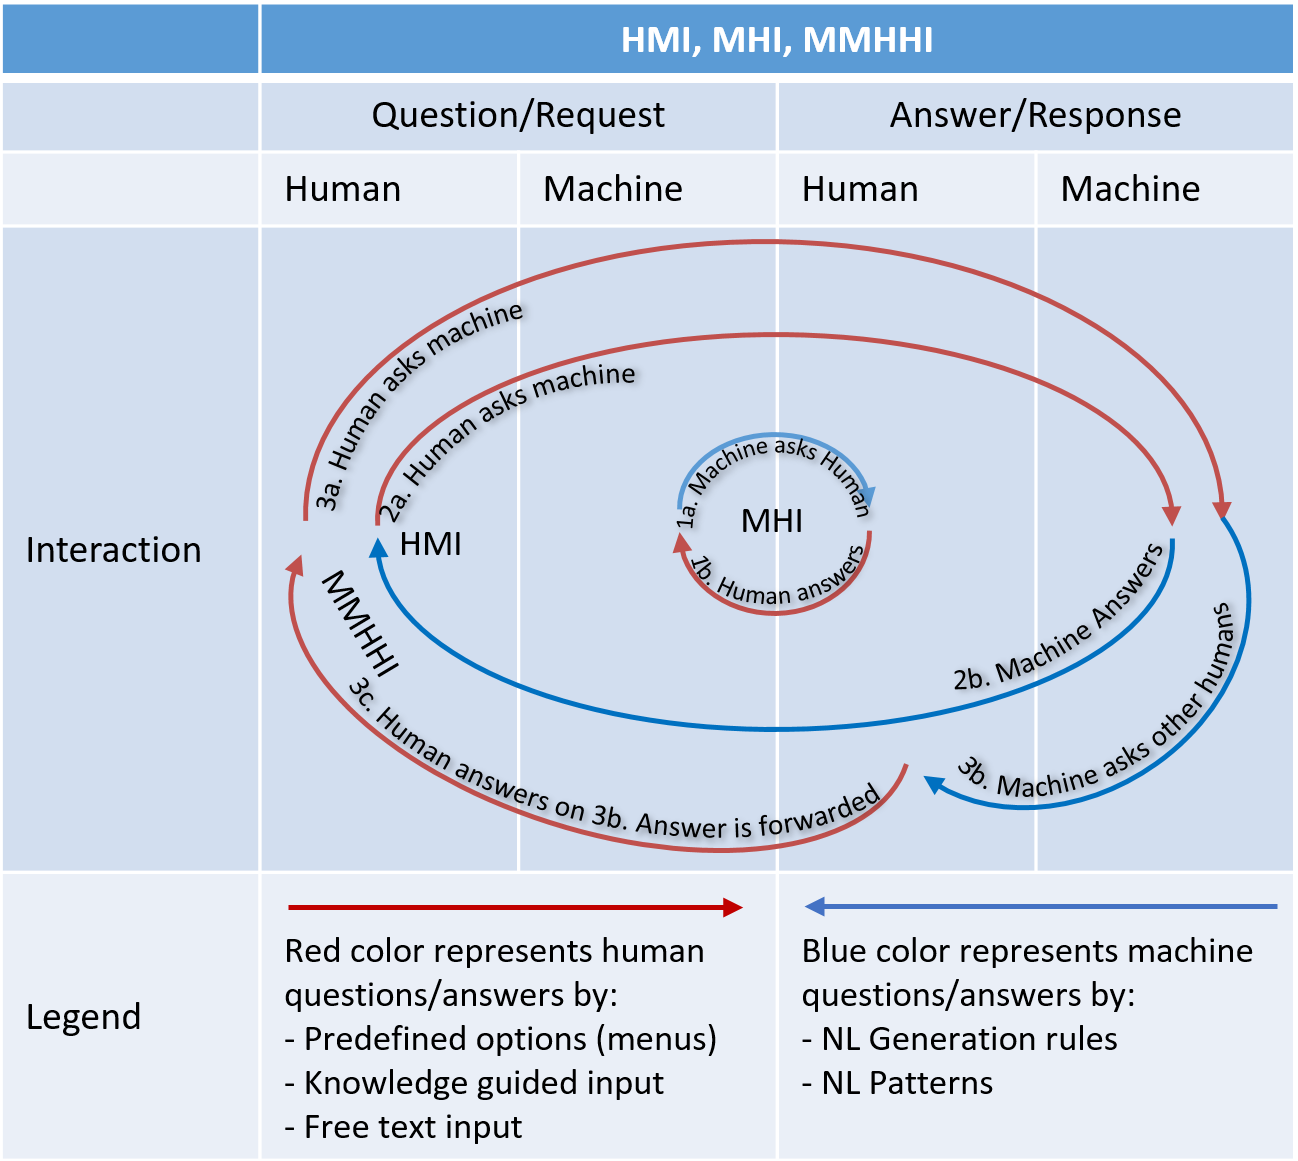
\includegraphics[width=0.9\textwidth]{figures/interactionLoop.png}
	\caption{Possible interaction types between the user and Curious Cat KA
			 System.}
	\label{fig:interaction}
\end{figure}

According to the interactions described above, the proposed KA system have two 
options for the interaction. Human to machine (HMI), when users initiate 
interaction, and machine to human (MHI), when the system initiates the 
interaction. The specifics of both, which cannot fit in 
\autoref{fig:Architecture} are explained in the following sub-sections 
\hl{4.2.1 and 4.2.2}. On top of this, the design of the system allows a novel 
type of interaction which combines multiple users and machine into one 
conversation, while presenting this to the users as a single conversation track
with the machine. This becomes useful when the system doesn't have enough
knowledge to be able to answer user's questions, but it has just enough to know
which other users to ask (i.e. when someone is asking a question about specigic
place and there is no answer in the KB, \emph{Curious Cat} can ask other users
that it knows had been there). This type of the interaction can be called
Machine Mediated Human to Human interaction (MMHHI). This allows the system
to answer questions also when it doesn't know them, while simultaneously also
store and remember the answers, either parsing them and assert them directly to 
KB, or leave them in NL for later Knowledge Mining analysis. The possible
interaction types are also presented on \autoref{fig:interaction}.

\subsubsection{Machine to Human Interaction (MHI)}
\label{section:mhi}
The most basic form of interaction between the CC system and the user, which
we also use the most, is when something triggers a change in the KB and 
CC decides it's the time to ask or tell something. On the 
\autoref{fig:interaction}, this is represented by the most inner loop (MHI). 
Example of this is when the context part of \emph{Procedural} module classifies
a new location and then asserts it into the KB. This then triggers Inference 
Engine which results in a new user query (same as defined in 
\hl{ref to CCWantsToAskLocation}).

\begin{equation*}
	\label{eq:ccWantsLoc}
	ccWantsToAsk(CCUser1, (userLocation(CCUser1,CCLoc1)))
\end{equation*}

This query then goes through logic to NL \hl{ref} conversion, which is then
presented to the user in NL like "Where are we? Are we at the restaurant X?".
This is represented on \autoref{fig:interaction} with a blue arrow on the
inner circle, marked with 1a. The presentation is handled by the client and 
can be in a written form, or through the text-to-speech interface. User can then 
answer this question and thus close the interaction loop (blue arrow marked with
1b), possibly causing a new one with her answer. 

For easier answering, the KA system can use existing KB to generate a set of 
possible answers at the qustion generation time. These can be then picked by
the user instead of writing. THe guidance can consis of variations of these:
\begin{itemize}
	\item A fixed set of pre-defined options that user can pick from, generated
	from the KB.
	\item A set of pre-defined options with an additional free text field when
	the set of possible answers is big or inifite. In this cases the text field
	is connected to the KB providing auto-complete options for valid answers.
	\item Completely free text were user can write anything. This is essentially
	the same as for the HMI interaction described below (\autoref{section:hmi}).
\end{itemize}

The example of mediated answer guidance can be seen in \hl{Fig. 3}, where the 
system presented a set of possible answers while still allowing a free text 
which will be autocompleted with the food types that the system knows about. 
If the user enters something new, the system will accept that (\hl{as was shown 
in the step 6 in Table I)}.

The inference triggering, language rules and mechanisms for context detection
are described in more detail in sections \hl{ref, ref, ref} respectively. This
type of the interaction is where the users answer questions and is thus part of
the main research topic of this thesis.

\subsubsection{Human to Machine Interaction (HMI)}
\label{section:hmi}
The second type of interaction is, when user initiates the conversation. 
If this is done at some point as the answer to an old question, the process is 
the same as described above in \autoref{section:mhi}. But users can also enter a 
free text, asking a question or stating something. In this case, this goes 
through the \emph{NL to Logic Converter} module which tries to convert the
text into logical query or assertion. The complexity of converting NL into logic 
is a lot higher than in the opposite direction, since the language is not
as exact. In CC implementation \hl{ref to CC converter}, we handled this to
some extent by using SCG system \parencite{Schneider2015}, where the text
is matched to NL patterns which are linked to appropriate logical structures.
\hl{This would be used for example, when user, instead of simple Pizza Deluxe 
(step 5 in Table I), would say They sell pizzas or something even more complex 
(see section 4.5.2)}. After the text is converted into logic, inference engine 
can use it to query it against the KB, and show the answers back to user, again 
converted into NL through \emph{Logic to NL Converter} module. This type of
interaction is depicted on \autoref{fig:interaction} by the middle arrow circle
started by humans (arrow 2a), where machine provides the response (arrow 2b).

%SUBSECTION
\subsubsection{Machine Mediated Human to Human Interaction (MMHHI)}
\label{section:mmhhi}
Both of the interactions described in sections \ref{section:mhi} and 
\ref{section:hmi} pre-supposes that the receipient of the query, knows how to
answer it, or respond otherwise. In the cases when, let's say machine doesn't
have any answer (The NL question gets converted into the logical query, which doesn't retrieve any aswers from within the KB). It could respond with 
"I don't know", which is a valid response.
Thile this allows for the conversation to continue, it doesn't help the user
to get the answer, also does not benefit to knowledge acquisition. The only 
thing the system can learn from this, is that user is interested in the object
of the question. This doesn't have to end there though, since CC has access to
other users and knowledge about their past and current contexts. Based on the
topic of interes from the user query, the system can easily find users which
might know the answer (inferred from their past whereabouts, answers, etc.).
Once such an user is deteced, the original question can simply be forwarded to
him, as it would be asked by CC itself. Once he, or one of the users answers,
CC can forward it to the original user. On top of that, CC can parse the answer
the same way as described above for HMI and MHI (sections \ref{section:mhi},
\ref{section:hmi}), and remember it, placing it into the KB. In the cases when
the language of the answer is too complex, it can be stored in its original
format, for later text-mining apporach which can lead to learning of new-patterns
as well as the knowledge hiding in the answers. On top of this, CC can also
remember the question itself, and place it on specific type of concepts, as an
important quetsion to ask. On \autoref{fig:interaction},
MMHHI approach is depicted by the outer circle of arrows, where 3a is original 
user's question, which is forwarded to other users when CC doesn't know how to 
answer (3b). After one or more of the users answer, the answer is forwarded back
to the original user (3c).

%SECTION
\section{Knowledge Base}
\label{section:kb}
As visible in \autoref{fig:Architecture}, Knowledge Base is the central part
of the proposed KA system. Internally KB has three components. The main part, 
which should in any real implementation of the system also be the biggest, is 
the common-sense knowledge, and its upper ontology over which we operate. 
This part of the system contributes the most to the ability to check the 
answers for consistency. The more knowledge already exists, the easier becomes 
to assess the answers, come up with new questions and also propose possible
answers in the guided interaction(\hl{ref}).

The second part is the user Context KB, which stores the contextual knowledge 
about the user. This covers the knowledge that the user has provided about 
himself (\hl{ref}) and the knowledge obtained by mining raw mobile sensors 
(\hl{ref}). On \autoref{fig:Architecture}, This part of the KB is represented 
as the left-most KB, sitting between the main KB and the 
\emph{Procedural Module}.The sensor based context allows the system to 
proactively target the right users at the right time and thus improve the 
efficiency and accuracy and also stickiness of the KA process.

The third KB part, is the meta-knowledge and KA rules that drive the dialog and 
knowledge acquisition process (\hl{ref}). Although in our implementation we 
used Cyc KB (\hl{ref} and also tested Umko KB (\hl{ref}), the approach is not 
fixed to any particular knowledge base. But the KB needs needs to be expressive
enough to be able to cover the intended knowledge acquisition tasks and 
meta-knowledge needed for the system's internal workings. 

Because the full Curious Cat system including the KB is too big and complex to 
be fully explained here (the KA Meta Knowledge alone consists of 12,353 
assertions and rules), we will focus on the fundamentals of the idea and 
approach, and define the simplest possible logic to explain the workings 
through the examples given in the \hl{ref} and  \hl{ref Table II}. 

The logic examples are given in formal higher order predicate logic, which we 
later replace with a more compact notation, with a slight change in the way the 
variables are presented. For better readability, instead of $x, y, z$, we mark 
variables with a question mark ($?$) followed by a name that represents the 
expected type of the concepts the variable represents. For example, when we see 
a variable in a logical formula like $CCUser(?PERSON)$, we immediately know that
$?PERSON$ can be only replaced with (bound to) instance or subclasses of the 
concept $Person$. We start predicate names with a small letter 
($predicate$) and the rest of the 
concepts with a capital letter ($Concept$). At this point it is worth noting 
that while our logical definitions and formalization are strongly influenced by 
Cyc\parencite{Lenat1995}, and while the approach is based on the Cyc upper 
ontology, the approach is general and not bound to any particular 
implementation, and our notation below reflects but is not tightly bound to 
that of OpenCyc. \todo{Add footnotes as in the paper}

%SUBSECTION
\subsection{Upper Ontology}
\label{section:upperOnto}
First we introduce the vocabulary or terms (constants/concepts) that will allow 
us to construct the upper ontology which is the glue of any knowledge base that 
can be used for machine inference:

\begin{equation}\label{set:terms}
\begin{gathered}
S_{Constants} = \{Something, Class, Number, Predicate, subclass, \\
	is, arity, argClass, argIs\}
\end{gathered}
\end{equation}

In the standard \emph{predicate logic}, $P(x)$ notation tells us that whathever 
the $x$ stands for, it has the property defined by the predicate $P$. 
For example, the following propositional function:

\begin{equation}\label{eq:examplepred}
Person(x)
\end{equation}
is stating that something ($x$) is a person, or more precisely, $x$ is an 
instance of a class $Person$. In order to be able to construct logical 
statements ranging
over classes and their instances in a more controlled and transparent way, we
use a constant $is$, and define it as a predicate denoting that something is an
instance of some class.

\begin{definition}[predicate "$is$"]
\label{const:is}
Predicate $is(x,y)$ denotes that $x$ is an instance of $y$. For example, 
stating $is(John, Human)$ defines John as one instance of the class of humans.
\end{definition}
Now, to make things clearer and more precise, instead of writing instance
relation through custom predicate $Person(x)$, we can use more precise syntax, 
which allow us to specify what is instance of which class: $is(x,Person)$.

As visible in the \autoref{eq:examplepred}, in predicate logic, predicates are
defined only with usage. Everything that we write as a predicate in a similar
formula is then defined as a predicate. This is not a desired behavior in our 
KA approach, since the knowledge will be coming from the users with various
backgrounds and without any idea of predicate logic. For this reason we
need more control of what can be used where, if we want to be able to
check for consistencies and have control of our KB with the inference engine.
For this reason, we enforce a constraint (rule).

\begin{definition}[Predicate Constraint]\label{constraint:predicate}
Everything that we want to use in the KB as a predicate, must first be defined
as an instance of the $Predicate$ class:
$\forall x \in S_{Predicates}: is(x,Predicate)$. From the other side, set of
predicates can be defined as $S_{Predicates}=\{x:is(x,Predicate)\}$.
This constraint can be inserted into our KB as a \emph{material implication}
rule, which needs to be true at all times, to serve as a constraint:
\begin{equation}\label{rule:pred_constraint}
\forall P \forall x_{1...n} (P(x_1...x_n) \implies is(P,Predicate))
\end{equation}
\end{definition}

Now, careful reader might notice, that we actually cannot use $is$ as a 
predicate, since nowhere in our KB is stated that this is actually a 
predicate. To fix this error and make our KB consistent with its constraints,
we need to add an assertion defining what term $is$ stands for:

\begin{equation}\label{as:is_is}
is(is, Predicate)
\end{equation}
At the time the above assertion (Assertion \ref{as:is_is}) is asserted
into the KB, it also becomes valid assertion, since it complies with the
constraint defined in Definition \autoref{constraint:predicate} and thus our
Constraint Rule \ref{rule:pred_constraint} is true. After this 
assertion is in the KB, $ir$ can be used as a predicate because it is an 
instance of the term $Predicate$ and complies with our constraints. 

At this point we can define(assert) the rest of our predicates:

\begin{equation}\label{as:predicates}
\begin{gathered}
is(subclass, Predicate) \land is(arity,Predicate) \land is(argClass,Predicate)\\
\land is(argIs,Predicate)
\end {gathered}
\end{equation}
And also the rest of our terms, which we define as instances of term $Class$.
\begin{equation}\label{as:is_class}
\begin{gathered}
	is(Class,Class) \land is(Predicate,Class)\\ 
\land is(Number, Class)
\end {gathered}
\end{equation}

In Predicate logic, predicates have a property called arity, which defines 
number of arguments that the predicate can have. For example, if predicate
$P$ has arity of 1, then it can only take one operand (variable or term). In 
this case only $P(x)$ or $P(a)$ are valid statements, and $P(x,y)$ is not.
In our KB, arity is defined using $arity$ predicate, which itself was defined
in Assertion \ref{as:predicates}.

\begin{definition}[predicate "$arity$"]\label{def:arity}
Predicate $arity(x,y)$ denotes that predicate $x$ has arity of $y$.
\end{definition}

Similarly, as with the constraint that all predicates need to be defined as
such (Definition \autoref{constraint:predicate}), we gain more control over 
KB and make things easier for the inference engine and KA approach, if we 
limit the assertions, to "obey" the predicate arities. For this reason our KB
has additional constraint.

\begin{definition}[Arity Constraint]\label{constraint:arity}
All assertions in CC KB are valid only, when the predicates used in the 
assertion have the same number of arguments as defined with their $arity$ 
assertions:
\begin{equation}\label{rule:arity_constraint}
\forall P \forall n \forall x_{1...n}:(P(x_1,...,x_n) \implies arity(P,n))
\end{equation}
\end{definition}

After we add the above rule (Constraint Rule \ref{rule:arity_constraint}), our 
KB is not consistant anymore, since all the $is(x,y)$ assertions (Assertions 
\ref{as:is_is}, \ref{as:predicates}) violate the constraint. We fix this by 
adding the following assertion:

\begin{equation}\label{as:arity_is}
arity(arity,2) \land arity(is,2)
\end{equation}
This makes the KB consistant again, because we defined all the arities of
predicates $arity$ and $is$, which we have used so far in our KB, as well as 
defined them with $is(x, Predicate)$ assertions. We can now continue with 
defining the arities of the rest of the predicates:

\begin{equation}\label{as:arity_predicates}
\begin{gathered}
arity(subclass, 2) \land arity(argClass,3) \land arity(argIs,3)
\end {gathered}
\end{equation}
We can see now that the arity of $is$ predicate is defined as 2 (same as for 
$subclass$ and $arity$, which can be used to define arity of itself), and can 
confirm that all the logical formulas in the definitions up to now are correct.

To be able to describe the world in more detail, we define the $subclass$ 
predicate, which handles the hierarchy relations between multiple classes 
(unlike $is$, which handles relationships between classes and their instances).

\begin{definition}[predicate "$subclass$"]\label{def:pred_subclass}
Predicate $sublcass(x,y)$ denotes that $x$ is a subclass of $y$. For example, 
asserting $subclass(Dog, Animal)$, is specifying all dogs, to be a sub-class of
animals, and $subclass(Terrier,Dog)$ is speficfying that all terriers are 
sub-class of dogs. At this point we might notice that while it is logical to us
that terriers are also a sub-class of animals, there is no way for the machine
inference to figure that out. For this reason we need to introduce a
"subclass transitivity" inference rule:
\begin{equation}\label{rule:subclass_transitivity}
\begin{gathered}
  \forall x \forall y \forall z: ((subclass(x,y) \land subclass(y,z)) \implies subclass(x,z))
\end{gathered}
\end{equation}
The rule above is basically saying that if a first thing is a sub-class of a
the second thing, and then thesecond thing is a subclass of the thirdthing,
then the third thing is a sub-class of the first thing as well. 
\end{definition}

Because we want to be able to prevet our system from acquiring incorrect 
knowledge, we need to limit the domains and ranges of the predicates 
(arguments). This could be done by adding a speciic constraint rules
(material implication rule without the power to make new assertions). For 
example, for both $subclass$ arguments, to only allow instances of a $Class$, 
we could assert:
\begin{equation}\label{as:domain_example}
  \forall x_1 \forall x_2: (subclass(x_1,x_2) \implies (is(x_1,Class) \land 
  is(x_2,Class))
\end{equation}
Because the rule (Rule \ref{as:domain_example} is only true if the right part
(the consequent) is true, or the left part (the antecedent) is false, its
inclusion in the KB (as with other constraint rules) forces the KB to not allow
the arguments of subclass to be anything else than an instance of a class 
$Class$. It would be hard to construct a large KB, by writing the rule
like this for each of the thousands potential predicates. To make this easier,
following Cyc practice\parencite{Lenat1995}, we will introduce $argIs$ 
predicate (Definition \ref{def:pred_subclass}). To make this definition more understandable, let's
first expand the example (Rule \ref{as:domain_example} above:

\begin{equation}\label{as:domain_ext_example}
\begin{gathered}
  \forall x_1 \forall x_2: (subclass(x_1,x_2) \implies (is(x_1,Class) \land is(x_2,Class)) \\ 
  \iff \\
  argIs(subclass,1,Class) \land argIs(subclass,2,Class))
\end{gathered}
\end{equation}
This rule above (Rule \ref{as:domain_ext_example} states, that the constraint
rule (Rule \ref{as:domain_example} can be written as 2 $argIs$ assertions.
Instead of writing full rule, the constraint for the argunent of $subclass$ can
be written simply as $argIs(subclass,1,Class)$. To make this hold for all the
combinations of predicates (not just $subclass$ from example), we can
re-phrase the rule to be general, and also define the $argIs$ predicate.

\begin{definition}[predicate "$argIs$"]\label{def:pred_argis}
Predicate argIs(x,y,z) denotes that the $y-th$ argument of predicate $x$, must
be an instance of $z$. For example, asserting \\$argIs(subclass,1, Class)$, states
that the first argument of predicate $subclass$ must be an instance of $Class$.
This is enforced by the following constraint rule:
\begin{equation}\label{as:domain_isa_constraint}
\begin{gathered}
  \forall P \forall n \forall x_1...x_n \forall C_{1...m}: \\
  ((arity(P,n) \land P(x_1,...,x_n)) \implies (is(x_1,C_{1...m}) \land ... \land is(x_n,C_{1...m})) \\ 
  \iff \\
  argIs(P,1,C_{1...m}) \land ... \land argIs(P,n,C_{1...m}))
\end{gathered}
\end{equation}
\end{definition}

These definitions allow us to use simple $argIs$ assertions, instead of
complicated rules. For the cases, when the arguments shouldn't be instances
of a $Class$, but its subclasses, we can define similar predicate and its
constraint rules also fro $argClass$:

\begin{definition}[predicate "$argClass$"]\label{def:pred_argClass}
Predicate $argClass(x,y,z)$ denotes that the $y-th$ argument of predicate $x$, 
must be a subclass of $z$. For example, asserting 
\\$argClass(servesCuisine, 2, Restaurant)$, states that the first argument of 
predicate $servesCuisine$ must be a subclass of $Restaurant$.
This is enforced by the following constraint rule (similar as for $argIsa$, but
for $argClass$):
\begin{equation}\label{as:domain_class_constraint}
\begin{gathered}
  \forall P \forall n \forall x_1...x_n \forall C_{1...m}: \\
  ((arity(P,n) \land P(x_1,...,x_n)) \implies (subclass(x_1,C_{1...m}) \land ... \land subclass(x_n,C_{1...m})) \\ 
  \iff \\
  argClass(P,1,C_{1...m}) \land ... \land argClass(P,n,C_{1...m}))
\end{gathered}
\end{equation}
\end{definition}

Before we can assign argument constraints to our existing predicates and have
all the KB valid, we need to define a special class $Number$:

\begin{definition}[class $Number$ and its instances]\label{def:number}
All natural numbers are instances of the class $Number$. Formally, this can be
asserted into a KB as:
\begin{equation}\label{as:numbers}
	\forall x \in \mathbb{N}:is(x,Number)
\end{equation}
\end{definition}

This now allows us to use $argIs$ and $argClass$ predicates instead of 
complicated rules, to define types of arguments inside any predicate used in the
KB. By using these two newly defined predicates, we can now proceeed to assert 
the argument limits of the $argIsa$ predicate itself: 

\begin{equation}\label{as:argIs_domain}
\begin{gathered}
argIs(argIs,1,Predicate) \land argIs(argIs,2,Number) \land argIs(argIs,3,Class) 
\end{gathered}
\end{equation}
We can see that the first argument must be an instance of $Predicate$, which 
holds in all three cases ($argIs$ is a first argument of the Assertion 
\ref{as:argIs_domain} above), since it was defined in Assertion 
\ref{as:predicates}. Similary, the second argument is a valid number, in all 
three cases as defined in Definition \ref{def:number}. Also the third arguments
($Predicate$, $Number$,$Class$), are all instances of the $Class$ as defined in
Assertion \ref{as:is_class}, so the assertion \ref{as:argIs_domain} can be asserted
and it doesn't invalidate itself throigh argument contraint rule (Constraint 
\ref{as:domain_isa_constraint}).

Similary, we can now proceed to define the rest of our predicates. Starting with
the most similar $argClass$:
\begin{equation}\label{as:argClass_domain}
\begin{gathered}
	argIs(argClass,1,Predicate) \land argIs(argClass,2,Number) \\
	\land argIs(argClass,3,Class) 
\end{gathered}
\end{equation}
Since we didn't yet assert any direct $argClass$ constraint, this predicate
at this point defines the constraints, without any danger to invalidate our
current KB. 

Continuing with $subclass$. On the Definition \ref{def:pred_subclass}, 
we can see that this
predicate defines sub-class relationships between the classes. For this reason
it makes sense to only allow instances of $Class$ for its arguments:
\begin{equation}\label{as:subclass_is_constraint}
	argIs(subclass,1,Class) \land argIs(subclass,2,Class)
\end{equation}
Same as with the Assertion \ref{as:argClass_domain}, we didn't yet assert any 
direct assertions about something being a sub-class of something, this assertion
doesn't affect yet the validity of our KB, while prevents future assertions of 
$subclass$ predicate on anything but $Class$ instances.

For the $arity$ predicate, we can check our existing assertions 
(\ref{as:arity_is}, \ref{as:arity_predicates}), and
see that as the first argument we always have an instance of $Predicate$, while
as the second argument we have an instance of a $Number$. According to this, it
serves our purpose and is safe to limit the arguments of $arity$ to:
\begin{equation}\label{as:arity_is_constraint}
	argIs(arity,1,Predicate) \land argIs(arity,2,Number)
\end{equation}

We can now proceed to define our last ($is$) predicate constraints, which is
a bit more complicated. If we look at our existing  $is$ assertions 
(\ref{as:is_is}, \ref{as:predicates}, \ref{as:numbers}), we can
see that as a second argument we always have an instance of a $Class$ 
($Predicate$, $Class$), but
for the first argument we can actually put in anything ($is$, $Class$, 
$Predicate$,  $Number$, $\mathbb{N}$). From instance of a $Class$,
instance of a $Predicate$, to an instance of a $Number$. For the second argument
we can imediatelly asert

\begin{equation}\label{as:is_arg2_domain}
argIs(is,2, Class)
\end{equation}

In order to be able to say that some argument can be anything, we followed a 
Cyc example and introduce term $Something$, first mentioned in the set of our 
terms in Assertion \ref{set:terms}. We set this as the constraint for the first
argument of $is$ predicate:

\begin{equation}\label{as:is_arg1_domain}
argIs(is,1, Something)
\end{equation}
But this assertion above (\ref{as:is_arg1_domain}), invalidates the correctnes
of all of our $is$ assertions, since none of the current first arguments are
instances o $Something$ (see Assertions \ref{as:is_is}, \ref{as:predicates} and 
\ref{as:numbers}). To fix this, we need to be able at least to say that things 
are instances of $Something$ ($is(x,Something)$). According to the $is$ argument
constraint assertion above (\ref{as:is_arg2_domain}), $Something$ must be an 
instance of a $Class$. So we define it as so:

\begin{equation}\label{as:is_something}
	is(Something,Class)
\end{equation}
Now, as a consequence of this, we could assert for all of the arguments that
are used in $is$ ($is$, $Class$, $Predicate$, $Number$, $\mathbb{N}$), that 
they are an instances of the $Something$. This would
be highly unpractical, since we would need to do this for every future constant
to be used by $is$ predicate (especially unpractical for infinite number of
$\mathbb{N}$).

Instead, since we know that $Something$ is an instance of a $Class$, we can use 
it in our $subclass$ assertions (a consequence of constraint Assertion 
\ref{as:subclass_is_constraint}) and state that $Class$ is a subclass of 
$Something$:
\begin{equation}\label{as:subclass_something}
	subclass(Class, Something)
\end{equation}
A consequence of this assertion is (because of inference rule 
\ref{rule:subclass_transitivity}), that
every sub-class of anything that exists in our KB (because we can only use 
instances of $Class$ in $subclass$ assertions), is a sub-class of $Something$ as
well. This doesn't yet seem to help us make our 1st $is$ predicate arguments 
instances of $Something$, but it will, after we address another weaknes in our
current KB. 
Consider the continuation of the example we started in $subclass$ 
definition (Definition \ref{def:pred_subclass}, where a terrier is a sub-class
of dog, and dog is a sub-class of animals ($subclass(Dog,Animal)$, 
$subclass(Terrier,Dog)$). If we introduce an instance of the
class $Terrier$, let's say, a real dog named "Spot" ($is(Spot,Terrier$)), we can
see that there is a logical problem, since Spot is a terrier in our KB, but
not a dog, or even an animal (there is nothing to support $is(Spot,Animal)$ 
assertion. This can be fixed by introducing the following Inference Rule:

\begin{equation}\label{rule:is_transfer}
\begin{gathered}
  \forall x \forall y \forall z: ((is(x,y) \land subclass(y,z)) \implies is(x,z))
\end{gathered}
\end{equation}
This rule is basically saying, that if there is an instance of a class, and this
class is a sub-class of another class, then this instance is also an instance of
the other class. Now, this inference rule (\ref{rule:is_transfer}), together 
with the fact that $Class$ is a sub-class of $Something$, and the $subclass$
transitivity inference rule (\ref{rule:subclass_transitivity}), makes everything
 that is instance of a 
class, or its sub-class (which is everything in our KB), also an instance of
$Something$, and thus proving the assertion \ref{as:is_arg1_domain} correct and 
consequently our KB fully consistant again.

At this point our Upper Ontology is defined (it is visually presented on
\autoref{fig:upperOnto}) and ready to build upon as will be
described in the next chapters. Since Curious Cat main implementation is based
on Cyc, and it was inspired by the way Cyc ontology is constructed and being 
used, this upper ontology reflects the main part of Cyc upper ontology 
(see Chapter \ref{chapter:implementation}, implementation on how this 
formalization maps to Cyc). While our upper ontology logical definitions and 
formalizations are strongly influenced by Cyc, the approach is general and not 
bound to any particular implementation, and our notation reflects but is not 
tightly bound to that of Cyc. For example, the usage of $argIs$ and $argClass$
can be replaced by $domain$ and $range$ when using a RDF schema, such as was 
done in our RDF prototype implenentation\parencite{Bradesko2012a}, or a 
completely custom constraints can be used in specific ontologies, so this
upper ontology is more of a guidence and a tool to be able to explain apporach,
than a fixed ontology that needs to be implemented.

\begin{figure}[H]
	\centering
		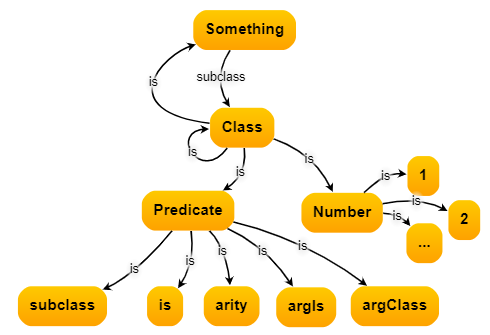
\includegraphics[width=0.8\textwidth]{figures/upperOntology.png}
	\caption{Upper ontology terms, with 'is' and 'subclass' relations.}
	\label{fig:upperOnto}
\end{figure}


%SUBSECTION
\subsection{Existing Knowledge}
\label{section:existingKB}
This sub-chapter extends our upper ontology example with additional knowledge
that allows us to explain the system through the examples given in 
\autoref{tab:conversation1} and \autoref{tab:conversation2}. 

As also visible in the Architecture schematic (\autoref{fig:architecture},
KB with background knowledge is one of the most crucial elements of proposed 
approach. It serves both, as the driving force behind the source of the 
questions, since with the help of contextual knowledge triggers the infrence to
produce logical queries for the missing parts of the knowledge. At the same time
it is the drive behind the proactive user interaction, sarting either as a
question or a suggestion. Finally, the background knowledge is also used for 
validation of answered questions. If the answers are not consistent according
to the existing KB, users are required to re-formulate, or repeat the answer.

The main \emph{Curious Cat} implementation, uses an extended 
full Cyc ontology and KB, similar to that released as ResearchCyc, as a 
common sense and background knowledge base. This is far too big (millions of 
assertions), to be explained in any detail here with the general approach (it 
is explained in more detail in Chapter \ref{chapter:implementation}, 
Implementation). In this chapter we define only the concepts and predicates 
and thus construct the minimal example KB that is necessary for explaining the p
roposed system.

First we introduce the set of new concepts that we need for the food part
of the ontology. These concepts are defined on top of the existing Upper 
Ontology, so the new parts of the KB should maintain the consistency of the
already described parts. The set of terms $S_{Food} $, needed to describe this 
part of the KB is as follows:

\begin{equation}\label{set:foodTerms}
\begin{gathered}
S_{Food} = \{FoodOrDrink,Food,Bread,Baguette,Drink,Coffee\}
\end{gathered}
\end{equation}
Where each of these terms is an instance of a $Class$:
\begin{equation}\label{set:foodTermsClass}
\begin{gathered}
\forall x \in S_{Food}: isa(x,Class)
\end{gathered}
\end{equation}
Then, these classes are connected into a class-hierarchy, which is done with
a $subclass$ predicate:

\begin{equation}\label{as:kbFoodSubclasses}
\begin{gathered}
    subclass(Drink,FoodOrDrink) \land subclass(Coffee,Drink) \land \\
	subclass(Food,FoodOrDrink) \land subclass(Bread,Food) \land \\
	subclass(Baguete, Bread)
\end{gathered}
\end{equation}
Which is also presented graphically on \autoref{fig:foodSubclass} below.
\begin{figure}[H]
	\centering
		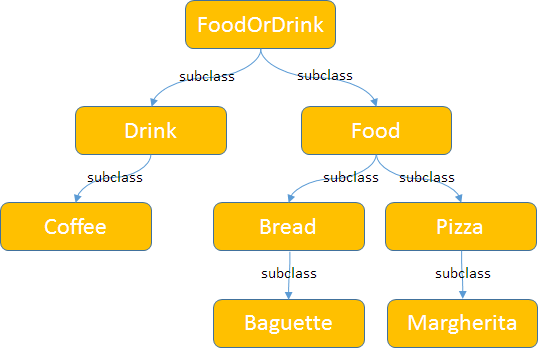
\includegraphics[width=0.6\textwidth]{figures/foodOntology.png}
	\caption{Hierarchy of food related terms, specified by subclass predicates.}
	\label{fig:foodSubclass}
\end{figure}

The second part of ontology (KB) constructing knowledge about places consist
of the following terms:

\begin{equation}\label{set:placeTerms}
\begin{gathered}
S_{Place} = \{Placa,PublicPlace,PrivatePlace,Restaurant\}
\end{gathered}
\end{equation}
Where each of these terms is also an instance of a $Class$:
\begin{equation}\label{set:placeTermsClass}
\begin{gathered}
\forall x \in S_{Place}: isa(x,Class)
\end{gathered}
\end{equation}
Then, these classes are connected into a class-hierarchy, which is done with
a $subclass$ predicate:

\begin{equation}\label{as:kbPlaceSubclasses}
\begin{gathered}
    subclass(PrivatePlace,Place) \land subclass(PublicPlace,Place) \land \\
	subclass(Restaurant,PublicPlace) \land subclass(Home,PrivatePlace)
\end{gathered}
\end{equation}
Which is also presented graphically on \autoref{fig:placeOntology} below.
\begin{figure}[H]
	\centering
		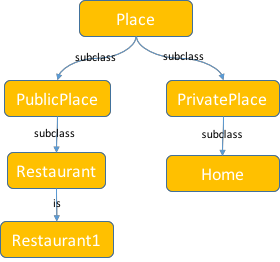
\includegraphics[width=0.6\textwidth]{figures/placeOntology.png}
	\caption{Hierarchy of place related terms, specified by subclass predicates.}
	\label{fig:placeOntology}
\end{figure}

Then the last part (excluding predicates which are defined separately),
of our \emph{Existing Knowledge} consist of the following terms:

\begin{equation}\label{set:otherTerms}
\begin{gathered}
S_{Reest} = \{Service,WirelessService,Vehicle,Car,Animal,Duck,\\
	Human,User\}
\end{gathered}
\end{equation}
Where each of these terms is also an instance of a $Class$:
\begin{equation}\label{set:restTermsClass}
\begin{gathered}
\forall x \in S_{Rest}: isa(x,Class)
\end{gathered}
\end{equation}
And a class-hierarchy:

\begin{equation}\label{as:kbPlaceSubclasses}
\begin{gathered}
    subclass(Car,Vehicle) \land subclass(WirelessService,Service)\land\\
	subclass(Duck,Animal)\land subclass(Human,Animal)\land \\
	subclass(User,Human)
\end{gathered}
\end{equation}
Which is also presented graphically on \autoref{fig:restOntology} below.
\begin{figure}[H]
	\centering
		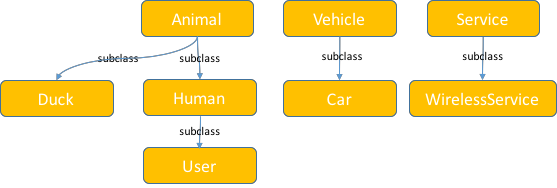
\includegraphics[width=0.9\textwidth]{figures/restOntology.png}
	\caption{Hierarchy of the rest of the terms from our \emph{existing 
	knowledge.}}
	\label{fig:restOntology}
\end{figure}
We can see that all these new terms add on top of the existing set of terms from 
upper ontology ($S_{Constants} = S_{upper} \cup S_{Food} \cup S_{Place} 
\cup S_{Rest}$). 

For defining the predicates, we need a bit more detailed definitions, since we 
also want to represent the constraints which will serve for the inference 
engine to check the validity of the answers (as explained in 
\hl{ref to constraints def. in UpperOnto}).

\begin{definition}[predicate $menuItem$]\label{def:menuItem}
Predicate $menuItem(x,y)$ denotes that place $x$ has a menu item $y$ on its 
menu.Formally it is defined as:
\begin{equation}\label{as:pred_menuItem}
\begin{gathered}
    is(menuItem,Predicate) \land \\
	argIs(menuItem,1,Restaurant) \land\\
	argClass(menuItem,2,FoodOrDrink)
\end{gathered}
\end{equation}
\end{definition}
As we see defined above (assertion \ref{as:pred_menuItem}), this predicate
constraints allow us to only use instances of class $Restaurant$ for the first
argument, and sub-classes of class $FoodOrDrink$ for the second. Besides the 
items on the menu, to explain our examples, we also need a way to tell that
a place provides some services.

\begin{definition}[predicate $providesServiceType$]\label{def:serviceType}
Predicate $providesServiceType(x,y)$ denotes that place $x$ provides service 
$y$. Formally it is defined as:
\begin{equation}\label{as:providesServiceType}
\begin{gathered}
    is(providesServiceType,Predicate) \land \\
	argIs(providesServiceType,1,Place) \land\\
	argClass(providesServiceType,2, Service)
\end{gathered}
\end{equation}
\end{definition}
As defined in the Assertion \ref{as:providesServiceType}, $providesServiceType$
constraints allow us to only use instances of class $Place$ (Public,Private,
Home,Restaurant for the current stage of the KB) for the first argument, and 
sub-classes of class $Service$ for the second. 

\begin{definition}[predicate $userLocation$]\label{def:userLocation}
Predicate $userLocation(x,y)$ denotes that user $x$ is located at place 
$y$. Formally it is defined as:
\begin{equation}\label{as:userLocation}
\begin{gathered}
    is(userLocation,Predicate) \land \\
	argIs(userLocation,1,User) \land\\
	argIs(userLocation,2, Place)
\end{gathered}
\end{equation}
\end{definition}
As defined in the Assertion \ref{as:userLocation}, $userLocation$
constraints allow us to only use instances of class $User$ for the first
argument, and instances of $Place$ as a second.

\begin{figure}[H]
	\centering
		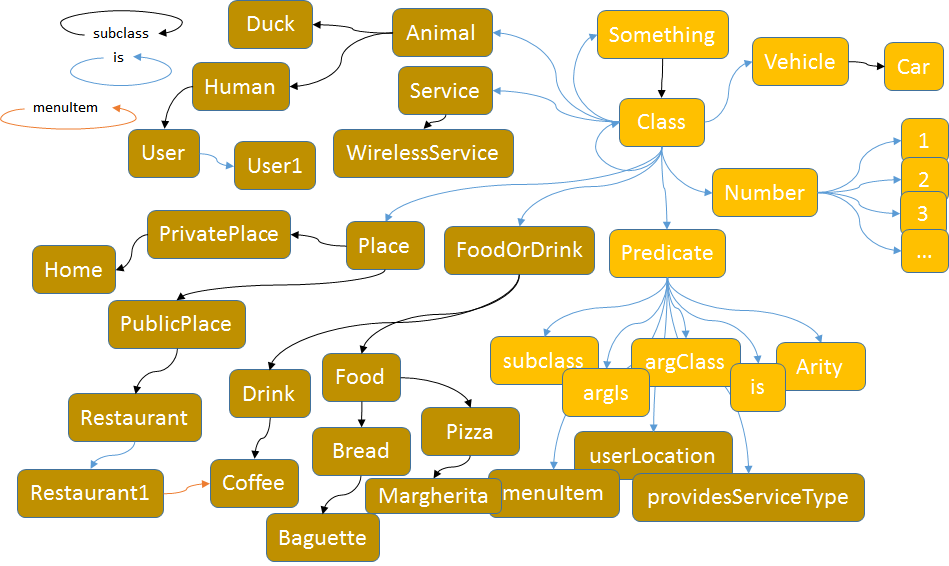
\includegraphics[width=1\textwidth]{figures/fullExistingKB.png}
	\caption{Current "existing knowledge" on top of upper ontology}
	\label{fig:existingKB}
\end{figure}

At tjhis point we have a formal KB structure representing a minimal 
\emph{existing knowledge} required to explan the examples from 
\autoref{tab:conversation1} and \autoref{tab:conversation2}. The KB is
graphically presented on the \autoref{fig:existingKB}, where the upper ontology
is presented in lighter color and new KB parts in darker. Due to lack of space,
the only relations are of $is$ (represented by blue arrows) and $subclass$ 
(represented with black arrows) predicates.

%SUBSECTION
\subsection{KA Knowledge}
\label{section:kakb}
In the previous two sections we defined the upper ontology
(Section \ref{section:upperOnto}) and then using its vocabulary to define the 
pre-existing knowledge (Section \ref{section:existingKB}). This will suffice to
support the explanation of the proposed KA approach. Similar as with the other
parts of the KB, listing full set of 
\emph{Curious Cat} KA rules would not fit in the paper. Instead we define an 
example set of the KB, sufficient for describing the approach and keeping the 
explanation as simple as possible. 

As a starting point, we need to define a main KA meta-class $Formula$, which’s 
is a special class (like $Number$).
\begin{definition}[class $Formula$ and its instances]\label{def:formula}
All logical formulas (assertions, queries) are instances of the class $Formula$.
Formally, this can be represented as:
\begin{equation}\label{as:formulas}
\begin{gathered}
	\forall P\forall x_{1...n}:is(P(x_1,...,x_n),Formula)
\end{gathered}
\end{equation}
Basically all of the content of the KB and queries are instances of $Formula$.
For example,assertion $userLocation(User1,Ljubljana)$ is an instance of 
$Formula$ and consequentially the statement
\begin{equation*}
is(userLocation(User1,Ljubljana),Formula)
\end{equation*}
is true.
\end{definition}
or simplicity we will be referring to the using string (") operator. 
For example: 

\subsection{Context}
\begin{definition}[predicate "$probableUserLocation$"]
\label{pred:probableUserLocation}
Dada\hl{Maybe define this one at the end, since it could also be defined in the
Context section}
\end{definition}

%
%------------------------------------------------------------------------------
% 
\chapter{Real World Knowledge Acquisition Implementation}
\label{chapter:implementation}
%-------------------------------------------------------------------------------
This chapter presents the actual implementation in the system described
in the previous chapters (especially in \autoref{chapter:approach}). While up 
to now we've been describing the idea and a general approach to do it 
(independent of the implementation), here we represent the actuall working
system that we implemented and kept it online in the shape of the current 
version since the end of 2012. 

\begin{figure}[H]
	\centering
		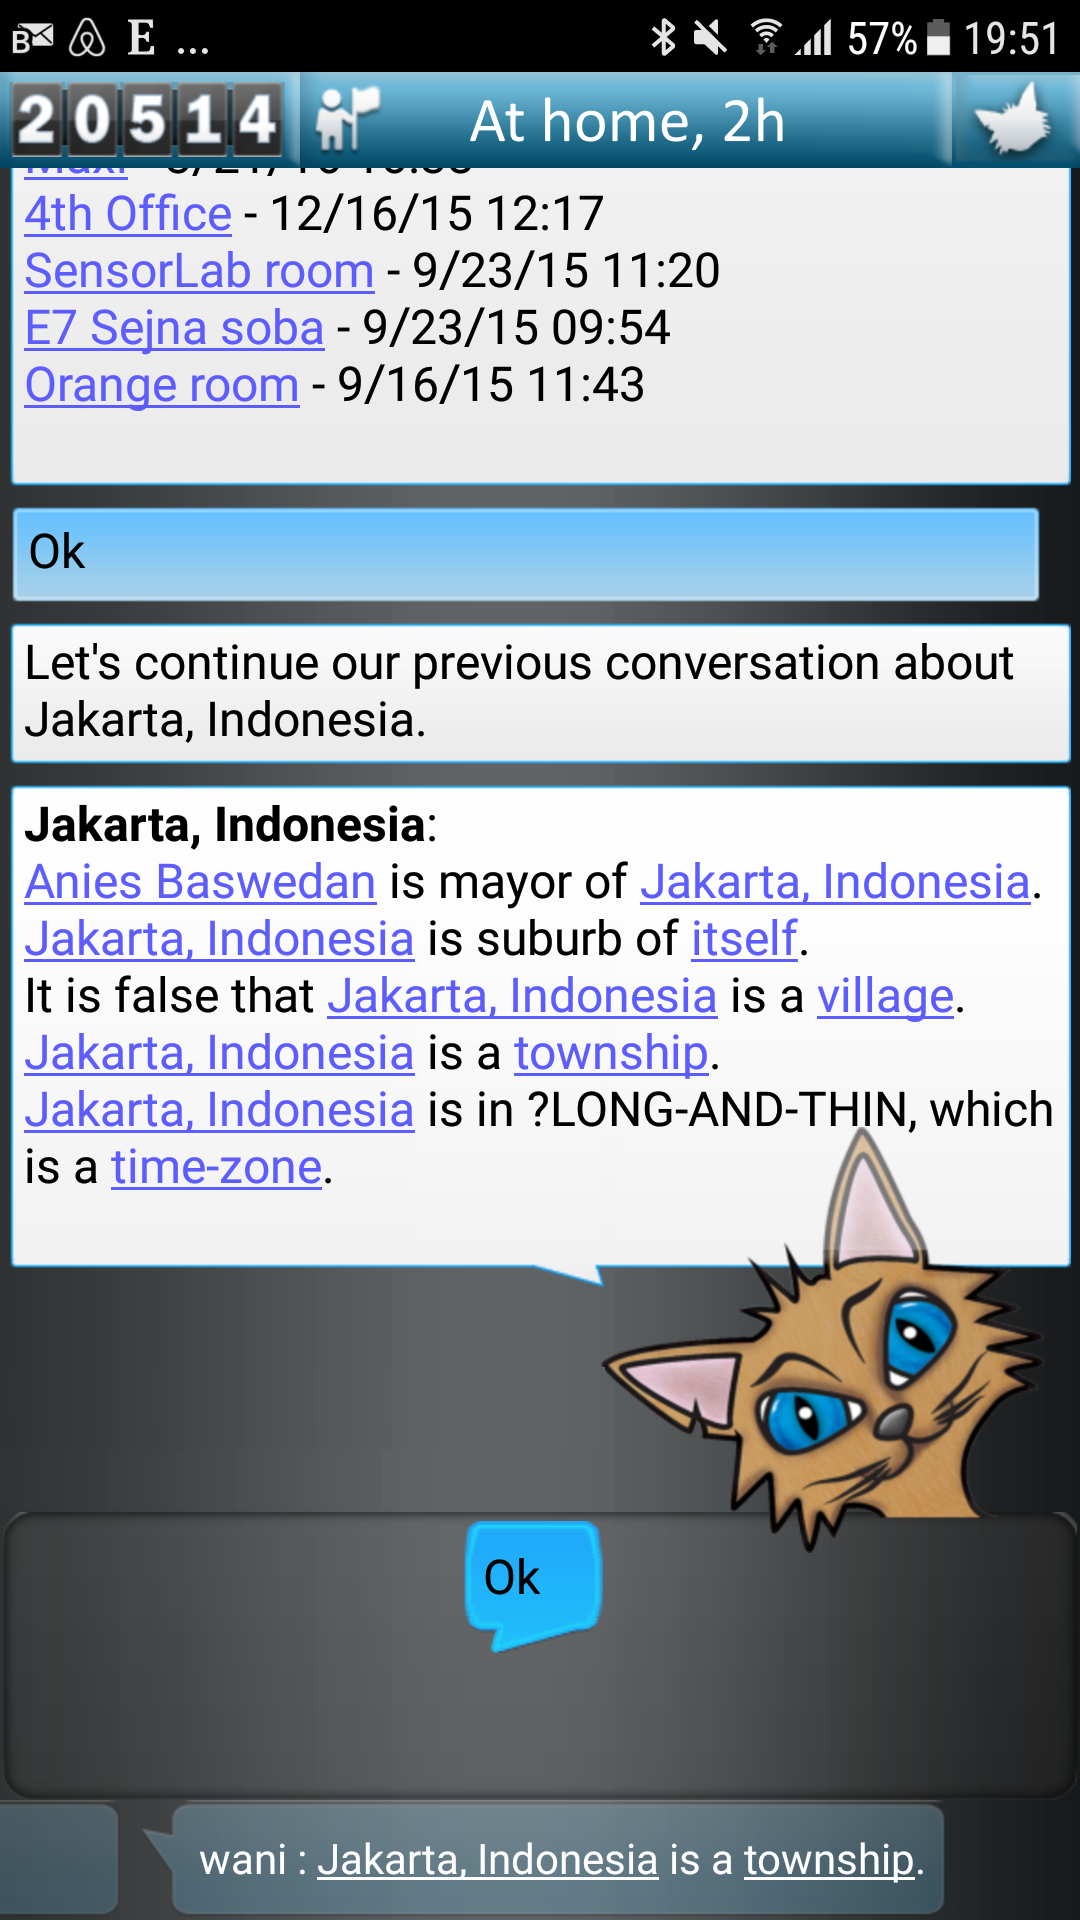
\includegraphics[width=0.41\textwidth]{figures/androidExample1.png}
	\caption{Screenshot of Curious Cat Android app.}
	\label{fig:androidExample}
\end{figure}

During this time, 5,185 users installed its
client app, out of which 2,401 users registered, and 1,715 users used it at 
least once (see the results chapter, \autoref{section:stickiness} for more 
details on users).
The development  of \emph{Curious Cat} implementation started on October 
26th, 2010 and halted on June 2014. The
implementation follows closely the architecture presented on 
\autoref{fig:Architecture} in \autoref{chapter:approach}. For the core
of the system we took Cyc with its common sense KB and inference engine, which 
was also an initial inspiration for the development and the approach, where
the main work needed to be done on the part of the meta-KB and also common
sense KB extensions to support our use-cases. For the NL modules, our 
implementation relies on the internal Cyc logic to NL conversion modules, and
on SCG\parencite{Schneider2015}. The procedural component and client were 
written from scratch. All together our implemented system consists of 50,686
lines of Java source code, and 12,616 lines of knowledge definitions (8,571) for
the additional knowledge we added in CycKB to drive our KA process.

Besides the implementation described here, this system was also implemented and
deployed as a real-time commuting companion\parencite{Figueiras2013}, and as an
RDF framework for on the field sensor information knowledge acquisition
\parencite{Bradesko2012a}. Commuting companion implementation and this implementation
were also described in the books \emph{Intelligent Decision Technology 
Support in Practice}\parencite{Costa2016} and \emph{Handbook of Human 
Computation}\parencite{Witbrock2013}. This implementation was also mentioned
in the \emph{Communications of the ACM} magazine article\parencite{Geller2016}.

Implementation consists of Android based mobile client (see screenshot on
\autoref{fig:androidExample}), Java Servlet based
\emph{Procedural Component} with PostGreSQL database access, two Research 
Cyc instances 
(KB, Inference Engine, NL Conversion) to increase the speed and reliablility 
of the system, \emph{Transcript Server} for syncing between Cyc instances, 
and a web-site for registration and email confirmation. This organization is 
also depicted on \autoref{fig:implementation} below.

\begin{figure}[H]
	\centering
		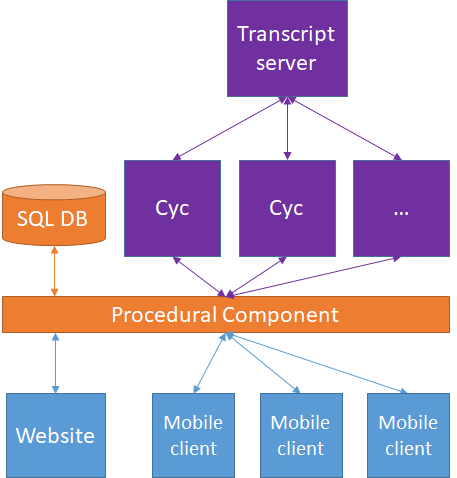
\includegraphics[width=0.62\textwidth]{figures/implementationOrg.png}
	\caption{Organization of the system modules in our implementation.}
	\label{fig:implementation}
\end{figure}

\section{Cyc}
\label{section:Cyc}
As already mentioned in related work (\autoref{section:relatedCyc}), \emph{Cyc}
is an AI project started in 1984 by Douglas Lenat\parencite{Lenat1985} with the
premise, that in order to make computers think like humans do, we need to first
make sure that they have same common sense knowledge as humans do. Since then,
\emph {Cyc} team (now part of \emph{Cycorp Inc.}), is codifying and entering 
the knowledge by hand and also by other means of knowledge acquisition and 
mining (see rows stating "Cyc" as parent in \autoref{tab:related}, 
\autoref{chapter:related} - \nameref{chapter:related}). 
The collected and codified knowledge is represented in machine-usable form 
using emph{CycL (Cyc Language)}, and is structured and grouped together as
\emph{CycKB}. In parallel with the KB, Cyc also contains an inference engine
that works on the scale of the KB, and a set of tools, APIs and other interfaces
for interacting with the system, ranging from web interface, natural language,
web APIs and also Java interfaces, which we used in our implementation and
communication with the procedural part of our system 
(\autoref{section:prophet}).

%subsection
\subsection{Cyc KB}
\label{section:cyckb}
At this moment (end of 2017), \emph{Research CycKB} consists of more than 
630,000 concepts, 7,000,000 assertions (rules are also assertions), made with
using more than 38,000 predicates (relations), covering a broad domain of
human common sense knowledge. The KB is divided into thousands of microtheories
(not counting the microtheories we added for \emph{CC} implementation - 
\autoref{section:crowdsourcing}), where each microtheory is a set of assertions
that share common assumptions. Microtheories (Mts) can hierarchically stack on 
top of each other and allow \emph{Cyc} to independently maintain assertions that
could contradict each-other. This also enhances the performance of the 
\emph{Cyc} inference engine, since it can be limited on one particular, or a
group of Mts to limit the number of facts it needs to use while inferencing.

\emph{CycKB} is represented in \emph{CycL}, with most basic syntax described as:
\begin{itemize}
\item Logical constants are represented by "$\#\$$" sign, followed by the name 
of the term name ($\#\$JoesPizza$).
\item Formulas are enclosed in parentesis. If more than one constants or terms
are part of the assertion, the predicate is always first, followed by its
arguments, for example: $(\#\$menuItem\quad\#\$JoesPizza\quad\#\$Pizza)$
\item Variables are represented by the question mark ("$?$") sign, followed
by the name in capital ($?PERSON$). For example, query asking the inference
engine, what is on the menu in Joe's Pizza is represented as: 
$(\#\$menuItem\quad\#\$JoesPizza\quad?ITEMS)$, where the name of the variable
"ITEMS", can be arbitrary.
\item Rules in \emph{CycKB} are represented by assertions using predicate 
$\#\$implies$, where the first argument is then it's antecedent and the second
argument a consequent (see CycL rule \ref{as:cycrule} below, which represents
the same upper ontology rule as defined in \hl{rule 4.10}).
\end{itemize}

Similar as with our example KB explaining CC approach, \emph{CycKB} is built on
top of upper ontology which gives it a formal grounding to support the rest of 
the KB. Our KA approach (\emph{Curious Cat} system) was implemented using 
\emph{Cyc}, and also inspired by its toolset and unsolved problems. CC 
initially started as a solution for Cyc to speed up the NL based KA, so for our
explanations it was natural to pick and define an \emph{Upper Ontology} that 
can be easily mapped to \emph{CycKB}. While we cannot directly map all of the
definitions we used to explain the approach, we can map most of the Upper 
Ontology, which is given in the table below.

\begin{table}[h]
\centering
\caption{Mapping between upper ontologies of Cyc and our example KB constructed
to explain the approach.}
\label{tab:uppermap}
\begin{tabular}{|l|l|}
	\hline
	\textbf{CC Upper Concept} & \textbf{CycKB Upper Concept}\\
    \hline
    $is$ & $\#\$isa$ \\
    \hline
	$subclass$ & $\#\$genls$ \\
	\hline
	$arity$ & $\#\$arity$ \\
	\hline
	$argIs$ & $\#\$argIsa$ \\
	\hline
	$argClass$ & $\#\$argGenl$ \\
	\hline
	$Class$ & $\#\$Collection$ \\
	\hline
	$Predicate$ & $\#\$Predicate$ \\
	\hline
	$Something$ & $\#\$Thing$ \\
	\hline
	$Number$ & $\#\$NonNegativeInteger$\\
	\hline
\end{tabular}
\end{table}

Similarly as with constants, some rules can be mapped into Cyc versions by 
replacing implication form ($x \implies y$), with the CycL form 
($(\#\$implies\quad (x) \quad (y))$. For example, rule \hl{4.10} is in
 \emph{CycL} written as follows:
\begin{equation}\label{as:cycrule}
\begin{gathered}
\begin{aligned}
&(\#\$implies\\
	&\quad(\#\$and\\
		&\qquad(\#\$genls\quad?X\quad?Y)\\
		&\qquad(\#\$genls\quad?Y\quad?Z))\\
	&\quad(\#\$genls\quad?X\quad?Z))
\end{aligned}
\end{gathered}
\end{equation}

%subsubsection
\subsubsection{CC KB}
\label{section:cckb}
Even though \emph{CycKB} is one of the biggest and most complete common sense 
KBs that currently exist, it still does not cover everything and has missing 
knowledge. While it covers at least a bit of almost any topic within the general
knowledge, it often has missing parts that need to be extended in order to use
the knowledge in real world. While this is exactly what \emph{Curious Cat} is
helping to solve, we also added some of the knowledge by hand, to make initial
questions more interesting and to make it cover more topics. For the whole CC
implementation, we added an additional 8,571 assertions on top of the existing 
7mio assertions of \emph{CycKB} prior knowledge.
\begin{itemize}
\item New assertions are mostly KA meta-knowledge supporting the acquisition
mechanisms and logic.
\item Some of the new assertions are also missing general knowledge 
improvements on top of CycKB.
\end{itemize}

For the initial \emph{Cyc} knowledge entry process, we used ".ke" files, 
which support bulk import bigger amount of the assertions (see 
\autoref{fig:ketext}). After the system was already stable and running all the
time, this was replaced by the Transcript Server syncing as described below
in \autoref{section:transcriptserver}.

\begin{figure}[H]
	\centering
		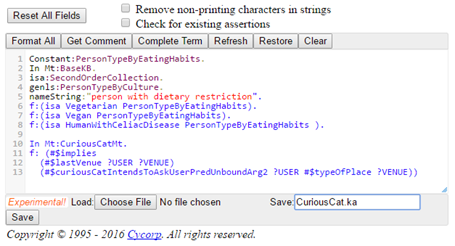
\includegraphics[width=0.9\textwidth]{figures/keEntry.png}
	\caption{Example screen of bulk importing assertions (knowledge) into Cyc.
This example is defining a concept $PersonTypeByEatingHabits$ and a rule 
generating questions about typeOfPlace for last known user venue visit.}
	\label{fig:ketext}
\end{figure}

While mapping from our explanations to the actual \emph{Cyc} upper ontology is 
pretty straight forward since it is small, it would be impossible to describe
all details of more than 8,000 assertions that define the implementation of
CC KA approach. For example, the simple $ccWantsToAsk$ predicate (see
\hl{definition 4.15 in chapter X}, alternative in the real-world implementation
is 8 predicates (see definition \ref{as:cycCCAssertions} below), allowing us to define much more complicated statements and
enriching them with possible suggestions as visible on \autoref{fig:ccmediated}.
Similary, the KA rules are more complicated, using much bigger vocabulary
than we were able to exaplain. Example of one such rule is presented on
\autoref{fig:kaRuleImpl}.

On top of 7 million of pre-existing \emph{Cyc} assertions and 8,571 of manually
added CC assertions, our system collected from users additional 524,276 
assertions (as of September 2017).

\begin{figure}[h]
	\centering
		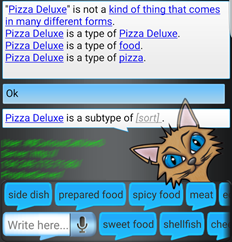
\includegraphics[width=0.4\textwidth]{figures/androidMediated.png}
	\caption{Example of human to computer interaction options generated with
$\#\$curiousCatIntendsToAskUserPredUnboundArg2WithChoices$.}
	\label{fig:ccmediated}
\end{figure}

\begin{figure}[h]
	\centering
		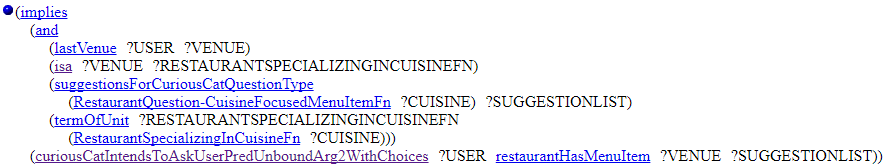
\includegraphics[width=1\textwidth]{figures/kaRule.png}
	\caption{Example of KA rule from CC implementation (screenshot from Cyc).}
	\label{fig:kaRuleImpl}
\end{figure}

\begin{equation}\label{as:cycCCAssertions}
\begin{gathered}
\begin{aligned}
&S_{CC Intents}=\{\\
&\quad\#\$curiousCatIntendsToAskUserPredBound,\\
&\quad\#\$curiousCatIntendsToAskUserPredUnboundArg2,\\
&\quad\#\$curiousCatIntendsToAskUserPredUnboundArg2WithChoices,\\
&\quad\#\$curiousCatIntendsToAskUserPredUnboundArg3WithChoices,\\
&\quad\#\$curiousCatIntendsToAskUserYesNoQuestionAboutVenue,\\
&\quad\#\$curiousCatIntendsToAskUserYesNoQuestionAboutVenueWithArgument,\\
&\quad\#\$curiousCatIntendsToAskWithChoices,\\
&\quad\#\$curiousCatWantsToAskUser\\
&\}
\end{aligned}
\end{gathered}
\end{equation}

%subsection
\subsection{Cyc Inferene Engine}
\label{section:cycinference}
Cyc AI system also includes the inference engine which can work over the CycKB.
Because the KB is so big (more than 7 million assertions), approaches taken
by other inference engines (like RETE algorithm) does not scale well at this
size, while the included engine is with some tweaking still able to give 
results inside tolerable time frame. One of the techniquies (mentioned before)
allowing this, is organization of the KB into microtheories which allow the 
inference engine to reduce the size of the world it operates with at given
contexts.

Cyc Inference Engine is able to perform modus ponens and modus tollens 
inference, universal and existential quantification, and also mathematical 
calculations\footnote{http://www.cyc.com/subl-information/introduction-cyc-inferencing/overview-cyc-inferencing/}. The inference engine is constructed together
with a set of \emph{Inference Removal Modules} (each module is able to remove or
solve a specific problem from the inference problem). These modules can range
from very general, to very specific ones, registered to only solve problems
related to one particular logical predicate. For example, predicate 
$\#\$disjointWith$ can have a module that can tell whether the assertions using
this predicate are true or not (decides on disjointness). There are many
modules like this, implementing symmetry, transitivity and reflexivity, etc.

The engine is mostly controlled with rules (as are rules \hl{some rules} and
the KA rule on \autoref{fig:kaRuleImpl}). The inference rules can be separated
into the forward and backward rules, which define whether they are to be used
by forward chaining or backward chaining while doing the inference. Forward
rules are triggered when something is asserted into the KB and then they produce
the results (assertions as defined in the consequent), while backward rules
are triggered when a logical query is being asked over the KB, and only support
the logic behind the answering, without actually physically populating the KB.
The example KA rule from the \autoref{fig:kaRuleImpl} is forward rule. 

Forward rules are causing the system to be slower when something is being added,
and also cause its memory consumption to increase (newly inferred assertions),
but on the other hand speed up the querying. Backward rules are the opposite,
not taking any burden on the system when the assertion is being added, but
trigger the inference which could be slow, when someone issues a query.

%subsection
\subsection{Cyc NL}
\label{section:cycnl}
In the \hl{section NL} and \hl{section NL2SCG} we gave a simplest possible 
example of logic to NL and the opposite conversion, to explain and showcase the
approach taken by the \emph{Curious Cat}. While this served well for the
explantion, the implementation in real-world is inherently more complicated.
For the implementation we used Cyc logic to NL system which is part of 
\emph{Research Cyc}\autocite{Coppock2010,Baxter2005}, and is able to convert
a decent number of \emph{CycL} assertions into thier natural language 
equivalents. In our example, we only used two (2) predicates to be able to
do that ($name$, $nlPattern$), but the implemented system uses more than
90 predicates and functions that are used to make the paraphrase system to work.
On the \autoref{fig:nlAssertion}, we can see the screenshot of
NL generation assertion using 4 paraphrase functions, unbound variables,
a string and a concept of the $Have-TheWord$. Then additionally, the concept
representing the word "have", has additional 79 language generation assertions
defining how to convert this word in various discourse contexts. 

\begin{figure}[h]
	\centering
		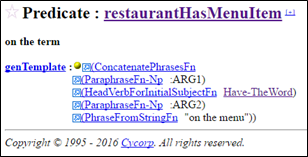
\includegraphics[width=0.6\textwidth]{figures/nlAssertion.png}
	\caption{Actual NL generation assertion example for the corresponding predicate for 'menuItem' from our implementation (Cyc).}
	\label{fig:nlAssertion}
\end{figure}

As part of implementing \emph{CC}, we had
to extend this sytem and add multiple NL generating assertions to it, the
implementation is from \emph{Cyc AI System}, and is out of scope of this 
thesis. The details of this approach which can generate both referring 
expressions and non-referring expressions, including both referential and 
bound variable anaphora, are described in the paper written by
\textcite{Coppock2010}. 

To be able to convert from NL back to logic, our implementation also relies on
the functionality which is part of \emph{Cyc} and is described in more detail
in the Semantic Construvtion Grammar paper\parencite{Schneider2015}. The 
approach is similar as
taken by chat-bot engines\parencite{Wilcox2011}, which uses textual patterns
with special wildcards, to map the actual text onto a pre-defined pattern, which
is then used to find a response. The difference is, that after the initial 
pattern matches are found, it uses \emph{CycL} mappings and then Inference 
Engine to check for
the formal validity of the resulting statements and consequently the parsing 
process. The other improvement is, that the the wildcards in the patterns
can be typed (using Cyc constants). This means that that in such patterns, 
only terms of specific type can be fitted into a slot, which improves the 
conversion accuracy. An example pattern (taken from the paper) can be written 
like: "place[d|\{\}] \$ContainerArtifact\#0 over high heat".
During the years of CC experiment (as described in the 
\autoref{section:evaluation}), the logic to NL was used all the time (it is a
crucial component), while NL to logic was implemented but not always used, 
because it is more complex part of the software, harder to maintain, and was
also not of crucial importance for KA experiments.

%subsection
\section{Transcript Server}
\label{section:transcriptserver}
The \emph{Transcript Server} is an important technical part of the presented CC 
implementation, improving scalability, reducing downtime and also reducing
other maintenance costs. As visible in the implementation design 
(\autoref{fig:implementation}) sketch, it is a clowd based software module
to which all Cyc instances connect to. Software wise it is a simple database
server, which can receive and store for later, raw \emph{CycL} assertions 
(without any inference capabilities), and replicate them between 
connected \emph{Cyc} instances. Each of CC instances of \emph{Cyc} system is
set in a way, that after it wakes up, first syncs with the \emph{Transcript 
Server} and thus gets the knowledge added in the past. Besides the syncing,
it also forwards every new assertion to the \emph{Transcript Server} (if it was
not received from there). 

This simple mechanism allows us to have multiple \emph{Cyc} instances with
the same knowledge, which then allows simple load-balancing at query-time,
backup instances in cases when the main instance crashes. For the cases when
we had to manually shut down Cyc for upgrades or server maintenance, this simple
automatic syncing mechanism (even if being slow due to each assertion triggering
the inference engine again), saved us a lot of manual importing of the old knowledge. As of September 2017, full sync of CC collected knowledge (532,847 
assertions) takes approximately 2 days to finish.

%section
\section{Mobile Client}
\label{section:app}
The client part of the implemented KA approach is a simple Android application
(see screenshot on \autoref{fig:androidExample} at the beginning of the chapter).
The main screen consists of (listed top down as sections appear on the phone 
screen):
\begin{itemize}
\item Upper status bar, containing the points on the left, location info and 
button in the middle, ant a "cat" menu on the right.
\item Middle conversational section, where CC and user responses appear as
text in the conversational bubbles, similar to those that usually represent 
SMS messages. Each bubble can contain html formatted text, hyperlinks and 
pictures.
\item Conversational section is followed by the "response section", where user
is presented with the set of possible responses, or a free text box. On the 
right of this GUI section, there is a cat's face, which acts as a button with
same functionalities as the "cat" menu on the upper right.
\item On the bottom, there is a swipable section, which contains contextual
bubbles representing what other users  who are nearby or are discussing same 
topics are answering.
\end{itemize} 

The logic behind the client is pretty straight forward. It is connected to the
\emph{Procedural Component} of CC system, which can send it a discourse object
containing a text which needs to be presented to the user, and some additional 
info such as ID of the statement, it's \emph{CycL} representation and also
suggestions for the user, and the points that user currently collected. When 
the user answers, this is sent back to the server, together with the ID of the 
discourse. In the cases, when the server wants to pro-actively ask something,
and the phone is in a sleep mode (meaning that the proactivity didn't occur due
to location change), it can generate a FCM message with the same object as
it would send directly, and then this is presented to the user when he/she 
looks at the phone.

Additionally to this answer/reply functionality, represented as blue arrows on
\autoref{fig:Architecture}, the client keeps a back-channel with the 
server's \emph{Procedural Component}, and is periodically sending a location,
local time and language. In order to not consume a lot of the battery, the 
client is mostly sleeping, and only wakes up every 3min and tries to get a GPS
signal for 20 seconds. If the signal is too low and cannot acquire accurate 
enough location in 20 seconds, it stops trying and goes back to sleep mode.
The back-channel is also opened each time user opens the client application
manually.

%section
\section{Procedutal Component}
\label{section:prophet}
d


% 
%--------------------------------------------------------------------------------
% 
\chapter{Evaluation}
\label{chapter:evaluation}
%--------------------------------------------------------------------------------

Validation of the proposed approach was performed using our \emph{Curious Cat}
implementation of the proposed KA approach, running alive over the course of 4 
years engaging a total of 728 registered 
users (users which are part of the experiment. Overall the implementation have
some additional users). During that time, the users checked-into 5,551 locations
and responded 
to 57,978 questions, out of which 8,611 were voting questions (7,560 positive 
and 1,051 negative votes), 18,907 questions were answered with "I dont know", 
and 30,460 real answers was inserted into the KB as new knowledge, including 
31,140 concepts (3,171 connected to instances of $User$ concept, 22,563 
check-ins and other places, and 5,406 other concepts). 
These triggered additional 386,980 assertions to be added through 
forward-chained inference. These can be separated into facts (374,300 
assertions) and additional derived question generating rules and questions 
(12,680). Altogether we gathered \textbf{444,958 (374,300 + 30,460)} pieces of 
completely new knowledge. 

For easier understanding of the results, we show the structure of the collected
knowledge 
graphically in \autoref{fig:results}, and give real examples of the collected 
and inferred knowledge in \autoref{tab:ccresultexamples}.

\begin{figure}[h]
	\centering
		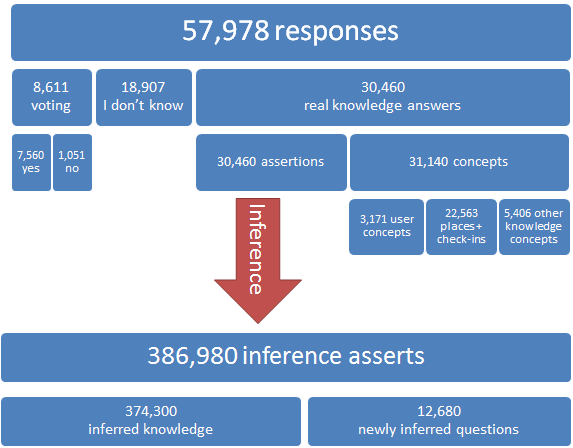
\includegraphics[width=1\textwidth]{figures/results.png}
	\caption{Graphical representation of collected answers (knowledge) and 
    distributions.}
	\label{fig:results}
\end{figure}

\begin{table}[h]
\centering
\caption{Examples of answered/asserted and inferred knowledge taken from
\emph{Curious Cat} KB.}
\label{tab:ccresultexamples}
\begin{tabular}{|c|l|l|}
	\hline
	\makecell[l]{\textbf{Type of the} \\ \textbf{collected knowledge}} & \textbf{Curious Cat Question} & \textbf{User Answer} \\
    \hline
    \textbf{User Concepts} &\makecell[l]{[automatic assert \\from registration]} & \makecell[l]{$is(User1,Person)$, \\ $name(User1,"Luka")$} \\
    \hline
    \textbf{Places + Check-ins} &\makecell[l]{[automatic assert \\from check-in \\ and Foursquare/\\Factual locations]} & \makecell[l]{$is(Place1,Restaurant)$, \\ $name(Place1,$\\"Pig'n Whistle"$)$} \\
     \hline
    \textbf{Other Concepts} &\makecell[l]{What did you order?} & \makecell[l]{Duck meat} \\
	\hline 
    \textbf{Real Knowledge 1} & Who is CEO of BMW? & Harald Kruger\\
	\hline
    \textbf{Real Knowledge 2} &\makecell[l]{What is the ticker symbol\\ of BMW?} & ABC \\
	\hline
    \textbf{voting(yes)} &\makecell[l]{Is it true that Herald Krueger\\ is the CEO of BMW company?} & yes \\
	\hline
    \textbf{voting(no)} &\makecell[l]{Is it true that ABC \\is the ticker symbol for BMW?} & no \\
	\hline
    \textbf{I don't know} &\makecell[l]{\_\_\_ and BMW are \\corporate competitors.} & I don't know \\
	\hline
    \textbf{Inferred knowledge 1} &\multicolumn{2}{l|}{$is(HeraldKrueger,Person)$} \\
	\hline
    \textbf{Inferred knowledge 2} &\multicolumn{2}{l|}{$anatomicalParts(HeraldKrueger,Hand)$} \\
	\hline
    \makecell[l]{\bfseries{Newly Inferred}\\ \bfseries{question}} &\multicolumn{2}{l|}{"What is Herald Krueger's age?"} \\
	\hline
\end{tabular}
\end{table}

While the resulting number and quality (\autoref{tab:baselines}, 
\autoref{tab:validity}) of assertions
shows that the presented approach can be successfully used for high quality KA,
we explored in more detail the contributions of specific characteristics of our
system and compare them to the baselines, to evaluate the ideas and claims
of the approach:
\begin{enumerate}
\item Using context to proactively drive the KA increases engagement and the 
chance of getting an answer (\autoref{section:evaluationContext})
\item Pre-existing knowledge and automated inference can be used to filter-out 
inconsistent answers and thus increase the quality of the acquired knowledge
\item Using newly acquired knowledge to further drive the KA process increases
the amount of acquired answers and reach of the system
\item Crowdsourcing additionally improves the results by filtering wrong but 
logically correct answers
\end{enumerate}

\section{Context and Proactivity}
\label{section:evaluationContext}
\emph{Curious Cat} employs two contextual knowledge provision mechanisms. One 
is location based knowledge, such as, the type of current location, the time of
visit and the duration of stay. The second is internal knowledge that the 
system already knows about the user, such us, languages that the user speaks, 
food she likes, demographics data, interests, etc. In evaluation, we focused on
exploring benefits of using the location based context, since it is practically
impossible to disable internal knowledge without bigger changes in the system. 
Inferring without internal knowledge e.g., total removal of the personal 
knowledge would mean removal of almost all questions regarding people, animals,
human interests, etc., since these are general for human beings and to some 
extent to animals as well.

For the purpose of this experiment, we deliberately removed GPS location and 
connected mechanisms for derived knowledge for a duration of three months. We 
normalized the measures (assertions per user per day) for all experiments to 
level out the differences in the durations of experiments against a longer 
duration of fully operative system. The results are presented in 
\autoref{tab:ccresultscompare}. The columns in the table are organized as 
follows:

\begin{itemize}
\item first column contains measure name,
\item second column full data-set when using context (marked as C),
\item third is 100-day data-set when not using context (NC100),
\item and last is the normalized column with context (C100) which makes it 
possible to compare the context versus no context knowledge collection behavior (C100 vs NC100).
\end{itemize}

Since number of days and users is strongly correlated with the number of 
answers the system gets, and we only have the "No Context" data for 100 days 
(41 new users during that time and 45 active users), we normalized our 
"Context data" in such a way, that it matches the duration, new users and 
active users of \emph{NC100}. For this, we had to scan all the data-set 
day-by day with a range of 100-day window, where we looked at the number of new 
and active users in each of the 1264 sub-windows (number of all different 
100 day windows one can fit into 1264 days). In the whole data-set there was 
18 such 100-day windows, which can be directly compared to the \emph{NC100}. 
While the number of new users is fixed to 41, number of new assertions and 
active users still varies (min. 1,429, max. 9,279 new assertions and min. 47, 
max 61 active users). For this reason, we calculated the mean values of all 
18 windows which had the same number of new users as \emph{NC100}. Matching 
new users (instead of active users) was selected because new users are the
ones that contribute most of the assertions, since their interest winds down 
gradually. This can be seen on \autoref{fig:followups}. This is also the 
primary reason why (unintuitively) number of new assertions/day/active user 
(row 7 in {utoref{tab:ccresultscompare}) is higher without context 
(\emph{NC100}) than for  non-normalized data from experiment using context 
(\emph{C}).

\begin{table}[h]
\centering
\caption{Results of KA without context versus results while using location based context}
\label{tab:ccresultscompare}
\begin{tabular}{|l|l|l|l|}
	\hline
	\textbf{Measure}  & \makecell[l]{\textbf{With Location}\\\textbf{Context (C)}} & \makecell[l]{\textbf{Without Location}\\ \textbf{Context (NC100)}} &  \makecell[l]{\textbf{With Location}\\\textbf{Context 100}\\\textbf{days (C100)}}\\
    \hline
    1. Experiment duration & 1,364 days & 100 days & 100 days \\
    \hline
    2. Number of new assertions & 56,586 & 709 & 2,244 (+216.5\%) \\
    \hline
    \makecell[l]{3. Number of new assertions\\where user didn't\\ know the answer} & 18,380 (32\%) & 267 (38\%) & 667 (28.3\% = -9.7\%) \\
	\hline 
    \makecell[l]{4. Number of new \\assertions where \\user knew the answer}  &38,206 (68\%) & 442 (62\%) & 1,577 (71.7\% = +9.7\%) \\
	\hline
    \makecell[l]{5. Number of new \\assertions/day \\(all users) } & 42.1 & 7.1 & 22.4 (+215.5\%)\\
	\hline
    \makecell[l]{6. Number of new \\assertions/active user } & 90.3 & 15.7 & 44.2 (+181.5\%) \\
	\hline
    \makecell[l]{\textbf{7. Number of new}\\\textbf{assertions/day/active}\\\textbf{user}} & 0.07 & 0.16 & \textbf{0.44 (+175\%)} \\
	\hline
    \makecell[l]{8. Number of new \\concepts/day} & 3.7 & 0.4 & 2.4 (+85.2\%) \\
	\hline
    \makecell[l]{9. Number of new concepts \\ (excluding users and\\ locations)} & 4,925 & 36 & 243 (+85.2\%) \\
	\hline
    10. Number of active users & 625 & 45 & 49 \\
	\hline
    11. Number of new users & 625 & 41 & 41 \\
	\hline
\end{tabular}
\end{table}

The results of not using context show the decrease of raw new knowledge 
assertions from 56,568 to 709, which of course can be attributed to the fact 
that duration of experiment \emph{C} was much longer, or that it had more users
than \emph{NC100}. As described above, this is properly normalized in the 
column \emph{C100}, where the raw number of assertions raises to 2,244 
compared to only 709 when not using context (\textbf{context brings 217\% 
increase}).

While the majority of the increase is due to pro-active questions from 
\emph{Curious Cat}, which are linked to GPS clustering, some of the increase 
is also due to better targeting of the questions due to contextual data, 
since without the context only users are selecting the topics and the system 
doesnt have enough knowledge to successfully pick the most relevant next 
question. This is reflected in a slight increase in the proportion of the 
questions for which the user knows the answer (+9.7\% - row 4 in 
\autoref{tab:ccresultscompare}). This is independently of pro-active component 
which is mostly reflected in the raw number of assertions, while the 
knowing/not knowing ratio improvement is due to better targeting whatever 
question there was.

%subsection
\subsection{Consistency Checking}
\label{section:resultsConsistencyChecking}
Before the system accepts the answer from the user (as described in 
\autoref{section:consistency}), it converts it into logic and checks whether it 
is consistent with its current knowledge. If there is an inconsistency, it will 
reject the answer and thus prevent the wrong or contradicting knowledge to 
corrupt the KB and consequently the future KA process. The user then either has
to fix the answer, or convince the system that the answer is actually only a 
different name for the consistent knowledge. For example, if the user states 
that he ate a car in the restaurant, this is either wrong, or car is the name 
for some unknown food and not a vehicle.

Due to development process and timeline of the system, we only have logs and 
consequently insights on when/how the system rejected the answers due to 
inconsistency for 143 out of 1,472 days of the experiment duration. During 
this time, 148 users provided 23,543 answers and the system rejected 563 of 
them, so 22,980 of assertions went into the KB. Among the 563 rejections, 
some of them were repeating (user re-tries, or other users did the same 
mistake), so the system actually prevented 384 unique inconsistent answers.

%old table VII
\begin{table}[h]
\centering
\caption{Results of Consistency Checking}
\label{tab:resultsconsistencycheck}
\begin{tabular}{|l||l|l|}
	\hline
	\textbf{Measure}  &	 \makecell[l]{\textbf{Real data from}\\\textbf{the logs}} & \makecell[l]{\textbf{Extrapolation for}\\ \textbf{the full experiment}} \\
    \hline
    Number of new assertions & 22,980 & 57,978 days \\
    \hline
    \makecell[l]{Number of rejected assertions\\due to inconsistency} & 563 & 1420\\
    \hline
    \makecell[l]{\textbf{Percentage of rejected}\\\textbf{asserts}} & \textbf{2.45\%} & \textbf{2.45\%} \\	
	\hline 
    \makecell[l]{Number of unique rejected\\ asserts} & 384 & 968 \\
	\hline
    \makecell[l]{\textbf{Percentage of unique}\\ \textbf{rejected asserts}} & \textbf{1.67\%} & \textbf{1.67\%}\\
	\hline
    \makecell[l]{Number of new users } & 128 & 728 \\
	\hline
    \makecell[l]{Number of active users} & 148 & 728 \\
	\hline
    \makecell[l]{Experiment duration} & 143 days & 1472 days \\
	\hline
\end{tabular}
\end{table}

As presented in \autoref{tab:resultsconsistencycheck}, for every 100 valid 
answers users provided during the experiment, there were 2.45 answers which 
were rejected by the system due to being completely wrong or inconsistent. 
Because we only have logs for 143 days we had to extrapolate the number for the
overall experiment to get some estimation of how many bad assertions were 
prevented by the system throughout the whole experiment. The estimated number 
of rejected assertion system prevented overall is 1,420. Fore easier 
understanding, in \autoref{tab:rejectedconversation} are examples of the 
rejected assertions, together with the interaction that lead to the rejection.

%old table VIII
\begin{table}[h]
\centering
\caption{Conversation prior to rejected assertions}
\label{tab:rejectedconversation}
\begin{tabular}{|l|l|}
	\hline
	\textbf{CC}  & \textbf{User} \\
    \hline
    \multicolumn{2}{|c|}{\textbf{Example 1}} \\
    \hline
    \makecell[l]{Which social being has \\ Lagos as assets?} & hotel \\
    \hline
    \makecell[l]{By hotel do you mean\\ hotel (building)?} & yes\\
    \hline
    \multicolumn{2}{|l|}{\textbf{Rejected - building is not a social building}}\\
    \hline
    \multicolumn{2}{|c|}{\textbf{Example 2}} \\
    \hline
    \makecell[l]{Let's continue our\\ previous conversation \\ about going on a date.} & ok \\
    \hline
    \makecell[l]{All going on a date has\\ \_\_\_as a characteristic\\sub-event} & hello\\
    \hline
    \multicolumn{2}{|l|}{\textbf{Rejected - hello is a greeting, not an event.}}\\
    \hline
\end{tabular}
\end{table}

%subsection
\subsection{Additional knowledge as follow-up of newly acquired knowledge}
\label{section:followups}
As one of the more important features of our proposed system is its ability to 
use newly acquired knowledge to ask new things, we explored this functionality, 
comparing it to the baseline KA and consequently measuring the knowledge that 
was acquired as a consequence of prior acquisition. An example of such a 
follow up question or assertion is given in \autoref{tab:followupexample}.

%old table IX
\begin{table}[h]
\centering
\caption{Example of follow-up question and answers (new knowledge)}
\label{tab:followupexample}
\begin{tabular}{|c|l|}
	\hline
	1  & CC Asks: "What did you order?" \\
    \hline
    2 & User answers: "Meatloaf" \\
    \hline
    3 & \makecell[l]{CC asks a follow-up question: "One of the meatloaf\\ ingredients is \_\_\_". }\\
    \hline
    4 & User answers: "egg". \\
    \hline
\end{tabular}
\end{table}

The question number 3 in \autoref{tab:followupexample} is a "follow-up" question
since it is only asked when someone enters the previously unknown food concept. 
Answer under number 4 is a follow-up knowledge, since it was answered and given 
to the system only because someone created the concept of $Meatloaf$.

During the whole experiment the system collected and accepted \textbf{22,838 
answers}, which were a follow-up answer. This means that \textbf{39.4\%} of all
the knowledge we obtained was a direct consequence of the systems ability to 
generate new questions based on the already acquired knowledge.

The follow-up questions and answers are always a consequence of some new 
concept that enters the system. The 22,838 of answers are consequence of 
5,406 new concepts (not counting concepts of users themselves and locations 
they checked in), where the distribution of new knowledge/concept follows a 
long-tail distribution - a very small number of concepts triggered a big number
of follow-up knowledge (\autoref{fig:followups} - logarithmic scale).

\begin{figure}[H]
	\centering
		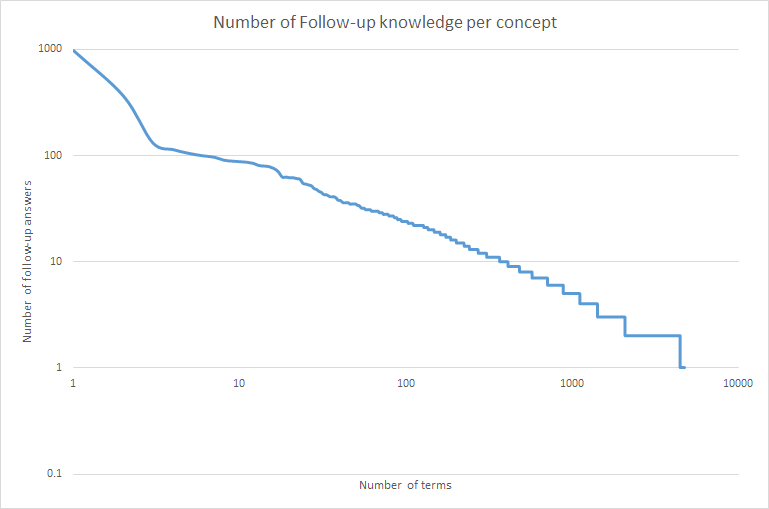
\includegraphics[width=1\textwidth]{figures/followupGraph.png}
	\caption{Long tail (logarithmic scale) distribution of follow-up answers per new concept}
	\label{fig:followups}
\end{figure}

%subsection
\subsection{Additional knowledge because of allowing cross-user cooperation}
\label{section:resultscross}
Similarly, as done for follow-up answers in \autoref{section:followups}, we can
check how much of the new knowledge came into the system due to its ability to 
share knowledge and questions cross-users. For this, we check the answers, 
where the initial concept was given to the system from a different user then the
follow up answer. From the example in \autoref{tab:followupexample} this would 
mean that the answer number 2 was given by $User1$ and then CC asks the 
question 3 and receives answer 4 from $User2$.

While for follow-up results, we have a complete log, due to changing the 
system, not all records have information about the original user who created 
the concept. We have his data only for 45 concepts out of 5406, excluding all 
user concepts and locations they checked-in. For these 45 concepts, 
we got additional 123 answers from other users.

%subsection
\subsection{Voting}
\label{section:resultsvoting}
The voting part of the system is, besides directly providing the answers, 
one of the main crowdsourcing components. As described in 
\autoref{section:crowdsourcing}, 
after the knowledge is acquired, the system can re-check with other users 
whether the assertion is true or not. This is done by presenting a question in 
the form: "Is it true that [assertion].", which can be answered with "yes" or 
"no". For example: "Is it true that Bornholmsk is a national language of 
Denmark?".

While the consistency check is performed automatically by the system, the 
answers that are manifestly inconsistent with the other content in the KB are 
stored only in the user specific part of the KB. Checking for truth of the 
knowledge is motivated by the fact that claims can be still be untrue even if 
they are consistent with the KB. From the Yes/No ratio, we can see that there 
are many more "Yes" votes than "No" votes, which hints that the answers the 
other users provide are mostly recognized as true by the crowd. 
This could be taken as a hint towards the precision of the truthfulness of the 
acquired knowledge. If we take into consideration that more users can vote for 
the same assertion, the effective precision of the knowledge measured this way 
can be estimated more accurately. The voting mechanism hides from the public 
knowledge base 97 of the assertions where the users were unable to agree on 
truth and 636 assertions which were voted as untrue by majority of the users.

%old table X
\begin{table}[h]
\centering
\caption{Crowd voting results}
\label{tab:votingresults}
\begin{tabular}{|l|l|}
	\hline
	\textbf{Measure}  & \textbf{Number} \\
    \hline
    All votes & 8,611 \\
    \hline
    Votes over unique asserts & 5,436 \\
    \hline
    Yes votes & 7,560 \\
    \hline
    No votes & 1,051 \\
    \hline
    Rejected answers & 636 \\
    \hline
    Accepted answers & 4,703 \\
    \hline
    Undecided answers & 97 \\
    \hline
\end{tabular}
\end{table}

If we look at some of the most rejected assertions, we can see assertions 
such as (more no votes than yes):
\begin{itemize}
\item $nationalLanguage (Denmark Bornholmsk)$ (3 yes, 9 no)
\item $typicalColorOfType (Automobile BlackColor)$ (3 yes, 9 no)
\item $is (CityOfCopenhagenDenmark Town)$ (0 yes, 4 no)
\item $subclass (Coffee-Beverage ArtificialMaterial)$ (3 yes, 9 no)
\item $soleMakerOfProductType (TelevisionSet PhilipsPetroleumCompany)$ (3 yes, 7 no)
\end{itemize}
And the most accepted assertions (more yes votes than no):
\begin{itemize}
\item $is (Denmark CountryWithOnlyOneTimeZone)$ (25 yes, 0 no)
\item $is (Food CollectionWithManySpecializzations)$ (23 yes, 0 no)
\item $sublcass (Food OrganicMaterial)$ (19 yes, 0 no)
\item $is (Food ProductTypeWithoutSoleMaker)$ (20 yes, 1 no)
\item $countryPhoneCode (Slovenia 386)$ (18 yes, 0 no)
\end{itemize}
And some of the undecided assertions (same number of yes and no votes):
\begin{itemize}
\item $subclass (IceCream Mixture)$ (2 yes, 2 no)
\item $characteristicProperSubeventTypes (CookingFood EatingEvent)$ (1 yes, 1 no)
\item $electronicDeviceMountingStyle (RearVideoPort DesktopComputer)$ (2 yes, 2 no)
\end{itemize}

%subsection
\subsection{User Stickiness Factor}
\label{section:stickiness}
To get an idea of how the users interacted with the system, we checked each of
them by the first and the last piece of knowledge they provided and measured 
the duration of days between these dates. This is a simple indicator of a 
stickiness - showing how many of the users only tried an application and then 
forgot about it and how many of them answered questions for longer. On
\autoref{fig:userstickiness} we can see the long-tail distribution of how long 
users stick with the application. About 25\% of the users stick with the 
system for more than just one-day testing. While most of the users (548) only 
tested the system for a day and did not use it further, 180 users stayed for a 
longer period of time. Among these, 117 used it for more than a week, 98 for 
more than two weeks, 69 for a month or more, 51 for more than two months and 
15 for more than a year.
\begin{figure}[H]
	\centering
		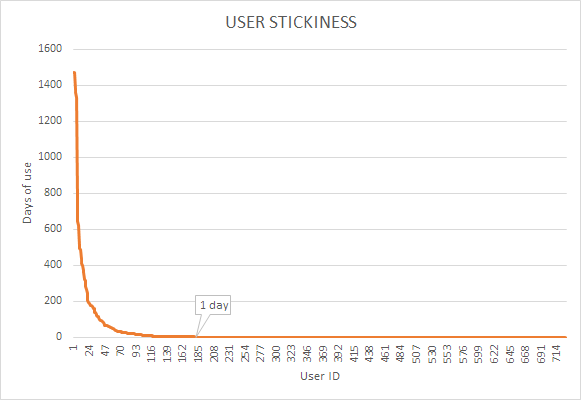
\includegraphics[width=1\textwidth]{figures/userStickiness.png}
	\caption{Distribution of usage duration for users}
	\label{fig:userstickiness}
\end{figure}

While this distribution is not too impressive for the commercial product, 
it is somehow expected for a research prototype without any updates and 
improvements for more than a year after it was built. It shows that the 
approach has potential and triggered interest in a decent number of the users, 
which indicates it could gain a lot of interest with a few improvements and 
obvious bug fixes.

%subsection
\subsection{Results Summary}
\label{section:resultssummary}
As a wrap-up of the result sections, \autoref{tab:baselines} shows the 
knowledge or quality contributions of particular system features and their 
appropriate baselines.

\begin{table}[h]
\centering
\caption{Contributions of separate system features and appropriate baselines}
\label{tab:baselines}
\begin{tabular}{|l|l|c|c|}
	\hline
	\makecell[c]{\textbf{System Feature}} & \makecell[c]{\textbf{Measure}} & \makecell[c]{\textbf{Baseline}} & \makecell[c]{\textbf{Proposed Approach}} \\
    \hline
	\multicolumn{4}{|c|}{\textbf{Knowledge Gathering}} \\    
    \hline
    Context and Proactivity & \makecell[l]{Number of gathered\\assertions/day} & 71 & \textbf{42.1} \\
     \hline
     \multirow{2}{10em}{Follow-up assertions (new knowledge due to already collected k.} & \makecell[l]{Number of gathered\\assertions} & 35,140 & \textbf{57,978} \\
	\cline{2-4}
																						       & \makecell[l]{Number of gathered \\assertions per concept} & 0 & \textbf{4.22} \\
	\hline 
	\multirow{2}{10em}{Cross-user assertions} & \makecell[l]{Number of gathered\\assertions\\(extrapolated)} & 43,920 & \textbf{57,978} \\
	\cline{2-4}
										     & \makecell[l]{Number of gathered\\assertions/concept} & 0 & \textbf{2.73} \\
	\hline
	\multicolumn{4}{|c|}{\textbf{Quality Control}} \\    
	\hline
	Consistency Checking & \makecell[l]{Number of removed\\bad answers} & 0 & \textbf{1420} \\
	\hline
	Crowd Voting & \makecell[l]{Number of removed\\bad answers} & 0 & \textbf{733}\\
	\hline
\end{tabular}
\end{table}

As the overall sanity check of the KB, we randomly picked 100 newly acquired 
assertions, and assessed them manually to see whether they were:
\begin{itemize}
\item Valid (in the sense of consistent with the KB here we expect 100\%)
\item True (in the sense of true in an interpretation based on our human world)
\item Useful (useful for a potential user, or for the inference engine in 
producing suggestions, validations, new questions)
\end{itemize}

The counts are presented in \autoref{tab:validity}. As expected all the 
assertions are 
valid, 96\% of them are true and 95\% are useful. This can be used as an 
estimate of the knowledge that we acquired through the proposed approach.

%old table XII
\begin{table}[h]
\centering
\caption{Results of manual evaluation on 100 randomly picked assertions}
\label{tab:validity}
\begin{tabular}{|c|c|c|}
	\hline
	\textbf{Valid} & \textbf{True} & \textbf{Useful} \\
    \hline
	100 & 96 & 95 \\    
    \hline
\end{tabular}
\end{table}

The results of this counting are not surprising, since the system doesnt allow 
manifestly inconsistent assertions, and the crowdsourcing mechanism already 
weeded out most of the untrue examples. There were four untrue assertions in 
the sample, which expose three potential problems:
\begin{enumerate}
\item One error was because the price of the coffee changed since the last 
check with the users  the stored knowledge was obsolete.
\item There were two concepts with exactly the same name and were both 
subclasses of $Organization$, so the users and also the system didnt manage to 
distinguish them and picked the wrong one. For users, everything seemed 
perfectly correct even though a logical error resulted.
\item Twice the user entered a complex sentence instead of a name of the 
concept and that forced the system to create a concept with that name (a
consequence of disabled SCG (see \autoref{section:cycnl}).
\end{enumerate}

Looking more in details of the usefulness of the retrieved knowledge, there 
were two answers, which related to the internal KB mechanism (how to handle 
events) and were thus not really useful for the end user. The remaining there 
were mostly too specific and not really useful in general, such as the name of 
the spider the user has in the corner of a room.


%
% If parts are used, the \chapteroutsidepart command must be called before final
 chapters that 
% regard all parts
%\chapteroutsidepart 
%
% Conclusions
%--------------------------------------------------------------------------------------------------
% 
\chapter{Conclusions}
%--------------------------------------------------------------------------------------------------

We came to the following conclusions \dots

%%%%%%%%%%%%%%%%%%%%%%%%%%%%%%%%%%%%%%%%%%%%%%%%%%%%%%%%%%%%%%%%%%%%%%%%%%%%%%%%
% Template Introduction

%%--------------------------------------------------------------------------------------------------
% 
\chapter{Introduction}
%--------------------------------------------------------------------------------------------------

\section{Thesis Structure}

The thesis should be structured as follows (note that while some parts are optional, their order is not):
\begin{itemize}
	\item \emph{Front Matter}
	\begin{itemize}
		\item Title pages
		\item Dedication (optional)
		\item Acknowledgments
		\item Abstract
		\item Povzetek
		\item Contents
		\item List of Figures (required if the thesis contains figures)
		\item List of Tables (required if the thesis contains tables)
		\item List of Algorithms (required if the thesis contains algorithms)
		\item Abbreviations (optional)
		\item Symbols (optional)
		\item Glossary (optional)
	\end{itemize}
	\item \emph{Main Matter}\footnote{The PhD thesis can also be divided into Parts --- this is not encouraged, but possible and supported by this template.}
	\begin{itemize}
		\item 1 Introduction
		\item $2, \dots, n-1$ Chapters
		\item $n$ Conclusions
	\end{itemize}
	The Introduction must clearly summarize the thesis from the topic application of the doctoral dissertation. The core text of the doctoral dissertation can be substituted by publications (or papers accepted for publication) in internationally recognized journals. In this case, the Introduction should clearly describe the scientific method and the candidate’s contribution to any publication which has been produced by several authors. In the Discussion or Conclusions, the candidate should summarize coherently the results of his/her dissertation.
	\item \emph{Appendices} (optional)
	\begin{itemize}
		\item Appendix A Title
		\item Appendix B Title
		\item \dots
	\end{itemize}
	If desired, the candidate can place some of his/her relevant papers in the appendices. In order to do so, he/she must obtain permissions from publishers.
	\item \emph{Back Matter}
	\begin{itemize}
		\item References
		\item Bibliography 
		\item Biography
		\item Index (optional)
	\end{itemize}
\end{itemize}

In addition, each author must prepare the cover page and spine using the two \texttt{.doc} files provided by IPS.

\section{Sectioning Example}

This is a section. Some more text. Some more text. Some more text. Some more text. Some more text. Some more text. Some more text. Some more text. Some more text. Some more text. Some more text. Some more text. 

Some more text. Some more text. Some more text. Some more text. Some more text. Some more text. Some more text. Some more text. Some more text. Some more text. Some more text. Some more text. 

\subsection{Subsection}

This is a subsection. Some more text. Some more text. Some more text. Some more text. Some more text. Some more text. Some more text. Some more text. Some more text. Some more text. Some more text. Some more text. 

Some more text. Some more text. Some more text. Some more text. Some more text. Some more text. Some more text. Some more text. Some more text. Some more text. Some more text. Some more text. 

\subsubsection{Subsubsection}

This is a subsubsection. Some more text. Some more text. Some more text. Some more text. Some more text. Some more text. Some more text. Some more text. Some more text. Some more text. Some more text. Some more text. 

Some more text. Some more text. Some more text. Some more text. Some more text. Some more text. Some more text. Some more text. Some more text. Some more text. Some more text. Some more text. 

\paragraph{Paragraph}

This is a paragraph. Some more text. Some more text. Some more text. Some more text. Some more text. Some more text. Some more text. Some more text. Some more text. Some more text. Some more text. Some more text.  

Some more text. Some more text. Some more text. Some more text. Some more text. Some more text. Some more text. Some more text. Some more text. Some more text. Some more text. Some more text. 

\subparagraph{Subparagraph}

This is a subparagraph. It is not possible to get deeper than this. Some more text. Some more text. Some more text. Some more text. Some more text. Some more text. Some more text. Some more text. Some more text. Some more text. Some more text. Some more text. 

Some more text. Some more text. Some more text. Some more text. Some more text. Some more text. Some more text. Some more text. Some more text. Some more text. Some more text. Some more text. 

\subparagraph{Subparagraph}

This is a subparagraph. It is not possible to get deeper than this. Some more text. Some more text. Some more text. Some more text. Some more text. Some more text. Some more text. Some more text. Some more text. Some more text. Some more text. Some more text. 

\paragraph{Paragraph}

This is a paragraph. Some more text. Some more text. Some more text. Some more text. Some more text. Some more text. Some more text. Some more text. Some more text. Some more text. Some more text. Some more text. 

\subsubsection{Subsubsection}

This is a subsubsection. Some more text. Some more text. Some more text. Some more text. Some more text. Some more text. Some more text. Some more text. Some more text. Some more text. Some more text. Some more text.  

\paragraph{Paragraph}

This is a paragraph. Some more text. Some more text. Some more text. Some more text. Some more text. Some more text. Some more text. Some more text. Some more text. Some more text. Some more text. Some more text.  

\paragraph{Paragraph}

This is a paragraph. Some more text. Some more text. Some more text. Some more text. Some more text. Some more text. Some more text. Some more text. Some more text. Some more text. Some more text. Some more text. 

\subsection{Subsection}

This is a subsection. Some more text. Some more text. Some more text. Some more text. Some more text. Some more text. Some more text. Some more text. Some more text. Some more text. Some more text. Some more text. 

\subsubsection{Subsubsection}

This is a subsubsection. Some more text. Some more text. Some more text. Some more text. Some more text. Some more text. Some more text. Some more text. Some more text. Some more text. Some more text. Some more text. 

\subsubsection{Subsubsection}

This is a subsubsection. Some more text. Some more text. Some more text. Some more text. Some more text. Some more text. Some more text. Some more text. Some more text. Some more text. Some more text. Some more text. 

%
% If needed, the thesis can consist of parts (not encouraged)
%\part{First Part of the Thesis}
%
% Second chapter 

%%--------------------------------------------------------------------------------------------------
% 
\chapter{Floating Bodies}
%--------------------------------------------------------------------------------------------------

Floating bodies are figures, tables and algorithms. 

\section{Figures}

Captions should be placed below figures as shown in \figurename~\ref{fig:ips-short}. If a caption is shorter than the line width, it should be centered. 

\begin{figure}[htb]
	\centering
		
\includegraphics[width=0.4\textwidth]{figures/ipslogo-cut.pdf}
	\caption{A large IPS logo.}
	\label{fig:ips-short}
\end{figure}

On the other hand, if a caption is very long (see \figurename~\ref{fig:ips-long}), only its first (short) part should be put in the List of Figures. 

\begin{figure}[htb]
	\centering
		
\includegraphics[width=0.15\textwidth]{figures/ipslogo-cut.pdf}
	\caption[A small IPS logo.]{A small IPS logo. The IPS has its own logo and a uniform graphic image, which is used on all its documents.}
	\label{fig:ips-long}
\end{figure}

\section{Tables}

Similar rules apply also to captions of tables, with the exception that captions are placed above tables (see \tablename~\ref{tab:example}).

\begin{table}[htb]
	\caption{A simple table.}
	\label{tab:example}
	\centering
		\begin{tabular}{ccc}
			\hline
			A & B & C \\
			\hline
			12 & 9834 & 327 \\
			51 & 2234 & 97 \\
			\hline
		\end{tabular}
\end{table}

\section{Algorithms}

Algorithm~\ref{alg:myalgorithm} presents an algorithm example. 

\begin{algorithm}[htb]
	\caption{An algorithm example.}
	\label{alg:myalgorithm}

	\vspace{5pt}
	\KwData{this text}
	\KwResult{complete understanding}
	\vspace{5pt}
	initialization\;
	\While{not at end of this document}{
		read current section\;
		\eIf{understood}{
			go to next section\;
			current section becomes this one\;
		}{
			go back to the beginning of current section\;
		}	
	}
\end{algorithm}

%
% Third chapter template

%%--------------------------------------------------------------------------------------------------
% 
\chapter{Equations and Measurement Units}
%--------------------------------------------------------------------------------------------------

\section{Equations}

Small equations are often written in-line (within the text), for example $j^\star = \sigma T^4$, while larger ones need to be displayed in the following way:
\begin{equation}
	\sigma = \frac{2 \pi^5 k^4}{15 c^2 h^3} = 5.6704 \times 10^{-8} J s^{-1} m^{-2} K^{-4}
	\label{eq:complex}
\end{equation}
All displayed equations need to be numbered so that they can be referenced later in the text (for example, Eq.~(\ref{eq:complex}) presents the Stefan's (or Stefan-Boltzmann) constant).

\section{Measurement Units}

The candidate can choose a standard for measurement units and has to consistently use it throughout the thesis. 

%
%\part{Second Part of the Thesis}
%
% Fourth chapter 

%%--------------------------------------------------------------------------------------------------
% 
\chapter{Definitions and Theorems}
%--------------------------------------------------------------------------------------------------

\section{Definitions}

See the formal definition of the right triangle in Definition~\ref{def:right-triangle}.

\begin{definition}[Right triangle]
\label{def:right-triangle}
A \emph{right triangle} is a triangle in which one angle is a 90-degree angle.
\end{definition}

\section{Theorems}
\label{sec:theorems}

The Pythagorean theorem is a relation in Euclidean geometry among the three sides of a right triangle. It states that the square of the hypotenuse (the side opposite the right angle) is equal to the sum of the squares of the other two sides \parencite{pythagoras}. \index{Pythagorean theorem!theorem}

\begin{theorem}[Pythagorean theorem]
\label{thm:pythagoras}
In every right triangle with sides $a$ and $b$ and hypotenuse $c$, the following holds:
\begin{equation}
a^2 + b^2 = c^2
\end{equation}
\end{theorem}

See Appendix~\ref{app:proofs} for the proof of this theorem.

%
% Fifth chapter 

%%--------------------------------------------------------------------------------------------------
% 
\chapter{Reference Formatting}
%--------------------------------------------------------------------------------------------------

References should be formatted using either the IEEE or APA 6th edition formatting style. This template uses the latter one. 

\section{IEEE}

Please see the template using the IEEE style. 

\section{APA 6th Edition}

References are cited using the \texttt{\textbackslash parencite} command. For example, see \parencite{mihailovic06}. The alternative \texttt{\textbackslash textcite} is used when the authors are mentioned in text. For example, let us cite the work by \textcite{depolli13}. References to journal articles that have not yet been published should contain the \texttt{doi}, as in \parencite{tusar14}.

Multiple references can be cited at the same time \parencite{kobal04,grace10,novak12eng,zupanc13}. Beside books and journal articles, parts of books \parencite{smodis09}, technical reports \parencite{ivekovic13eng}, PhD theses \parencite{dovgan14eng} and MSc theses \parencite{tusar07eng} can be included in the references.

Finally, on-line sources can be referenced, too, see Section~\ref{sec:theorems}.

%-------------------------------------------------------------------------------
%
% APPENDICES (optional)
%-------------------------------------------------------------------------------
%
%\appendix
%\begin{appendices}
%%
%% For example, proofs of theorems could be an appendix
%%-------------------------------------------------------------------------------
% 
\chapter{Proofs of Theorems}
\label{app:proofs}
%-------------------------------------------------------------------------------

\section{Proof of the Pythagorean Theorem}
\index{Pythagorean theorem!proof}

Let us prove the Pythagorean Theorem from page~\pageref{thm:pythagoras}.

\begin{proof}
This proof is based on the proportionality of the sides of two similar triangles, that is, upon the fact that the ratio of any two corresponding sides of similar triangles is the same regardless of the size of the triangles.

Let $ABC$ represent a right triangle, with the right angle located at $C$, as shown in Figure~\ref{fig:Pythagoras}. We draw the altitude from point $C$, and call $H$ its intersection with the hypotenuse $AB$. Point $H$ divides the length of the hypotenuse into two parts. 

\begin{figure}[htb]
	\centering
		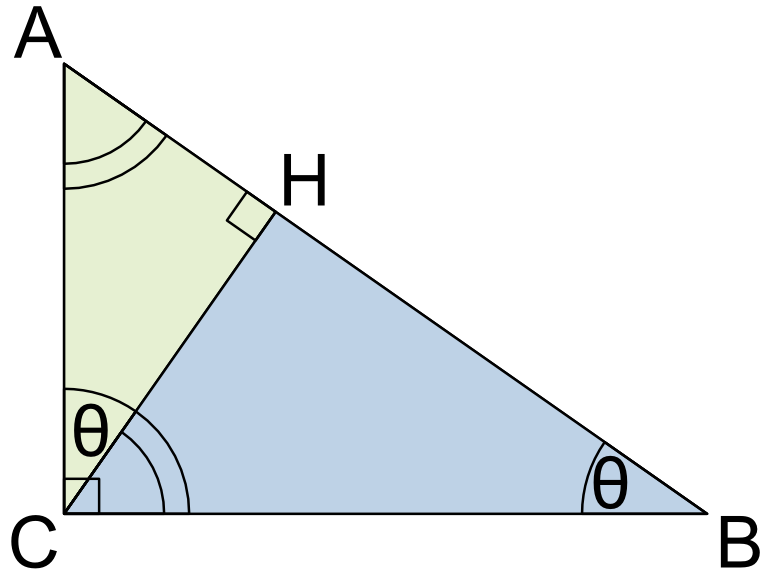
\includegraphics[width=0.3\textwidth]{figures/Pythagoras.png}
	\caption{Similar triangles used in the proof of the Pythagorean theorem.}
	\label{fig:Pythagoras}
\end{figure}

The new triangle $ACH$ is similar to triangle $ABC$, because they both have a right angle (by definition of the altitude), and they share the angle at $A$, meaning that the third angle will be the same in both triangles as well, marked as $\theta$ in Figure~\ref{fig:Pythagoras}. By a similar reasoning, the triangle $CBH$ is also similar to $ABC$. 

Similarity of the triangles leads to the equality of ratios of corresponding sides:
\begin{equation}
    \frac{BC}{AB}=\frac{BH}{BC} \text{ and } \frac{AC}{AB}=\frac{AH}{AC}.
\end{equation}
The first result equates $\cos \theta$ and the second result equates $\sin \theta$.

These ratios can be written as:
\begin{equation}
    {BC}^{2}={AB}\times {BH} \text{ and }{AC}^{2}={AB}\times {AH}.
\end{equation}
Summing these two equalities, we obtain:
\begin{equation}
    {BC}^{2}+{AC}^{2}={AB}\times {BH}+{AB}\times {AH}={AB}\times({AH}+{BH})={AB}^{2} ,
\end{equation}
which, tidying up, is the Pythagorean theorem:
\begin{equation}
    {BC}^{2}+{AC}^{2}={AB}^{2}.
\end{equation}
\end{proof}

%%
%\end{appendices}
%-------------------------------------------------------------------------------
%
% BACK MATTER
%-------------------------------------------------------------------------------
%
\backmatter
%
% References used in the thesis
\printreferences
% 
% Author's bibliography 
%-------------------------------------------------------------------------------
% 
\chapter{Bibliography}
%------------------------------------------------------------------------------
% Enclose with refsection and use \nocite{*}, if you need to list publications 
%not referenced in the thesis:
\begin{refsection}
\nocite{*}

\section*{Publications Related to the Thesis}

\defbibheading{subbibliography}{\subsection*{Journal Articles}}
\printbibliography[heading=subbibliography,keyword=myarticle]

\defbibheading{subbibliography}{\subsection*{Conference Paper}}
\printbibliography[heading=subbibliography,keyword=myconf]

\defbibheading{subbibliography}{\subsection*{Book Chapter}}
\printbibliography[heading=subbibliography,keyword=mybook]

\defbibheading{subbibliography}{\subsection*{Magazine Article}}
\printbibliography[heading=subbibliography,keyword=mymagazine]


%\section*{Other Publications (optional)}
%\dots

\end{refsection}

%
% Author's biography
%-------------------------------------------------------------------------------
% 
\chapter{Biography}
%-------------------------------------------------------------------------------

The author of this thesis is PhD candidate from Artificial Intelligence Lab at 
Jožef Stefan Institute, Slovenia. His research interests and PhD topic are in 
Natural Language Processing, Logical Inference, Knowledge Extraction and
Crowdsourcing. In 2010 he graduated from Faculty of Electrical Engineering and
started his doctoral studies at Jožef Stefan International Postgraduate School.
He worked as an Artificial Intelligence and Machine Learning researcher at
Jožef Stefan Artificial Intelligence Laboratory since 2005 on the topics related
to this thesis. From 2008 to 2013 he also worked as a principal software 
engineer for Cycorp Europe, which was at the time an EU branch of the American 
AI company Cyc Inc. During these years, he worked on an EU project developing 
distributed large scale inference engine (LarKC), and also on an AI assistant 
built on top of Cyc which lead to the development and implementation of the
approach described in this thesis. Some of the recent projects with a similar
topic include a concept of an intelligent motorhome (reasoning engine software 
interacting with sensors and actuators) for a European motorhome producer 
(Adria Mobil) and Named Entity Disambiguation algorithm which is a work in 
progress in collaboration with US Company Bloomberg L.P.

%
% Index (optional)
\printmyindex
%-------------------------------------------------------------------------------
\end{document}
